%%%%%%%%%%%%%%%%%%%%%%% file template.tex %%%%%%%%%%%%%%%%%%%%%%%%%
%
% This is a general template file for the LaTeX package SVJour3
% for Springer journals.          Springer Heidelberg 2010/09/16
%
% Copy it to a new file with a new name and use it as the basis
% for your article. Delete % signs as needed.
%
% This template includes a few options for different layouts and
% content for various journals. Please consult a previous issue of
% your journal as needed.
%
%%%%%%%%%%%%%%%%%%%%%%%%%%%%%%%%%%%%%%%%%%%%%%%%%%%%%%%%%%%%%%%%%%%
%
% First comes an example EPS file -- just ignore it and
% proceed on the \documentclass line
% your LaTeX will extract the file if required
\begin{filecontents*}{example.eps}
%!PS-Adobe-3.0 EPSF-3.0
%%BoundingBox: 19 19 221 221
%%CreationDate: Mon Sep 29 1997
%%Creator: programmed by hand (JK)
%%EndComments
gsave
newpath
  20 20 moveto
  20 220 lineto
  220 220 lineto
  220 20 lineto
closepath
2 setlinewidth
gsave
  .4 setgray fill
grestore
stroke
grestore
\end{filecontents*}
%
\RequirePackage{fix-cm}
%
%\documentclass{svjour3}                     % onecolumn (standard format)
%\documentclass[smallcondensed]{svjour3}     % onecolumn (ditto)
\documentclass[smallextended]{svjour3}       % onecolumn (second format)
%\documentclass[twocolumn]{svjour3}          % twocolumn
%
\smartqed  % flush right qed marks, e.g. at end of proof
%
\usepackage[usenames,dvipsnames]{xcolor}
\usepackage{graphicx}
\usepackage{hyperref}
\usepackage{mathrsfs,amsmath,amssymb,amscd,mathtools}
\usepackage{booktabs}
\usepackage{graphicx}
\usepackage{lscape}
\usepackage{color}
\usepackage{multirow}
\usepackage{booktabs}
\usepackage{subfig}
\usepackage{float}
\usepackage{caption}
\usepackage{filecontents}
\usepackage[normalem]{ulem}
\usepackage[flushleft]{threeparttable}
\usepackage{stfloats}
\usepackage{lscape}
\usepackage{longtable}
\usepackage{listings}
\usepackage{courier}
\usepackage{soul}


\lstdefinelanguage{julia}
{
	sensitive=true,	
           basicstyle=\ttfamily\scriptsize,
	columns=fullflexible, % make sure to use fixed-width font, CM typewriter is NOT fixed width
	numbers=left, 
	numberstyle=\small\ttfamily\color{Gray},
	stepnumber=0,              
	numbersep=10pt, 
	numberfirstline=true, 
	numberblanklines=true, 
	tabsize=4,
	lineskip=-1.5pt,
	extendedchars=true,
	breaklines=true,        
	keywordstyle=\color{Blue}\bfseries,
	identifierstyle=, % using emph or index keywords
	commentstyle=\sffamily\color{OliveGreen},
	stringstyle=\color{Maroon},
	showstringspaces=false,
	showtabs=false,
	upquote=false,
	keywordsprefix=\@,
	keywords={exit,whos,edit,load,is,isa,isequal,typeof,tuple,ntuple,uid,hash,finalizer,convert,promote,
		subtype,typemin,typemax,realmin,realmax,sizeof,eps,promote_type,method_exists,applicable,
		invoke,dlopen,dlsym,system,error,throw,assert,new,Inf,Nan,pi,im,begin,while,for,in,return,
		break,continue,macro,quote,let,if,elseif,else,try,catch,end,bitstype,ccall,do,using,module,
		import,export,importall,baremodule,immutable,local,global,const,Bool,Int,Int8,Int16,Int32,
		Int64,Uint,Uint8,Uint16,Uint32,Uint64,Float32,Float64,Complex64,Complex128,String,Symbol,Any,Nothing,None,
		function,type,typealias,abstract},
	comment=[l]{\#},
	%morecomment=[s]{#=}{=#},
	morestring=[d]\',
	morestring=[b]\",
}


\graphicspath{{./figures/}}

% set table of contents depths
\setcounter{tocdepth}{2}

% set shortcuts
%% Package, Library, abbreviate terms
\newcommand{\siplibtwo}{\textsf{SIPLIB 2.0}}
\newcommand{\siplib}{\textsf{SIPLIB}}
\newcommand{\miplib}{\textsf{MIPLIB 2010}}
\newcommand{\smps}{\textsf{SMPS}}
\newcommand{\mps}{\textsf{MPS}}
\newcommand{\mpsx}{\textsf{MPSX}}
\newcommand{\jump}{\textsf{JuMP}}
\newcommand{\structjump}{\textsf{StructJuMP}}

% Problems
\newcommand{\dcap}{\textsf{DCAP}}
\newcommand{\dclp}{\textsf{DCLP}}
\newcommand{\mptsps}{\textsf{MPTSPs}}
\newcommand{\sizes}{\textsf{SIZES}}
\newcommand{\smkp}{\textsf{SMKP}}
\newcommand{\sslp}{\textsf{SSLP}}
\newcommand{\suc}{\textsf{SUC}}

% Solvers
\newcommand{\dsp}{\textsf{DSP}}
\newcommand{\pysp}{\textsf{PySP}}
\newcommand{\pyomo}{\textsf{Pyomo}}
\newcommand{\cplex}{\textsf{CPLEX}}

%% Programming languages
\newcommand{\julia}{\texttt{Julia}}
\newcommand{\python}{\texttt{Python}}
\newcommand{\clang}{\texttt{C}}
\newcommand{\cpp}{\texttt{C++}}
\newcommand{\matlab}{\texttt{MATLAB}}

%% Siplib.jl related terms
\newcommand{\jumpmodel}{\texttt{JuMP.Model}}
\newcommand{\siplibjl}{\texttt{Siplib.jl}}

\newcommand{\kk}[1]{{\color{blue}From Kibaek: #1}}
\newcommand{\yoc}[1]{{\color{purple}From Yongkyu: #1}}
\newcommand{\stkout}[1]{\ifmmode\text{\sout{\ensuremath{#1}}}\else\sout{#1}\fi}
\DeclareMathOperator*{\PP}{\mathbb{P}}
\DeclareMathOperator*{\EE}{\mathbb{E}}
\DeclarePairedDelimiter\ceil{\lceil}{\rceil}
\DeclarePairedDelimiter\floor{\lfloor}{\rfloor}

\raggedbottom
% \usepackage{mathptmx}      % use Times fonts if available on your TeX system
%
% insert here the call for the packages your document requires
%\usepackage{latexsym}
% etc.
%
% please place your own definitions here and don't use \def but
% \newcommand{}{}
%
% Insert the name of "your journal" with
% \journalname{myjournal}
%

\begin{document}
\title{SIPLIB 2.0
%\thanks{Grants or other notes
%about the article that should go on the front page should be
%placed here. General acknowledgments should be placed at the end of the article.}
}
\subtitle{Stochastic Integer Programming Test Problem Library 2.0}

\titlerunning{SIPLIB 2.0}        

\author{Yongkyu Cho \and 
		Kibaek Kim \and
        Cong Han Lim \and
        James Luedtke \and
        Jeffrey Linderoth
}

%\authorrunning{Short form of author list} % if too long for running head

\institute{Yongkyu Cho \at
			Department of Industrial and Management Engineering, Pohang University of Science and Technology, Gyeongbuk, Korea \\
			\email{jyg1124@postech.ac.kr}
			\and
			Kibaek Kim \at
           Mathematics and Computer Science Division, Argonne National Laboratory, Lemont, IL 60439, USA \\
           \email{kimk@anl.gov}
           \and
           Cong Han Lim \and James Luedtke \and Jeffrey Linderoth \at
           Department of Industrial and Systems Engineering, University of Wisconsin-Madison Madison, WI 53706, USA \\
           \email{clim9@wisc.edu; jim.luedtke@wisc.edu; linderoth@wisc.edu}
}

\date{Received: date / Accepted: date}

\maketitle

% abstract
\begin{abstract}
The first \siplib\ was constructed in 2002 by Shabbir Ahmed and his colleagues. The library has been providing a collection of test instances to facilitate computational and algorithmic research in SIP. State-of-the-art in SIP combined with the speedup in computing machinery, however, has made many \siplib\ instances trivial.
By \siplibtwo\, we provide 1) richer collection of test instances with benchmarking computational results, 2) not only \texttt{SMPS} files but also utilities for generating/analyzing instances. \siplibtwo\ is implemented in Julia programming language with modeling package \texttt{StructJuMP} (block-structured optimization framework for Julia mathematical programming).
\keywords{SIPLIB \and Stochastic Integer Programming \and Problem Instances \and Julia programming language}
\end{abstract}
\pagebreak

% lists (tableofcontents, figures, tables)
\tableofcontents
\pagebreak

\listoftables
\pagebreak

\listoffigures
\pagebreak

\section{Introduction}\label{sec:intro}
%(What SIP is and our restriction) 
Stochastic (mixed) integer programming (SIP) is the mathematical programming that accounts for 
both continuous and discrete decision variables with uncertain parameters~\cite{book:BL2011}. 
Modeling and algorithms for SIP have been advanced for the last few decades. Applications of SIP include power systems~\cite{?}, healthcare~\cite{?}, manufacturing systems~\cite{?}, and transportation~\cite{?}. With the advances, a number of solution methods have been developed and shown to be computationally effective for stochastic problems (e.g.,~\cite{?}). Moreover, many of the algorithms have been implemented as software packages either specific for certain problems~\cite{?} or for generic problems~\cite{?}.

Numerical tests and benchmarks are necessary for developing and improving algorithms. However,
these have been challenging for the stochastic programming community, because of the limited number of test problem instances. SIPLIB is a set of test problem instances for SIP available in~\url{https://www2.isye.gatech.edu/~sahmed/siplib/}, where nine problem instances are available in SMPS format~\cite{?} with additional information such as random parameters, 
instance size, best known objective value or bounds, optimality gap, and solution time.  

In this paper, we focus on two-stage SIP with 
linear objective function and constraints, where the first stage finds a solution before the 
random parameters are realized, and the second stage takes a recourse action to the 
uncertainty realization for a given first-stage decision. We assume that the random realization of problem parameters (i.e., scenarios) are discrete and finite with known probabilities.
A key challenge in SIP is that the size of
the problem increases with the number of scenarios. The main difficulty in solving two-stage SIP is that the 
second-stage value function is not necessarily convex. Thus, the standard decomposition 
approaches that work nicely for stochastic \textit{linear} programs, break down when the 
second stage integer variables are present \cite{journal:AG2004}. Hereinafter, we use the 
term SIP to indicate the two-stage SIP. 


%\subsection{Literature review} \label{subsec:literaturereview}
Meanwhile, the optimizers, not only SIP researchers, have always needed test instances to 
figure out the performances of newly developed methods. \miplib\ \cite{MIPLIB} for mixed 
integer (linear) programming (MIP) is a good example of such collection, which comprises 361 
instances. The authors collected the instances from various sources and categorized them into 
several groups after the computational experiments. \miplib\ provides instances in 
\textsf{MPS} format with a test engine developed to run different solvers in a defined way to 
check the answers for consistency. 

%(website: Derek Holmes, POSTS, 1993)
For SP, to the best of our knowledge, the first such approach is Holmes and Birge's 
\textit{portable stochastic programming test set} (POSTS) \cite{POSTS} since 1994. POSTS is 
still available and provides a small test set of stochastic programming recourse problems in 
\smps\ format. POSTS consists of 15 problems but not dedicated to SIP. Birge 
\cite{POSTSresults} provides some computational results of the POSTS instances, but most of 
them needs to be updated. Moreover, accompanied information on the instances does not seem to 
be enough. 

%(website and paper: Andy Felt, Jason Sarich, and K. A. Ariyawansa, Test-Problem Collection 
%for Stochastic Linear Programming, 2001-2004)
Ariyawansa and Felt \cite{journal:AF2004} have constructed a test problem collection for SP 
since 2001. Unlike Holmes and Birge's work, the authors provide an accompanied document 
explaining short description, mathematical problem statement, and notational reconciliation 
to a standard problem format for each of the 9 problems. Ariyawansa and Felt's collection 
includes 3 problems that contain mixed integer variables. However, still the library is not 
dedicated to SIP and size of the instances are not large enough to perform intensive 
computational experiments. 

%(website: SIPLIB 1)
The first SIP-oriented instance collection is the \siplib\ \cite{web:SIPLIB1} constructed in 
2002 by Shabbir Ahmed and his colleagues. The instances are basically given in \smps\ format 
accompanied with simple information on the problem and computational experiment. Although 
\siplib\ provides basic ingredient to be exploited for SIP research, it has rooms for 
improvement. First, \siplib\ only provides static instances and sometimes does not even 
provide ready-to-use instance files, which limits usability of the library. Moreover, the 
precise information for implementing the original problem is sometimes not allowed. Second, 
we need more problems of various types. Considering three types of variables (continuous, 
binary, integer) and two stages, the possible number of combination is $\left[\sum_{k=1}
^3\binom{3}{k}\right]^2=49$ in total while \siplib\ provides only 5 such combinations 
regarding the problems that can be fully implementable based on the open information.
Third, \siplib\ needs to be polished systematically in terms of both pre-analysis on the 
instances and post-analysis on the benchmark results. Currently, there is no predefined 
contribution rule for \siplib\ so different problem provides different information. 
Therefore, interpretation on the new results can be inconsistent.

%(Motivation) 
%At the time \siplib\ appeared, it provided enoughly large-sized instances that is reasonable 
to argue that the performance of algorithm is remarkable if it handles the instances well. 
State-of-the-art in SIP combined with the speedup in computing machinery, however, makes many 
instances in \siplib\ trivial so that we have not enough basis to use them for showing the 
excellence of newly suggested solution methods. At this point, we are motivated to develop 
the second version of \siplib\, say \siplibtwo\ that provides larger-sized test instances 
with higher degree of tailorability, e.g., users can easily generate instances of test 
problems as largely as they want.% in terms of the number of scenarios included.

%At the time \siplib\ appeared, it provided enough instances to be used for computational 
experiments of SIP methods. State-of-the-art in SIP combined with the speedup in computing 
machinery, however, requires more test sets as the existing instances have been conquered 
gradually. As \siplib\ only provides limited testing resources (e.g., static instance files), 
it has less expandability. 
Based upon the current limitations of \siplib, we conclude that the current \siplib\ needs to 
be improved since state-of-the-art in SIP combined with the speedup in computing machinery 
requires more test sets. At this point, we are motivated to develop the second version of 
\siplib, say \siplibtwo, that includes richer testing resources. By ``richer", we mean the 
three things. First, instances of the different type of problems other than existing ones. 
Second, the larger-sized instances of the existing \siplib\ problems. Third, higher degree of 
freedom for the researchers, e.g., users can easily generate instances of the size/shape as 
they want.

%(SMPS, Julia)
We provide \siplibtwo\ in two ways: \smps\ files (*.cor, *.tim, *.sto) and open-source 
\julia\ package. \smps\ is a file format widely used to describe stochastic program 
instances. Once \smps\ files are given, we can directly solve it using SIP solvers like \dsp\ 
\cite{journal:KZ2015} and \textsf{SMI} \cite{web:SMI}. A drawback of \smps\ is low 
readability by human, which we decided to provide \julia\ scripts to let users be able to 
easily catch up the problems and tailor the instances if needed.

%(Convenience of Julia) 
\julia\ is an open-source high-level, high-performance dynamic programming language for 
numerical computing. It is also known as good performance, approaching that of statically-
compiled languages like \clang\ \cite{journal:BEKS2017}. The syntax of \julia\ is simple and 
should feel familiar to anyone who has experienced in another high-level languages like 
\matlab\ or \python. A \julia\ package called \jump\ (\julia\ for Mathematical Programming 
\cite{journal:JuMP}) provides a domain-specific modeling language for mathematical 
optimization embedded in \julia. \jump\ enables us to easily translate a paper-written 
mathematical models to a \texttt{JuMP.Model}-type object. Some structured mathematical models 
like SIP can also be translated to the \texttt{JuMP.Model}-type object by loading a 
structured modeling package \structjump\ \cite{web:StructJuMP}. Once we have a \julia\ script 
for constructing \texttt{JuMP.Model}-type object, it is easy to modify the original model. 
%For each problem in \siplibtwo, we provide a \julia\ script for constructing 
\texttt{JuMP.Model}-type object. 

Using SP-related packages, we implement a new \julia\ package to provide various 
functionalities for handling \siplibtwo\ instances for users' convenience. Those who feel the 
given instances are not enough can simply generate new instances using the package.


%(Contribution of SIPLIP2.0) 
The contributions of this work can be summarized as follows.
\begin{itemize}
	\item We provide SIP-dedicated testing resources that are richer than the former \siplib.
	\item We collect, implement, summarize, and open all the problem-specific details: 
	mathematical formulation, stochastic data generation, \julia\ scripts.
	\item We implement and release an open-source \julia\ package for SIP research: 
	generating and analyzing the instances.
	\item We provide both analytical and computational information on the accompanied 
	instances.
\end{itemize}

%By \texttt{SIPLIB 2.0}, we provide 1) richer collection of test instances for computational 
and algorithmic research in SIP with benchmarking computational results, 2) not only 
\texttt{SMPS} files but also utilities for generating/analyzing instances. Hence, the users 
can obtain as large-sized instances as they need by generating new scenarios and including 
them into instances. For those who want to utilize the instances in the legacy 
\texttt{SIPLIB} with strong tailorability provided by \texttt{SIPLIB 2.0}, we include the 
original \texttt{SIPLIB} instances as well.

%(Contents)
This paper is organized as follows. In Section \ref{sec:sip}, we briefly review SIP. This 
includes the mathematical formulation with notation, solution methods, and available software 
packages. In Section \ref{sec:summary}, we provide summary and discussion of the test 
problems. This consists of origin of the problems with brief description, instance naming 
rule, problem type, the number of components, and sparsity information. We also discuss why 
they are important in each subsection. Together with the problem-specific description given 
in Section\ref{sec:prob_desc}, we believe that users can quickly catch up what they need 
without investigating every detail. In Section \ref{sec:package}, we introduce our 
implementation of a \julia\ package for \siplibtwo\ with a tutorial in Section 
\ref{sec:tutorial}. In Section \ref{sec:instance_catalog}, we report analytical and 
computational results of the accompanied \smps\ instances. We conclude this study with the 
emphasis on our spirit for further improvement in SIP in Section \ref{sec:conclusion}. 








\pagebreak

\section{Stochastic integer programming}\label{sec:sip}
In this section, we explain the general description of SIP of interest. This includes formal mathematical formulation, existing general solution methods to solve the SIPs, and currently available software libraries.
\subsection{Formulation}
%We introduce the form of SIP of interest. The notations and dimensional information are summarized in Table \ref{notation:SIP}. 

We are interested in finding the optimal solution for the two-stage SIP which is called the \textit{recourse problem} (RP): 
\begin{align}
\textrm{(RP) }\min_{x\in X} z(x):={\left\{c^\top x + \mathcal{Q}(x):\ Ax\ge b\right\}}, \label{eq:SIP_1}
\end{align}
where $\mathcal{Q}(x):=\EE_{\pmb{\xi}}\left[ \phi\left( h(\pmb{\xi})-T(\pmb{\xi})x \right) \right]$ is the expected recourse function associated with the random element $\pmb{\xi}$ defined on a probability triple $(\Xi, \mathcal{F},\PP)$.

We assume that $\pmb{\xi}$ follows a known probability distribution with the finite countable outcomes $\xi_1,\ldots,\xi_r$, called \textit{scenarios},  and respective probability of occurence $\PP(1),\ldots,\PP(r)$, i.e., $\PP(s):=\PP[\pmb{\xi}=\xi_s]$ for each $s\in\mathcal{S}:=\{1,\ldots,r\}$. When the distribution is known to be continuous, we assume that we can reasonably approximate it by a suitably discretized distribution. 

The real-valued map $\phi:\mathbb{R}^{m_2}\to\mathbb{R}$ is the optimal value of the second-stage recourse problem that is defined by
\begin{align}
\phi(t;{\xi_s}):=\min_{y_s\in Y}\left\{ q(\xi_s)^\top y_s:\ W(\xi_s)y_s \ge t \right\},\ \forall t\in\mathbb{R}^{m_2},
\end{align}
where $\xi_s$ is given by an arbitrarily realized scenario.
The sets $X\subseteq \mathbb{R}^{n_1}$ and $Y\subseteq\mathbb{R}^{n_2}$ represent restrictions on a subset of the decision variables $x$ and $y_s$, respectively. 
The first-stage data comprises $A$, $b$, and $c$. The second-stage data is given by the scenario-dependent values $T(\xi_s)$, $W(\xi_s)$, $h(\xi_s)$, and $q(\xi_s)$ (for dimensional information refer to Table \ref{notation:SIP}). Hereinafter, we use the simplified notation $(T_s,W_s,h_s,q_s)$ for the second-stage data. 

The RP (\ref{eq:SIP_1}) can be then rewritten in the \textit{extensive form} (EF)
\begin{subequations}\label{sip:ef}
\begin{align}
\textrm{(RP-EF) }\min_{x,\mathrm{y}}\ z(x,\mathrm{y}):=&\ c^{\top}x + \sum_{s=1}^{r}\PP(s) (q_s^{\top}y_s), \label{ef:obj}\\ 
\mathrm{s.t.}\ &Ax\ge b,  \label{ef:b}\\
	&T_s x+W_s y_s\ge h_s,\quad\forall s\in\{1,\ldots,r\}, \label{ef:c} \\
	&x\in X, \label{ef:d} \\
	&y_s \in Y,\quad\forall s\in\{1,\ldots,r\}, \label{ef:e}
\end{align}
\end{subequations}
where $\mathrm{y}:=\{y_1,\ldots,y_r\}$. The RP-EF explicitly describes all the random parameters so that its size increases as the number of scenarios in consideration increases.
\begin{table}[]
	\resizebox{\textwidth}{!}
	{
		\begin{threeparttable}
			\caption{Summary of notations in SIP formulation}
			\label{notation:SIP}
			\begin{tabular}{ll}
				\toprule
				\multicolumn{2}{l}{\textbf{Sets:}} \\ 
				$X\subseteq\mathbb{R}^{n_1}$	& first-stage polyhedral set (continuous, integer, binary)\\
				$Y\subseteq\mathbb{R}^{n_2}$	& second-stage polyhedral set (continuous, integer, binary)\\ 
				$\mathcal{S}=\{1,\ldots,r\}$	& index set of realizable scenarios \\ \midrule
				%$G_j$	& scenario feasibility set\\ \midrule
				\multicolumn{2}{l}{\textbf{Scalas:}} \\ 
	%			$z\in\mathbb{R}$ & optimal objective value of the SIP \\ 
				$r\in\mathbb{N}$	& total number of scenarios	\\	
				$s\in\mathcal{S}$	& index denoting scenario	\\
				$\PP(s)\in[0,1]$ & probability that scenario $s$ occurs, i.e., $\PP(s):=\PP[\pmb{\xi}=\xi_s]$ \\ \midrule
				\multicolumn{2}{l}{\textbf{Vectors:}} \\  
				$x\in\mathbb{R}^{n_1}$	& first-stage decision vector	\\
				$c\in \mathbb{R}^{n_1}$	& first-stage cost vector\\
				$b\in\mathbb{R}^{m_1}$	& first-stage RHS vector\\
				$y_s\in\mathbb{R}^{n_2}$	& second-stage decision vector under scenario $\xi_s$	\\
				$q_s:= q(\xi_s)\in\mathbb{R}^{n_2}$	& second-stage cost vector \\
				$h_s:= h(\xi_s)\in\mathbb{R}^{m_2}$	& second-stage RHS vector\\ \midrule
				%$\mathbf{0}\in\mathbb{R}^{rn_1}$	& vector filled with zeros \\ \midrule
				\multicolumn{2}{l}{\textbf{Matrices:}} \\  
				$A\in\mathbb{R}^{m_1\times n_1}$	& first-stage constraint matrix corresponds to decision vector $x$\\
				$W_s:= W(\xi_s)\in\mathbb{R}^{m_2\times n_2}$	& second-stage constraint matrix corresponds to decision vector $y_s$\\
				$T_s:= T(\xi_s)\in\mathbb{R}^{m_2\times n_1}$	& second-stage constraint matrix corresponds to decision vector $x$\\ \midrule
				%$H_j:= H(\xi_j)\in\mathbb{R}^{rm_1\times n_1}$	&	nonanticipativity constraints matrix \\ \midrule
				\multicolumn{2}{l}{\textbf{Functions:}} \\
				$\phi:\mathbb{R}^{m_2}\to\mathbb{R}$	&  optimal objective function of the second-stage program given a scenario\\
				$\mathcal{Q}:\mathbb{R}^{n_1}\to\mathbb{R}$	& recourse function (the expectation of $\phi\left( h(\pmb{\xi})-T(\pmb{\xi})x \right)$ over $\pmb{\xi}$) 	\\
				\bottomrule
			\end{tabular}
			\begin{tablenotes}
			\small
			\item $\pmb{\xi}$ is the random element that realizes by one of the possible scenarios $\xi_1,\ldots,\xi_r$.		
			\end{tablenotes}
		\end{threeparttable}
	}
\end{table} 


\subsection{Solution methods}
Assuming finite and discrete distribution, we can always formulate SIP in the EF as in Equations (\ref{ef:obj})-(\ref{ef:e}).  %much of the solution methods in SIP is studied to resolve the difficulty of optimizing the form in Equation \ref{eq:SIP_1}, 
%Much of the solution methods in SIP is studied to resolve the difficulty of optimizing the extensive form. %That is, the sum of the first-stage costs and the expected costs in the second-stage. 
Most computational solution methods in SIP assume that a single scenario evaluation is somehow tractable in a reasonable time. In reality, we often need to consider a vast number of scenario realizations. In this case, EF easily becomes a large MIP, but with a special structure in it. Solving this problem without exploiting the structure can quickly go with inefficiency. In this section, we introduce representative approaches to resolve the computational difficulties in SIP when many scenarios should be considered.

\subsubsection{Stage-wise decomposition}
In this type of algorithms, the primary purpose is to naturally optimize the objective function in Equation (\ref{eq:SIP_1}) over the set of feasible solutions for the first-stage. Briefly, the problem is decomposed stage-wisely to derive associated master and subproblem. Then, the algorithm alternately solves each problem to seek the true optimality of the original problem.
 
To be more specific, at each iteration of the algorithm, it builds an outer linearization of the second-stage recourse function and uses a solution of the first-stage problem plus this linearization \cite{book:BL2011}. This cutting plane technique is called \textit{Benders decomposition} \cite{journal:B1962} in general or the \textit{L-shaped method} in stochastic optimization, from which a variants of stage-wise decomposition methods have been derived. 

L-shaped method has long history since 1962 even before its successful application to the stochastic optimization. For SIP, however, the method required to be revised mostly due to the various kind of integrality presents in the problem. For example, the integer L-shaped method \cite{journal:LL1993} developed a cut generation method that approximates the second-stage recourse function only when the SIP is of pure binary first-stage and mixed integer second-stage. When the first-stage variables are not necessarily binary, Car{\o}e and Tind \cite{journal:CT1998} suggested a method to use the duality of the second-stage integer program to generate cuts that build the approximation of the recourse function.

\subsubsection{Scenario-wise decomposition}
The advantage of using this type algorithms is their ability to allow us naturally parallelized computation hence fully utilize state-of-the-art powerful computing cluster. Assuming the tractability of a single-scenario problem, this type algorithms are known to be one of the most effective solution methods to solve the real world large-scale problems.

To briefly explain the idea of scenario-wise decomposition, we first introduce the following terms for solution systems:
\begin{itemize}
	\item \textit{admissible}: a solution system that satisfies constraints for all scenarios
	\item \textit{implementable} (or \textit{nonanticipative}): a solution system where every scenario-specific solution has the same first-stage decision
	\item \textit{feasible}: a solution system that is both admissible and implementable
\end{itemize}

Scenario-wise decomposition starts with introducing the copies of the first-stage variables into the second-stage. Then, the RP-EF in (\ref{sip:ef}) is written as below.
\begin{subequations} \label{sip:ef'}
	\begin{align}
	\textrm{(RP-EF') }\min_{\mathrm{x},\mathrm{y}}\ z(x,y):=\ &\sum_{s=1}^{r}\PP(s)\left(c^{\top}x_s+q_s^{\top}y_s\right)	\label{eq:SIP_2-1}\\ 
	\mathrm{s.t.}\ &\sum_{s=1}^{r}H_s x_s=0, \label{eq:SIP_2-2} \\
	\ &(x_s,y_s)\in G_s,\quad \forall s\in\{1,\ldots,r\},	\label{eq:SIP_2-3}
	\end{align}
\end{subequations}
where $\mathrm{x}:=\{x_1,\ldots,x_r\}$ and the scenario feasibility set $G_s$ is defined as
\begin{align} 
G_s:=\left\{ (x_s,y_s): \ Ax_s\ge b,\  T_s x_s+W_s y_s\ge h_s,\ (x_s,y_s)\in X\times Y  \right\}. \label{eq:SIP_2-4}
\end{align}
The newly included constraints (\ref{eq:SIP_2-2}) (called \textit{nonanticipativity} constraints) guarantee $x_1=x_r$ and $x_s=x_{s-1}$ for $s=2,\ldots,r$. Here, the matrix $H_s$ is of dimension $l\times n_1$ with a suitable value $l$. %We assume that some first-stage solutions satisfying the first-stage constraints can give rise to infeasibility of RP-EF'. Without this property, the problem is called to have a (relatively) \textit{complete recourse}. 
Based on the RP-EF', there are two representative scenario-wise decomposition algorithms: Dual Decomposition (DD) and Progressive Hedging (PH). 

%We assume that SIP does not necessarily have relatively complete recourse. We recall that without this property there can exist an $\hat{x}\in X$ satisfying $A\hat{x}\ge b$ for which there does not exist a recourse $y\in\mathbb{R}^{m_2}$ satisfying $(\hat{x},y)\in G_s$ for some $s$. In other words, not every choice of the first-stage variables is guaranteed to have feasible recourse for all scenarios.

The main idea of DD algorithm is to relax the nonanticipativity constraints using Lagrange multipliers and then to restore them. Given set of multipliers, the problem is separable by scenarios hence the associated dual function can be optimized scenario-wise independently \cite{journal:CS1999}. The conceptual steps of the DD procedure can be explained as follows:
\begin{enumerate}
	\item Using Lagrangian multiplier (or dual variable) $\lambda$, relax the nonanticipativity constraints (\ref{eq:SIP_2-2}) by introducing them into the objective function (\ref{eq:SIP_2-1}).
	\item Let $k=0$ be the iteration step and set initial value on the $k$-step dual variable $\lambda^{(k)}$.
	\item Scenario-wisely decompose the relaxed problem with fixed $\lambda^{(k)}$ and solve it independently to get the $k$-step solutions.
	\item Update the best upper bound based on the $k$-step solutions.
	\item Go to step 3. with $k=k+1$ and then updating $\lambda^{(k+1)}$ based on the $k$-step solutions if the convergence criterion is yet to be satisfied.
\end{enumerate}
Due to the nonconvexities, there may exist a duality gap between relaxed problem and the original problem so that the primal feasibility needs to be attained by branch-and-bound or heuristic schemes. However, achieving that primal feasibility is not always available when the problem does not have relatively complete recourse hence a crucial limitation of DD. Nevertheless, DD is known to be one of the effective methods since it often provides an useful tight lower bounds for the original problem.

PH algorithm is developed by Rockafellar and Wets \cite{journal:RW1991} motivated by augmented Lagrangian theory. 
A brief steps of the PH procedure can be summarized as follows \cite{book:pyomo}:
\begin{enumerate}
	\item Let $k=0$ be the iteration step and $w_s^{(k)}=0$ for all $s\in\mathcal{S}$.
	\item For each scenario $s\in\mathcal{S}$, solve the problem (\ref{eq:SIP_2-1}), (\ref{eq:SIP_2-3}), and (\ref{eq:SIP_2-4}) only considering the single scenario to obtain the scenario solutions $(x_s^{(k)},y_s^{(k)})$.
	\item Then, take average of the scenario solutions to obtain an implementable first-stage decision $\bar{x}^{(k)}$.
	\item For each scenario $s$, obtain the scenario solution $(x_s^{(k+1)},y_s^{(k+1)})$ by solving the following minimization problem:
	\begin{align*}
	\min_{x_s,y_s}\left\{c^\top x_s+q_s^\top y_s + {w_s^{(k)}}^\top x_s +\frac{\rho}{2}\norm{x_s-\bar{x}^{(k)}}^2 : (x_s,y_s)\in G_s \right\},
	\end{align*}
	where ${w_s^{(k)}}:={w_s^{(k-1)}}+\rho(x_s^{(k)}-\bar{x}^{(k)})$ is the weight and $\rho$ is an algorithmic parameter for subgradient estimator, which both of them are for penalizing the lack of nonanticipativity.
%	\item For each scenario $s$, solutions are obtained for the problem of minimizing, subject to the problem constraints, the deterministic solution as in Step 1. plus terms that penalize the lack of implementability using a subgradient estimator for the nonanticipativity constraints and a squared penalty term.
	\item Go to step 2. with $k=k+1$ if the convergence criterion is yet to be satisfied. 
\end{enumerate}
A notable limitation of PH algorithm is that it does not always guarantee the convergence. However, PH is advantageous in the sense that it often provides high quality solution within a reasonable number of iterations. 
\subsection{Software libraries}
SIP considering finite number of scenarios can be represented by any algebraic modeling languages and then solved by standard MIP solvers like \cplex. However, such manual implementation without exploiting structural characteristics in SIP can easily result in inefficient computation and unnecessary memory allocation. In this subsection, we introduce some software libraries that handle SIP instances.

\subsubsection{Modeling language}
We introduce two relatively new algebraic SIP modeling languages which are compatible with general purpose high-level programming languages \julia\ and \python, respectively. Both modeling libraries are designed to allow non-specialists to easily write mathematical model on the computing environment.

\structjump\ is a \julia\ package provides a parallel algebraic modeling framework for block-structured optimization models \cite{web:StructJuMP}. \structjump\ is an extension of \jump\ modeling package (\julia\ for Mathematical Optimization \cite{journal:JuMP}), which is faster than any other modeling tools. \structjump\ enables \jump\ to express the structure of problems and efficiently interface with structure-exploiting solvers. It also works in parallel using distributed memory, and thus allows the specification of much larger problems than \jump\ can handle. Most noticeable benefit of using \structjump\ is its straightforward modeling syntax that almost feels like moving the paper-written model directly into the computer.

\pysp\ is a stochastic programming extension of a \python-based algebraic modeling package \pyomo\ \cite{book:pyomo} that supports variants of mathematical optimization. In \pysp, users can express stochastic programming problems by extending deterministic models, which are usually constructed first. To be specific, users should specify the deterministic base model with associated scenario tree presenting uncertain parameters. One advantage of using \pysp\ is its modeler-solver integration that enables users to easily get the optimization result.

\subsubsection{Solver}
Several commercial or noncommercial solvers are available for SIP. In this subsection, we mainly introduce some noncommercial solvers: \pipssbb, \scip, \dsp, and \pysp.

\pipssbb\ \cite{web:PIPS-SBB} is a distributed-memory parallel SIP solver that implements parallelized branch-and-bound (B\&B) algorithm and reads \smps\ format. The embedded scheme is designed mainly to overcome the possible memory insufficiency resulted from the B\&B procedure for a large number of scenarios. However, the computational performance in terms of speed is known to have a long way to go before it is competitive with commercial MIP solvers \cite{proceeding:MOR2016}.

\scip\ \cite{SCIP} is one of the fast non-commercial MIP and MINLP solvers that provides various optimization framework such as branching, cutting plane separation, propagation, pricing, and Benders decomposition. The latest version of \scip\ has been extended towards reading \smps\ format hence now available as an SIP solver. \scip\ currently provides two ways to solve SIP instances.
\begin{itemize}
	\item Invoking MIP solver to solve EF
	\item L-shaped method
\end{itemize}
Although \scip\ recently started to support SIP, it is still preliminary phase as an SIP-oriented solver. For example, \scip\ is yet to provide any scenario-wise decomposition algorithm that fully utilizes the special structure presents in SIP.

\dsp\ \cite{web:DSP} is an open-source SIP solver implemented in \cpp. \dsp\ also reads \smps\ files as an input format and provides three ways to solve SIP instances.
\begin{itemize}
	\item Invoking standard MIP solver to solve EF
	\item L-shaped method
	\item Dual Decomposition algorithm
\end{itemize}
\dsp\ is known as a remarkable DD-based solver and consistently improves its computational performance \cite{journal:KZ2015}. \dsp\ provides parallel implementations for the two decomposition-based algorithms, which allows users fully exploit computing clusters and multi-core processors. \dsp\ basically reads \smps\ files as input sources. In addition, \dsp\ provides \julia\ interface to improve its usability.

\pysp\ package, which we have introduced in the previous subsection, includes not only modeling framework but solver capability providing three ways to solve the instance. 
\begin{itemize}
	\item Invoking standard MIP solver to solve EF
	\item L-shaped method
	\item Progressive Hedging algorithm
\end{itemize}
\pysp's PH implementation gives an effective heuristic for approximating general multi-stage SIP \cite{journal:WWH2012}. \pysp\ also supports the distributed execution of the optimization which leverages the distributed solver capabilities that are provided in \pyomo\ library.


\pagebreak
 
\section{The test problems}\label{sec:summary}
In this section, we explain information about the test problems and corresponding instances in summarized manner. This includes problem type, components (variables and constraints), and instances for each problem. Detailed problem-specific information is available in Section \ref{sec:prob_desc} for those who are interested in.

\subsection{Type of the problems}
Table \ref{table:problems} summarizes the description of each test problem in \siplibtwo. The five of them are adopted from \siplib\ \cite{web:SIPLIB1}. We tried to implement the \siplib\ instances as same as the original references possible. Not all of them, however, are exactly the same due to insufficient information on problem parameters, e.g., random numbers in scenarios. We developed our own way to implement the problems as long as it does not harm the problem's own characteristic. 
\begin{table}[H]
	\centering
	\resizebox{\textwidth}{!}{%
		\begin{threeparttable}
		\caption{Problems in \texttt{SIPLIB 2.0}}
		\label{table:problems}
			\begin{tabular}{@{}llll@{}}
				\toprule
				Problem		  		  & Description                                                        & Main reference              \\ \midrule
				\texttt{DCAP}         & Dynamic capacity planning with stochastic demand (\ref{DCAP})                   & Ahmed and Garcia \cite{journal:AG2004}                          \\
				\texttt{DCLP}		  &	Data center location problem									   & Kim et al. \cite{journal:KYZC2017}								\\	
				\texttt{MPTSPs}       & Multi-path traveling salesman problem with stochastic travel costs (\ref{MPTSPs})& Tadei et al. \cite{journal:TPP2017}                            \\
				\texttt{SIZES}        & Optimal product substitution with stochastic demand (\ref{SIZES})         & Jorjani et al. \cite{journal:JSW1999}          \\
				\texttt{SMKP}		  & Stochastic multiple knapsack problem (\ref{SMKP})                              & Angulo et al. \cite{journal:AAD2014}                            \\
				\texttt{SSLP}         & Stochastic server location problem (\ref{SSLP})                                & Ntaimo and Sen \cite{journal:NS2005}                           \\
				\texttt{SUC}         & Stochastic unit commitment problem	(\ref{SUC})			               & Papavasiliou and Oren \cite{journal:PO2013}                       \\ \bottomrule
			\end{tabular}%
			
%			\begin{tablenotes}
%				\small
%				\item For convenience, we skip the cardinality sign $|\cdot|$ for sets, i.e., for any set $S$, $S$ denotes the number of elements $|S|$ in this table.
%			\end{tablenotes}
		\end{threeparttable}
	}
\end{table}

Table \ref{table:naming_rule} shows how we name the instances. The capital Roman letters mean the sets defining the problems and the calligraphic letter $\mathcal{S}$ means the scenario set. For notational convenience, we sometimes skip the cardinality sign $|\cdot|$ for sets, i.e., for set $S$, $S$ itself denotes the number of elements $|S|$ in Table \ref{table:naming_rule} and \ref{table:num_components}. Note that not all sets are used to define an instance. The sets that do not appear in the instance name are fixed by some pre-determined value by the original references so we follow them. For example, in \texttt{SMKP} there are 4 sets in total, $I,J,K,\mathcal{S}$, but the numbers of knapsacks $|J|$ and $|K|$ are fixed by 50 and 5.
%\begin{table}[H]
%	\centering
%	\caption{Instance naming rules}
%	\label{table:naming_rule}
%	\resizebox{\textwidth}{!}{%
%		\begin{tabular}{@{}lll@{}}
%			\toprule
%			Problem & Instance name                 & Remark                                                                    					      \\ \midrule
%			\dcap\    & DCAP\_$R$\_$N$\_$T$\_$\mathcal{S}$    &   $R$: number of resources, $N$: number of tasks, $T$: number of time periods, $\mathcal{S}$: number of scenarios        \\
%			\dclp\	 &								&																										\\
%			\mptsps\  & MPTSPs\_$D$\_$N$\_$\mathcal{S}$ &$D$: node distribution strategy, $N$: number of nodes, $\mathcal{S}$: number of scenarios\\
%			\sizes\   & SIZES\_$\mathcal{S}$                            & $\mathcal{S}$: number of scenarios   															\\
%			\smkp\    &   SMKP\_$I$\_$\mathcal{S}$    &   $I$:number of types for item, $\mathcal{S}$: number of scenarios  													 \\
%			\sslp\    &  SSLP\_$I$\_$J$\_$\mathcal{S}$      &    $I$: number of clients, $J$: number of server locations, $\mathcal{S}$: number of scenarios                 				   \\
%			\suc\    & 	SUC\_$D$\_$\mathcal{S}$    &  $D$: day type, $\mathcal{S}$: number of scenarios                                                 						 \\ \bottomrule
%		\end{tabular}%
%	}
%\end{table}

\begin{table}[H]
	\centering
	\caption{Instance naming rules}
	\label{table:naming_rule}
	\resizebox{\textwidth}{!}{%
		\begin{tabular}{@{}lll@{}}
			\toprule
			Problem & Instance name                 & Remark                                                                    					      \\ \midrule
			\dcap\    & DCAP\_$R$\_$N$\_$T$\_$\mathcal{S}$    &   $R$: number of resources, $N$: number of tasks, $T$: number of time periods, $\mathcal{S}$: number of scenarios        \\
			\mptsps\  & MPTSPs\_$D$\_$N$\_$\mathcal{S}$ &$D$: node distribution strategy, $N$: number of nodes, $\mathcal{S}$: number of scenarios\\
			\sizes\   & SIZES\_$\mathcal{S}$                            & $\mathcal{S}$: number of scenarios   															\\
			\smkp\    &   SMKP\_$I$\_$\mathcal{S}$    &   $I$:number of types for item, $\mathcal{S}$: number of scenarios  													 \\
			\sslp\    &  SSLP\_$I$\_$J$\_$\mathcal{S}$      &    $I$: number of clients, $J$: number of server locations, $\mathcal{S}$: number of scenarios                 				   \\
			\suc\    & 	SUC\_$D$\_$\mathcal{S}$    &  $D$: day type, $\mathcal{S}$: number of scenarios                                                 						 \\ \bottomrule
		\end{tabular}%
	}
\end{table}

In \siplibtwo\, we mainly classify each problem by its stage-wise variable types. We consider three types of variable: continuous, binary, and integer. Considering two stages, the possible number of combination is $\left[\sum_{k=1}^3\binom{3}{k}\right]^2=49$ in total. We try to include problems with non-overlapping such combination. Table \ref{table:prob_class} shows the stage-wise components (variable and constraints) of each problem. For the abbreviated notation on the constraints, we refer \texttt{MIPLIB 2010} \cite{MIPLIB}. Although the constraint type is possibly one of the important factors that define the problem characteristic, we decided not to consider it for classification and let this future work since it can cause too much varieties, which we cannot easily capture the insight from the problem type classification. 
\begin{table}[H]
	\centering
	\caption{Components of the problems}
	\label{table:prob_class}
	\begin{threeparttable}
		\begin{tabular}{@{}lllll@{}}
			\toprule
			& \multicolumn{2}{l}{1st stage}                              				  	& \multicolumn{2}{l}{2nd stage}                             			        \\ \midrule
			Problem 	     & Variable                    & Constraint                   	& Variable                    & Constraint                  				    \\ \midrule
			\texttt{DCAP} (\ref{dcap:formulation})    & $\mathbb{C}$, $\mathbb{B}$  & \texttt{VBB}                	& $\mathbb{B}$                & \texttt{PAR}, \texttt{M01} 			    		\\
			\texttt{DCLP}  	 &							   &								& 			 	  &													\\				
			\texttt{MPTSPs} (\ref{mptsps:formulation})  & $\mathbb{C}$, $\mathbb{B}$  & \texttt{PAR}, \texttt{GEN}		& $\mathbb{B}$                & \texttt{GEN}               						\\
			\texttt{SIZES} (\ref{sizes:formulation})   & $\mathbb{I}$ 			   & \texttt{VBD}, \texttt{GEN} 	& $\mathbb{B}$, $\mathbb{I}$  & \texttt{IKN}             						\\
			\texttt{SMKP} (\ref{smkp:formulation})   & $\mathbb{B}$                & \texttt{KNA}                	& $\mathbb{B}$                & \texttt{KNA}              						\\
			\texttt{SSLP} (\ref{sslp:formulation})   & $\mathbb{B}$                & \texttt{IVK}, \texttt{GEN} 	& $\mathbb{C}$, $\mathbb{B}$  & \texttt{GEN}             						\\
			\texttt{SUCW} (\ref{sucw:formulation})   & $\mathbb{C}$, $\mathbb{B}$                 &                              	& $\mathbb{C}$, $\mathbb{B}$  &                             					\\ \bottomrule
		\end{tabular}
		
		\begin{tablenotes}
			\small
			\item $\mathbb{C}$: continuous, $\mathbb{B}$: binary, $\mathbb{I}$: integer
		\end{tablenotes}
	\end{threeparttable}
\end{table}

Table \ref{table:num_components} summarizes the number of components (variables and constraints) in each problem from \siplibtwo. The numbers can be calculated based on the cardinality of the sets that define the problems. Although there is no universally effective way to measure the difficulty of MILP yet, the number of components in instance is one of the closely related factor. For example, instances tend to be more difficult as the number of discrete variables increases. For those who want to generate instances with some desired number of components can utilize Table \ref{table:num_components}.

\begin{table}[H]
	\centering
	\resizebox{\textwidth}{!}{%
		\begin{threeparttable}
			\caption{Number of components in each problem}
			\label{table:num_components}
			\begin{tabular}{@{}cccccc@{}}
				\toprule
				&               & \multicolumn{4}{c}{Components}                                                                         \\ \cmidrule(l){3-6} 
				&                & \#Continuous   & \#Binary                           & \#Integer            & \#Constraint              \\ \midrule
				\multirow{3}{*}{\texttt{DCAP} (\ref{dcap:notation})}   & 1st stage & $RT$           & $RT$                               & -                    & $RT$                      \\
				& 2nd stage & -              & $\left(1+R\right)NT$               & -                    & $(R+N)T$                  \\ \cmidrule(l){2-6} 
				& Total          & $RT$           & $RT+\left(1+R\right)NT\mathcal{S}$ & -                    & $RT+(R+N)T\mathcal{S}$    \\ \midrule
				\multirow{3}{*}{\texttt{DCLP} }   & 1st stage &                &                                    &                      &                           \\
				& 2nd stage &                &                                    &                      &                           \\ \cmidrule(l){2-6} 
				& Total          &                &                                    &                      &                           \\ \midrule
				\multirow{3}{*}{\texttt{MPTSPs} (\ref{mptsps:notation})} & 1st stage & $(N-1)N$          & $(N-1)N$                              & -                    & $N^2+2N-1$                \\
				& 2nd stage & -              & $(N-1)NK$                            & -                    & $(N-1)N$                     \\ \cmidrule(l){2-6} 
				& Total          & $(N-1)N$          & $(N-1)(1+K\mathcal{S})N$              & -                    & $(1+\mathcal{S})N^2+(2-\mathcal{S})N-1$ \\ \midrule
				\multirow{3}{*}{\texttt{SIZES} (\ref{sizes:notation})}  & 1st stage & -              & $NT$                               & $NT$                 & $(1+N)T$                  \\
				& 2nd stage & -              & -                                  & $N^2 T$              & $2NT$                     \\ \cmidrule(l){2-6} 
				& Total          & -              & $NT$                               & $(1+N\mathcal{S})NT$ & $(1+N+2N\mathcal{S})T$    \\ \midrule
				\multirow{3}{*}{\texttt{SMKP} (\ref{smkp:notation})}   & 1st stage & -              & $2I$                               & -                    & $J$                       \\
				& 2nd stage & -              & $I$                                & -                    & $K$                       \\ \cmidrule(l){2-6} 
				& Total          & -              & $(2+\mathcal{S})I$                 & -                    & $J+K\mathcal{S}$          \\ \midrule
				\multirow{3}{*}{\texttt{SSLP} (\ref{sslp:notation})}   & 1st stage & -              & $J$                                & -                    & $1$                       \\
				& 2nd stage & $J$            & $IJ$                               & -                    & $I+J$                     \\ \cmidrule(l){2-6} 
				& Total          & $J\mathcal{S}$ & $(1+I\mathcal{S})J$                & -                    & $1+(I+J)\mathcal{S}$      \\ \midrule
				\multirow{3}{*}{\texttt{SUCW} (\ref{sucw:notation})}   & 1st stage &                &                                    &                      &                           \\
				& 2nd stage &                &                                    &                      &                           \\ \cmidrule(l){2-6} 
				& Total          &                &                                    &                      &                           \\ \bottomrule
			\end{tabular}
	
			\begin{tablenotes}
				\small
				\item For convenience, we skip the cardinality sign $|\cdot|$ for sets, i.e., for any set $S$, $S$ denotes the number of elements $|S|$ in this table.
			\end{tablenotes}
		\end{threeparttable}
	}
\end{table}



\subsection{Sparsity in SIP}
Every SIP has a block-diagonal structure in its coefficient matrix of the extensive form (Fig \ref{fig:de_structure}). This characteristic differentiates SIP from the general MIP where the sparsity pattern varies instance by instance. In particular,the block-diagonal structure results always in very high sparsity (i.e., low density of nonzeros) as scenario increases. It does not seem to be meaningful to just provide the sparsity information of the whole coefficient matrix since various decomposition-based algorithms in SIP can efficiently handle the sparsity. 

Hence, we provide block-wise sparsity information together. As can be seen in Fig \ref{fig:stagewise_sparsity}, there are three different blocks in terms of the structure in it. Every other block is the duplication of block B or C hence the same sparsity pattern repeats as many as the number of scenarios considered. Block A and B are only related with their own stage while block C is related with both. We call the block C \textit{complicating} block. 

In computational perspective, dense coefficient matrix usually causes slowdown in linear algebraic packages. 

In SIP algorithmic perspective, dense coefficient matrix blah~ blah~

\begin{figure}[H]
	\centering
	\subfloat[][DCAP\_3\_3\_3\_3]
	{
		\centering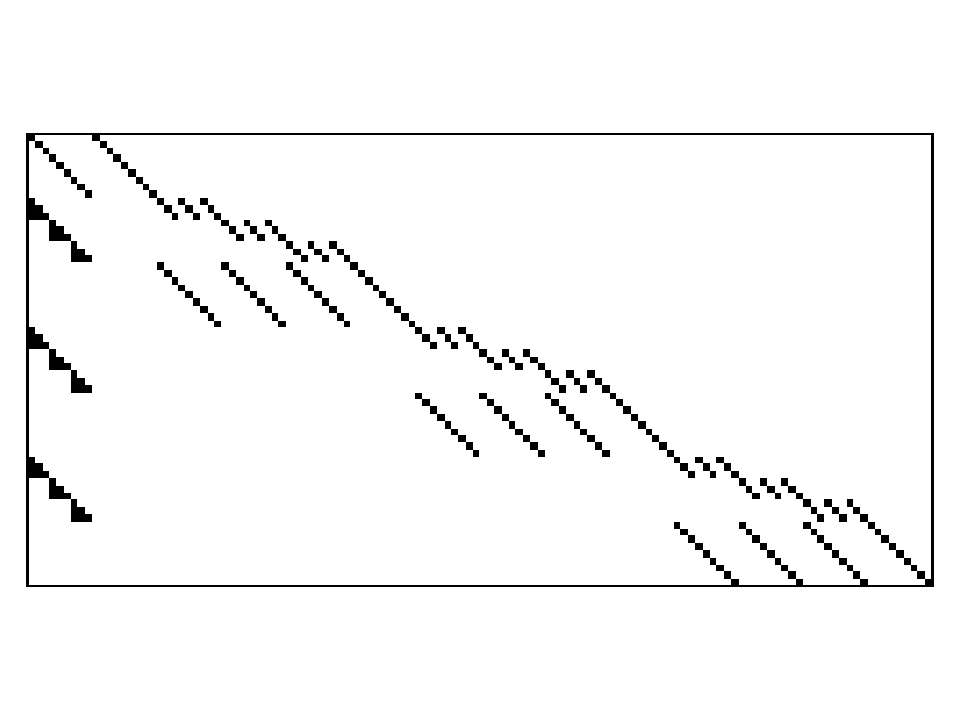
\includegraphics[width=0.45\linewidth]{DCAP_3_3_3_3}
		\label{fig:de_structure_dcap}
	}
	~
	\subfloat[][MPTSPs\_D0\_3\_3]
	{
		\centering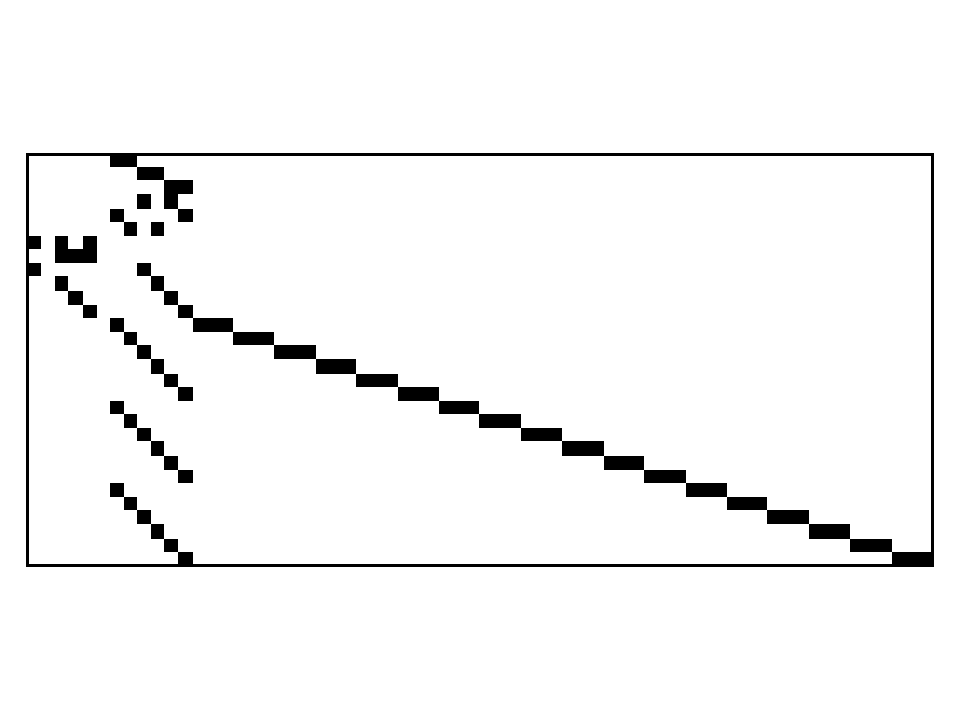
\includegraphics[width=0.45\linewidth]{MPTSPs_D0_3_3}
		\label{fig:de_structure_mptsps}
	}
	
	\subfloat[][SIZES\_3]
	{
		\centering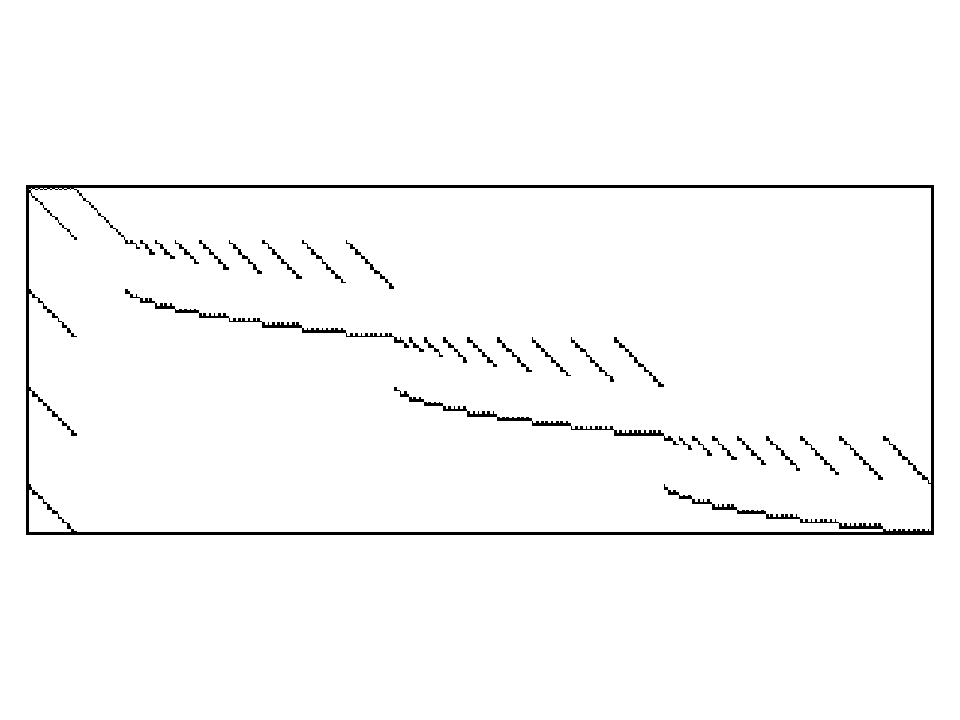
\includegraphics[width=0.45\linewidth]{SIZES_3}
		\label{fig:de_structure_sizes}
	}
	~
	\subfloat[][SMKP\_120\_3]
	{
		\centering
\includegraphics[width=0.45\linewidth]{SMKP_120_3}
		\label{fig:de_structure_smkp}
	}
	
	\subfloat[][SSLP\_5\_10\_3]
	{
		\centering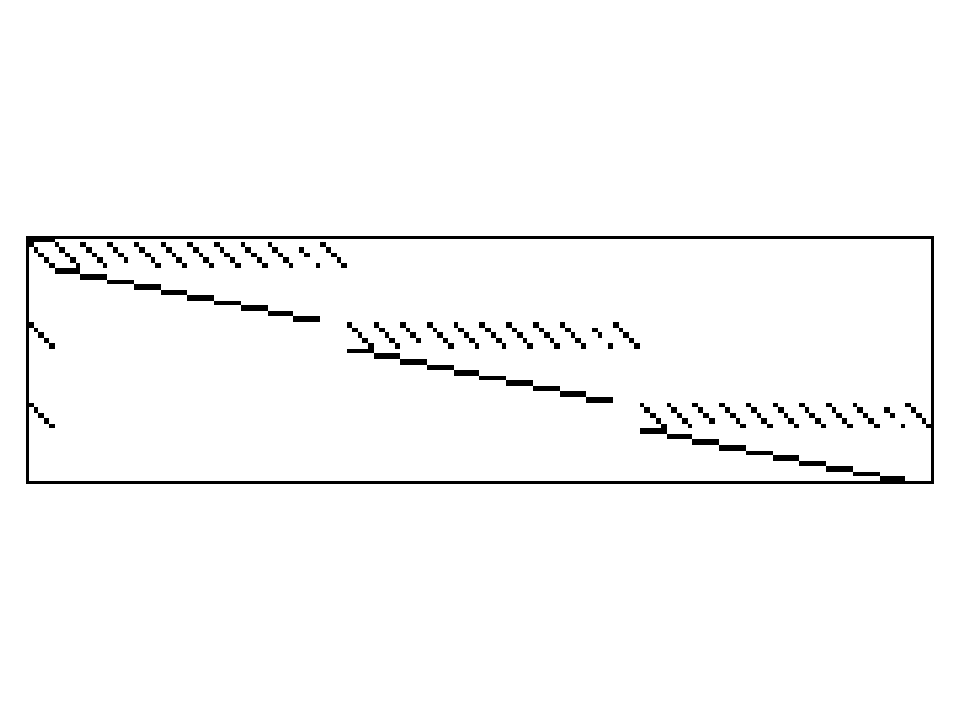
\includegraphics[width=0.45\linewidth]{SSLP_5_10_3}
		\label{fig:de_structure_sslp}
	}
	~
	\subfloat[][SUC\_FallWD\_1]
	{
		\centering
\includegraphics[width=0.45\linewidth]{SUCW_FallWD_1}
		\label{fig:de_structure_sucw}
	}

	\caption{Block-diagonal structure for each problem in extensive form}
	\begin{minipage}
		{0.65\textwidth}{\footnotesize *\texttt{SUC} instance is too huge and extremely sparse to plot more than 1 scenario}
	\end{minipage}
	\label{fig:de_structure}
\end{figure}

\begin{figure}
	\centering
	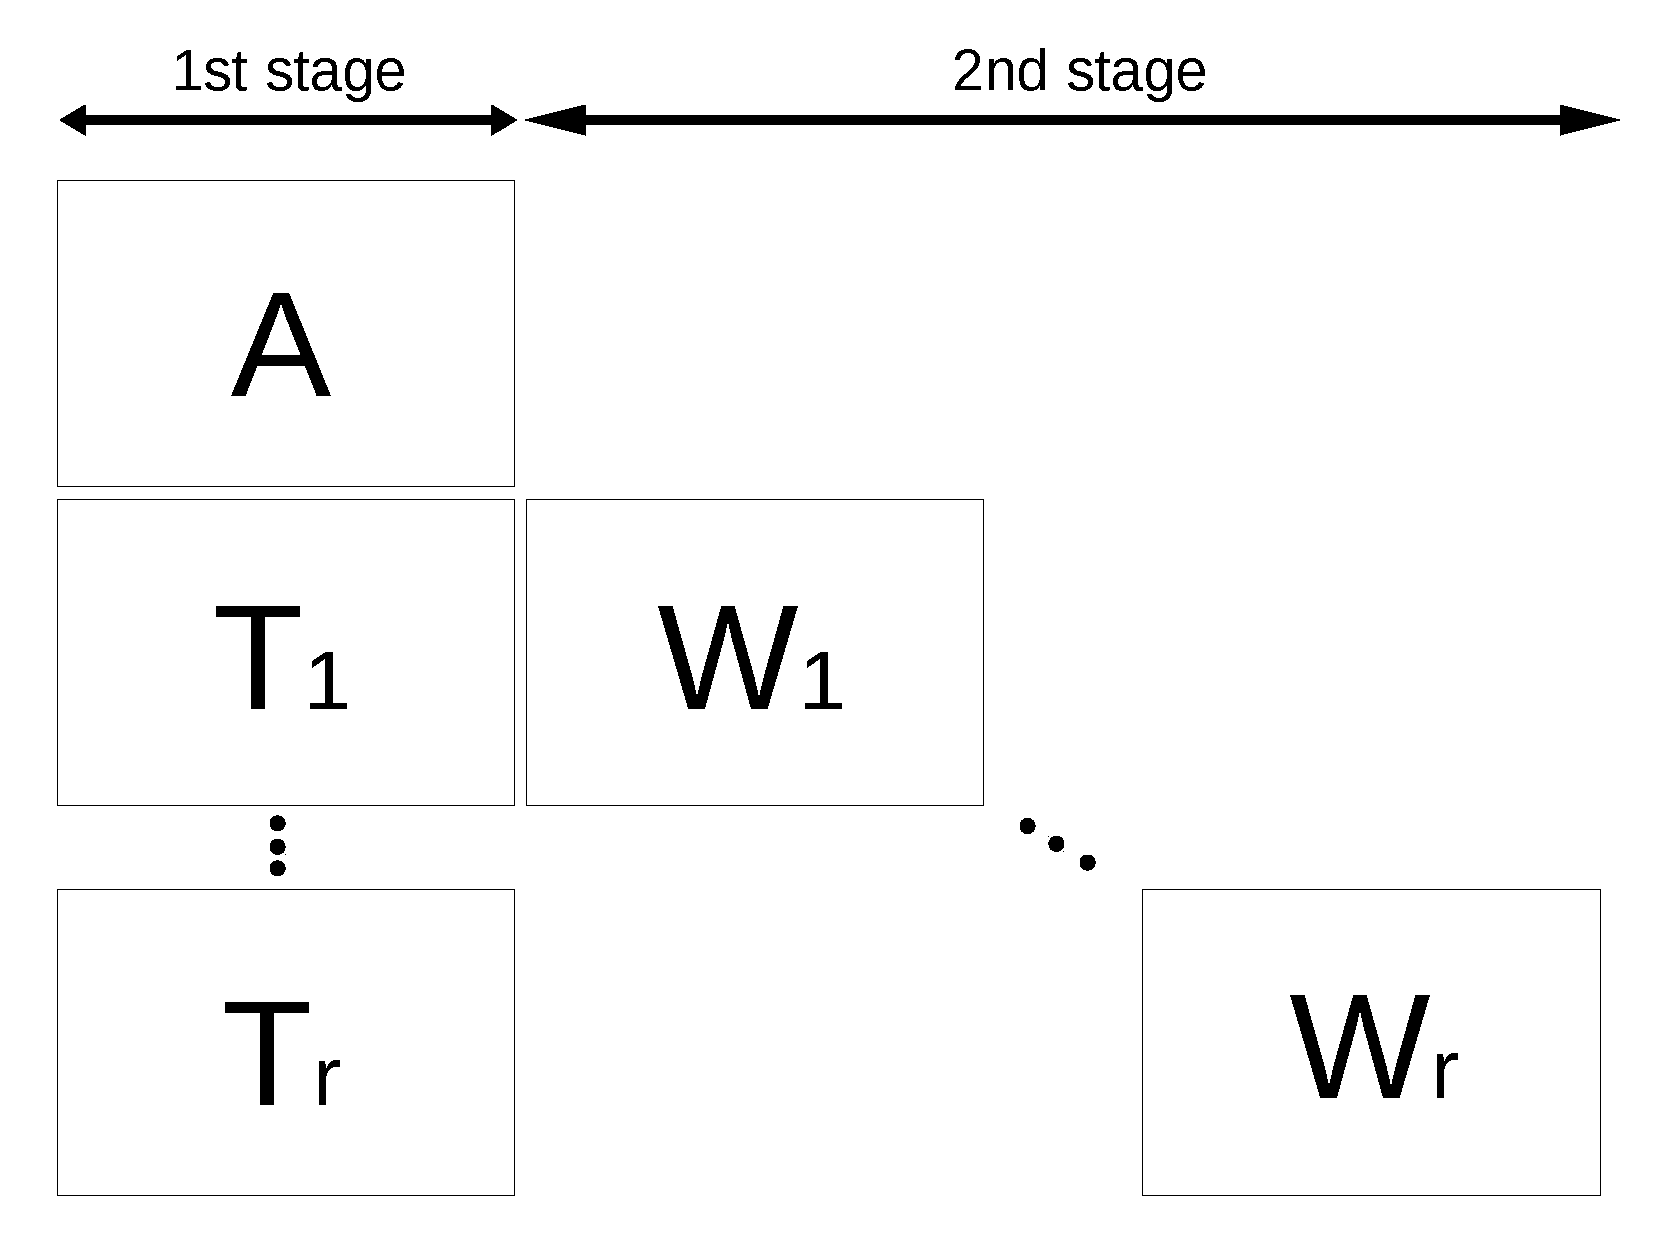
\includegraphics[width=0.7\linewidth]{drawings/stagewise_sparsity}
	\caption{Three (structurally) independent blocks in SIP}
	\label{fig:stagewise_sparsity}
\end{figure}








\pagebreak

\section{\siplibjl: A \texttt{Julia} package for \siplibtwo} \label{sec:siplibjl}
\siplibtwo\ is implemented in \julia\ programming language with algebraic modeling packages \jump\ and \structjump. We implement and provide \julia\ package, say \siplibjl, for users to utilize funtionalities of \siplibtwo. In this section, we introduce how to use \siplibjl.

\kk{An overall comment is that the minimal use of code syntax is usually good. Once the paper is published, the syntax is likely to change overtime. Then, the whole section will become wrong. For example, instead of using Siplib.jl, we can call the package or function.}
\yoc{Thanks. First of all, this section is written by benchmarking the MIPLIB 2010 paper. There is a section like this (Section 4: How to run a test, add a solver, and what the scripts do) so I think the reviewers of MPC may want us to include the section like this. And I wanted this draft to be look of completeness (not being looked abstractly) to concretely describe what is in my mind. As the main developer of SIPLIB 2.0 and based on my experience of using the Julia scripts for preliminary computational experiments, I think the current syntax I propose is reasonable and compact. The better suggestion/discussion on the syntax is always welcome and can be applied. More detailed manual will be surely accompanied later with the release of this package.} 
\kk{We may have a better idea about this section, once you start answering the questions at the end of Section 4.2. But, for now I still think it would better simply cite a github page for this kind of information.} \yoc{Okay. I first move the manual parts to Appendix. The answers for the questions at Section 4.2 will be found in Section 3.}


\subsection{\smps\ format for stochastic programming instances} \label{subsec:smps}
\smps\ format \cite{SMPS} is a data conventions for the automatic input of multiperiod stochastic linear programs. The input format is based on an old column-oriented format \mpsx\ standard and is designed to promote the efficient conversion of originally deterministic problems by introducing stochastic variants in separate files. 

Three input files are required to specify an SP in \smps\ format:
\begin{itemize}
	\item \texttt{.cor}: Core file written in \mps\ format. This describes the fundamental problem structure and contains the first-stage data and one second-stage scenario data.
	\item \texttt{.tim}: Time file which specifies the location where the 2nd stage begins.
	\item \texttt{.sto}: Stoch file which contains stochastic data of all scenarios except the one included in \texttt{.cor} file.
\end{itemize}
\kk{This needs moved to later section.} \yoc{I move this to this section.}


\pagebreak

%\section{Implementation of SmpsWriter.jl}\label{sec:smps_writer}
%We describe our Julia implementation, how to model SIP and generate SMPS files..
%\pagebreak

\section{The instance catalog: Computational benchmarks for accompanied \texttt{SMPS} files}\label{sec:instance_catalog}
%\begin{itemize}
%  \item Coin-SMI (\url{https://github.com/coin-or/Smi}): compile with CPLEX; can read SMPS and solve in extensive form.
%  \item DSP: Benders/dual decomposition
%  \item PySP: Progressive Hedging
%\end{itemize}
%
%- problem characteristics
%
%- preliminary results using CPLEX

%\kk{Please describe what you present in this section. Subsectioning would also help.} \yoc{This section is newely written. Need more justification.} 
\siplibtwo\ provides \smps\ instances for test and benchmarking  purpose. In this section, we report detailed information on each instance. This includes numerical size information, sparsity information, and computational results. The main purpose of the computational experiments is to notice 
%\begin{itemize}
%	\item Commercial MIP solver (CPLEX) result: optimality gap, integrality gap (LP relaxation gap, tightness), solution time, obj value
%	\item DD solver (DSP) result: optimality gap, duality gap (convex relaxation gap), solution time, obj value
%\end{itemize}

\subsection{Size and sparsity information}
Table \ref{table:instance_size_info} reports numerical size and sparsity information for each instance.
% Please add the following required packages to your document preamble:
% \usepackage{multirow}
% \usepackage{graphicx}
%\begin{table}[H]
%	\centering
%	\caption{Size report on the instances}
%	\label{table:instance_size_info}
%%	\resizebox{\textwidth}{!}{%
%		\Rotatebox{90}{%
%		\begin{tabular}{llrrrrrrrrrrrrrlll}
%			\hline
%			&                              & \multicolumn{3}{c}{1st stage variables} & \multicolumn{3}{c}{2nd stage variables} & \multicolumn{7}{c}{Total}                                                 & \multicolumn{3}{c}{File size}                                                  \\ \hline
%			\multicolumn{1}{c}{Problem} & \multicolumn{1}{c}{Instance} & \#cont1      & \#bin1      & \#int1     & \#cont2      & \#bin2      & \#int2     & \#cont  & \#bin    & \#int  & \#rows  & \#cols   & \#nonzeros & \%density & \multicolumn{1}{c}{.cor} & \multicolumn{1}{c}{.tim} & \multicolumn{1}{c}{.sto} \\ \hline
%			\multirow{16}{*}{DCAP}      & DCAP\_2\_3\_3\_500           & 6            & 6           & 0          & 9            & 18          & 0          & 4506    & 9006     & 0      & 7506    & 13512    & 28512      & 0.0281    &                          &                          &                          \\
%			& DCAP\_2\_3\_3\_1000          & 6            & 6           & 0          & 9            & 18          & 0          & 9006    & 18006    & 0      & 15006   & 27012    & 57012      & 0.0141    &                          &                          &                          \\
%			& DCAP\_2\_3\_3\_5000          & 6            & 6           & 0          & 9            & 18          & 0          & 45006   & 90006    & 0      & 75006   & 135012   & 285012     & 0.0028    &                          &                          &                          \\
%			& DCAP\_2\_3\_3\_10000         & 6            & 6           & 0          & 9            & 18          & 0          & 90006   & 180006   & 0      & 150006  & 270012   & 570012     & 0.0014    &                          &                          &                          \\
%			& DCAP\_2\_4\_3\_500           & 6            & 6           & 0          & 12           & 24          & 0          & 6006    & 12006    & 0      & 9006    & 18012    & 36012      & 0.0222    &                          &                          &                          \\
%			& DCAP\_2\_4\_3\_1000          & 6            & 6           & 0          & 12           & 24          & 0          & 12006   & 24006    & 0      & 18006   & 36012    & 72012      & 0.0111    &                          &                          &                          \\
%			& DCAP\_2\_4\_3\_5000          & 6            & 6           & 0          & 12           & 24          & 0          & 60006   & 120006   & 0      & 90006   & 180012   & 360012     & 0.0022    &                          &                          &                          \\
%			& DCAP\_2\_4\_3\_10000         & 6            & 6           & 0          & 12           & 24          & 0          & 120006  & 240006   & 0      & 180006  & 360012   & 720012     & 0.0011    &                          &                          &                          \\
%			& DCAP\_3\_3\_2\_500           & 6            & 6           & 0          & 6            & 18          & 0          & 3006    & 9006     & 0      & 6006    & 12012    & 25512      & 0.0354    &                          &                          &                          \\
%			& DCAP\_3\_3\_2\_1000          & 6            & 6           & 0          & 6            & 18          & 0          & 6006    & 18006    & 0      & 12006   & 24012    & 51012      & 0.0177    &                          &                          &                          \\
%			& DCAP\_3\_3\_2\_5000          & 6            & 6           & 0          & 6            & 18          & 0          & 30006   & 90006    & 0      & 60006   & 120012   & 255012     & 0.0035    &                          &                          &                          \\
%			& DCAP\_3\_3\_2\_10000         & 6            & 6           & 0          & 6            & 18          & 0          & 60006   & 180006   & 0      & 120006  & 240012   & 510012     & 0.0018    &                          &                          &                          \\
%			& DCAP\_3\_4\_2\_500           & 6            & 6           & 0          & 8            & 24          & 0          & 4006    & 12006    & 0      & 7006    & 16012    & 32512      & 0.0290    &                          &                          &                          \\
%			& DCAP\_3\_4\_2\_1000          & 6            & 6           & 0          & 8            & 24          & 0          & 8006    & 24006    & 0      & 14006   & 32012    & 65012      & 0.0145    &                          &                          &                          \\
%			& DCAP\_3\_4\_2\_5000          & 6            & 6           & 0          & 8            & 24          & 0          & 40006   & 120006   & 0      & 70006   & 160012   & 325012     & 0.0029    &                          &                          &                          \\
%			& DCAP\_3\_4\_2\_10000         & 6            & 6           & 0          & 8            & 24          & 0          & 80006   & 240006   & 0      & 140006  & 320012   & 650012     & 0.0015    &                          &                          &                          \\ \hline
%		\end{tabular}%
%%		}
%	}
%\end{table}

% Please add the following required packages to your document preamble:
% \usepackage{multirow}
% \usepackage{graphicx}
\begin{table}[H]
	\centering
	\caption{Size and sparsity report}
	\label{table:instance_size_info}
	%\resizebox{\textwidth}{!}{%
	\Rotatebox{90}{%
		\begin{tabular}{|c|l|lll|lll|lllll|llll|lll|}
			\hline
			\multicolumn{1}{|l|}{} &                               & \multicolumn{3}{c|}{1st stage variables}                                      & \multicolumn{3}{c|}{2nd stage variables (1 scenario)}                         & \multicolumn{5}{c|}{Total size}                                                                                                     & \multicolumn{4}{c|}{Sparsity}                                                                                           & \multicolumn{3}{c|}{File size}                                                  \\ \cline{3-20} 
			Problem                & \multicolumn{1}{c|}{Instance} & \multicolumn{1}{c}{cont} & \multicolumn{1}{c}{bin} & \multicolumn{1}{c|}{int} & \multicolumn{1}{c}{cont} & \multicolumn{1}{c}{bin} & \multicolumn{1}{c|}{int} & \multicolumn{1}{c}{cont} & \multicolumn{1}{c}{bin} & \multicolumn{1}{c}{int} & \multicolumn{1}{c}{rows} & \multicolumn{1}{c|}{cols} & \multicolumn{1}{c}{block A} & \multicolumn{1}{c}{block T} & \multicolumn{1}{c}{block W} & \multicolumn{1}{c|}{In total} & \multicolumn{1}{c}{.cor} & \multicolumn{1}{c}{.tim} & \multicolumn{1}{c|}{.sto} \\ \hline
			\multirow{16}{*}{DCAP} & DCAP\_2\_3\_3\_200            &                          &                         &                          &                          &                         &                          &                          &                         &                         &                          &                           &                             &                             &                             &                               &                          &                          &                           \\
			& DCAP\_2\_3\_3\_300            &                          &                         &                          &                          &                         &                          &                          &                         &                         &                          &                           &                             &                             &                             &                               &                          &                          &                           \\
			& DCAP\_2\_3\_3\_500            &                          &                         &                          &                          &                         &                          &                          &                         &                         &                          &                           &                             &                             &                             &                               &                          &                          &                           \\
			& DCAP\_2\_3\_3\_10000          &                          &                         &                          &                          &                         &                          &                          &                         &                         &                          &                           &                             &                             &                             &                               &                          &                          &                           \\
			& DCAP\_2\_4\_3\_200            &                          &                         &                          &                          &                         &                          &                          &                         &                         &                          &                           &                             &                             &                             &                               &                          &                          &                           \\
			& DCAP\_2\_4\_3\_300            &                          &                         &                          &                          &                         &                          &                          &                         &                         &                          &                           &                             &                             &                             &                               &                          &                          &                           \\
			& DCAP\_2\_4\_3\_500            &                          &                         &                          &                          &                         &                          &                          &                         &                         &                          &                           &                             &                             &                             &                               &                          &                          &                           \\
			& DCAP\_2\_4\_3\_10000          &                          &                         &                          &                          &                         &                          &                          &                         &                         &                          &                           &                             &                             &                             &                               &                          &                          &                           \\
			& DCAP\_3\_3\_2\_200            &                          &                         &                          &                          &                         &                          &                          &                         &                         &                          &                           &                             &                             &                             &                               &                          &                          &                           \\
			& DCAP\_3\_3\_2\_300            &                          &                         &                          &                          &                         &                          &                          &                         &                         &                          &                           &                             &                             &                             &                               &                          &                          &                           \\
			& DCAP\_3\_3\_2\_500            &                          &                         &                          &                          &                         &                          &                          &                         &                         &                          &                           &                             &                             &                             &                               &                          &                          &                           \\
			& DCAP\_3\_3\_2\_10000          &                          &                         &                          &                          &                         &                          &                          &                         &                         &                          &                           &                             &                             &                             &                               &                          &                          &                           \\
			& DCAP\_3\_4\_2\_200            &                          &                         &                          &                          &                         &                          &                          &                         &                         &                          &                           &                             &                             &                             &                               &                          &                          &                           \\
			& DCAP\_3\_4\_2\_300            &                          &                         &                          &                          &                         &                          &                          &                         &                         &                          &                           &                             &                             &                             &                               &                          &                          &                           \\
			& DCAP\_3\_4\_2\_500            &                          &                         &                          &                          &                         &                          &                          &                         &                         &                          &                           &                             &                             &                             &                               &                          &                          &                           \\
			& DCAP\_3\_4\_2\_10000          &                          &                         &                          &                          &                         &                          &                          &                         &                         &                          &                           &                             &                             &                             &                               &                          &                          &                           \\ \hline
		\end{tabular}%
	}
\end{table}


\subsection{Computational results}
We report computational information resulted from experiments. Unlike the size information, this information should be obtained highly computational methods. We provide the result in Table \ref{table:computation_report}. Throughout the following subsections, we explain about the computational experiments.

\subsubsection{Computing environment and setting}
All the experiments were run on \textit{Bebop}, a 1024-node computing cluster at Argonne National Laboratory \cite{bebop}. Each node in Bebop has 128GB DDR4 memory, 45MB smart cache, and Intel Xeon Processor E5-2695 v4 that consists of 18 physical cores and 36 logical threads with base processor frequency 2.10GHz and maximum turbo frequency 3.30GHz. 

We use two solvers, a commercial branch-and-cut based MIP solver \cplex\ 12.8 and an open-source DD based SIP solver \dsp. For solving master/sub problems during DD procedure in \dsp, we also use \cplex\ 12.8. We fully utilize 36 threads for each single instance both in two solvers. We set the termination condition on CPU time by 3 hours.  

The size of the instances on which the experiments perform is chosen basically based on the former \siplib. Additionally, we generate and include some large-scenario instances into the experiments.

\subsubsection{Reports}
We first introduce the notations used to define each column in the report Table \ref{table:computation_report}. The summary for the notations is found in Table \ref{table:objective-notation}.

First, recall the EF in Section \ref{sec:sip}:
\begin{subequations}\label{ef}
	\begin{align}
	\textrm{(EF) }\min_{x,y_s}\ z(x,y_s):=&\ c^{\top}x + \sum_{s=1}^{r}\PP(s) (q_j^{\top}y_s) \tag{\ref{ef:obj}}\\ 
	\mathrm{s.t.}\ &Ax\ge b,  \tag{\ref{ef:b}}\\
	&T_s x+W_s y_s\ge h_s,\quad\forall s\in\{1,\ldots,r\}, \tag{\ref{ef:c}} \\
	&x\in X, \tag{\ref{ef:d}} \\
	&y_s \in Y,\quad\forall s\in\{1,\ldots,r\}. \tag{\ref{ef:e}}
	\end{align}
\end{subequations}

We use the vanilla $z$ to denote the value of the objective function in RHS of (\ref{ef:obj}) such that constraints (\ref{ef:b})-(\ref{ef:e}) are satisfied throughout this section and report. We use the superscription $z^*$ to denote the optimal objective value, $\tilde{z}$ for the best lower bound discovered for $z^*$, and $\hat{z}$ for the incumbent objective value. Hence, the relationship $\tilde{z}\le z^*\le\hat{z}$ always holds.

$z_{LP2}$ is defined by the objective value of the following partially LP-relaxed problem:
\begin{subequations}\label{ef-lp2}
	\begin{align}
	\textrm{(EF-LP2) }\min_{x,y_s}\ z_{LP2}(x,y_s):=&\ c^{\top}x + \sum_{s=1}^{r}\PP(s) (q_j^{\top}y_s) \tag{\ref{ef:obj}}\\ 
	\mathrm{s.t.}\ &\textrm{(\ref{ef:b})}-\textrm{(\ref{ef:d})}, \nonumber \\
	& y_s \in Y \subseteq \mathbb{R}\backslash\mathbb{Z} ,\quad\forall s\in\{1,\ldots,r\}. \tag{\ref{ef:e}'}
	\end{align}
\end{subequations}
Note that only the integrality constraints for the second-stage variables are relaxed.

$z_{LD}$ is defined by the objective value of the corresponding Lagrangian dual problem. The Lagrangian dual problem can be derived from EF' (\ref{sip:ef'}) by introducing the nonanticipativity constraints (\ref{eq:SIP_2-2}) into the objective function (\ref{eq:SIP_2-1}):
\begin{subequations}\label{ef-ld}
	\begin{align}
	\textrm{(EF-LD) }\max_{\lambda\in\mathbb{R}^{r\cdot n_1}}\ z_{LD}(\lambda) :=\min_{x_s,y_s} &\sum_{s=1}^{r}p_s\left(c^{\top}x_s+q_s^{\top}y_s\right)+\lambda^\top \left(H_s x_s\right)	\tag{\ref{eq:SIP_2-1}'}\\ 
	\mathrm{s.t.}\ & (x_s,y_s)\in G_s,\quad \forall s\in\{1,\ldots,r\},	\tag{\ref{eq:SIP_2-3}}
	\end{align}
\end{subequations}
where the scenario feasibility set $G_s$ is still defined by (\ref{eq:SIP_2-4}).

\begin{table}[H]
	\centering
	\caption{Notation}
	\label{table:objective-notation}
	\resizebox{\textwidth}{!}{%
	\begin{threeparttable}
		\begin{tabular}{@{}ll@{}}
			\toprule
			Notation  & Meaning                                                                                                                    \\ \midrule
			$z$       & Objective value of EF (\ref{ef})                                                                                           \\
			$z_{LP2}$ & Objective value of EF with the second-stage only LP-relaxation (\ref{ef-lp2})                                              \\
			$z_{LD}$  & Objective value of the Lagrangian dual problem of EF (\ref{ef-ld}) \\ \bottomrule
		\end{tabular}%
				
		\begin{tablenotes}
			\small
			\item $z^*$: optimal objective value
			\item $\tilde{z}$: best lower bound for $z^*$ discovered
			\item $\hat{z}$: incumbent objective value 
		\end{tablenotes}
	\end{threeparttable}
	}
\end{table}

%\subsubsection {Basic results from the two solvers: \cplex\ and \dsp}
We report objective values from the two solvers. Since we set the time limit, the reported values can be incumbent, say, $\hat{z}_C$ and $\hat{z}_D$. When the instance is solved to the optimality in the time limit, we report the optimal objective values $z^*_C$ and $z^*_D$.

%\subsubsection{Gaps}
We report several different gaps for each instance. Each gap is useful to compare the characteristics of instances with each other. There is no guarantee that we can always obtain the optimal solution for each instance, we report the best known gaps discovered within the limited processing time (3 hours). We expect this information will provide future research direction. 


\begin{quote}
\noindent\underline{\textit{Optimality gap (OG)}} This gap, defined by, $\frac{|\underline{\hat{z}}-\hat{z}|}{|\hat{z}|+\epsilon}$, is reported from the two solvers. $\underline{\hat{z}}$ means the best lower bound discovered and $\hat{z}$ is the incumbent objective. The gap is obtained by keeping track of the best relaxation currently in the pool of nodes waiting for further processing. This can be a basic measure of difficulty of an instance combined with processing time.
\end{quote}

\begin{quote}
\noindent\underline{\textit{Integrality gap (IG)}} We define a SIP-specific integrality gap (IG) in minimization problem by $\frac{z^*}{z^*_{LP2}}$, where $z^*$ is the optimal integral solution and $z^*_{LR2}$ is the optimal fractional solution with LP-relaxed second-stage. This LP relaxation provides an optimistic bound on the integer program's solution. The small this gap implies tightness of the LP relaxation. Since there is no guarantee that we always find the optimal solutions, we report $\frac{\hat{z}}{\hat{z}_{LP2}}$ where $\hat{z}$ and $\hat{z}_{LP2}$ are the incumbent solutions. Assuming $\hat{z}_{LP2}\approxeq z^*_{LP2}$ in most cases, the reported IG will provide upper bound for the true IG. The tightness of this bound highly depends on the quality of the incumbent solution $\hat{z}$.%This gap cannot be obtained analytically so we report it based on the computational experiments.% The formulation with tighter LP relaxation is always favorable.
\end{quote}

\begin{quote}
\noindent\underline{\textit{Duality gap (DG)}} The duality gap in computational optimization is the difference between any dual objective and the incumbent primal objective. This gap also equals to the value of the convex relaxation of the primal problem. It is reported by the open-source DD solver \dsp.
\end{quote}

%\begin{quote}
%	\noindent\underline{\textit{Duality gap (DG)}} The duality gap in computational optimization is the difference between any dual solution and the value of a feasible but suboptimal iterate for the primal problem. This gap also equals to the value of the convex relaxation of the primal problem. It is reported by the open-source DD solver \dsp.
%\end{quote}

% Please add the following required packages to your document preamble:
% \usepackage{multirow}
% \usepackage{graphicx}
\begin{table}[H]
	\centering
	\caption{Computational report}
	\label{table:computation_report}
	\resizebox{\textwidth}{!}{%
		\begin{tabular}{lllllllll}
			\hline
			&                              & \multicolumn{2}{c}{Objective value (time)}          & \multicolumn{2}{c}{Optimality Gap}                  & \multicolumn{2}{c}{Integrality Gap}                 & \multicolumn{1}{c}{Duality Gap} \\ \hline
			\multicolumn{1}{c}{Problem} & \multicolumn{1}{c}{Instance} & \multicolumn{1}{c}{\cplex} & \multicolumn{1}{c}{\dsp} & \multicolumn{1}{c}{\cplex} & \multicolumn{1}{c}{\dsp} & \multicolumn{1}{c}{\cplex} & \multicolumn{1}{c}{\dsp} & \multicolumn{1}{c}{\dsp}         \\ \hline
			\multirow{16}{*}{\dcap}      & DCAP\_2\_3\_3\_200               &                           &                         &                           &                         &                           &                         &                                 \\
			& DCAP\_2\_3\_3\_300               &                           &                         &                           &                         &                           &                         &                                 \\
			& DCAP\_2\_3\_3\_500               &                           &                         &                           &                         &                           &                         &                                 \\
			& DCAP\_2\_3\_3\_10000             &                           &                         &                           &                         &                           &                         &                                 \\
			& DCAP\_2\_4\_3\_200               &                           &                         &                           &                         &                           &                         &                                 \\
			& DCAP\_2\_4\_3\_300               &                           &                         &                           &                         &                           &                         &                                 \\
			& DCAP\_2\_4\_3\_500               &                           &                         &                           &                         &                           &                         &                                 \\
			& DCAP\_2\_4\_3\_10000             &                           &                         &                           &                         &                           &                         &                                 \\
			& DCAP\_3\_3\_2\_200               &                           &                         &                           &                         &                           &                         &                                 \\
			& DCAP\_3\_3\_2\_300               &                           &                         &                           &                         &                           &                         &                                 \\
			& DCAP\_3\_3\_2\_500               &                           &                         &                           &                         &                           &                         &                                 \\
			& DCAP\_3\_3\_2\_10000             &                           &                         &                           &                         &                           &                         &                                 \\
			& DCAP\_3\_4\_2\_200               &                           &                         &                           &                         &                           &                         &                                 \\
			& DCAP\_3\_4\_2\_300               &                           &                         &                           &                         &                           &                         &                                 \\
			& DCAP\_3\_4\_2\_500               &                           &                         &                           &                         &                           &                         &                                 \\
			& DCAP\_3\_4\_2\_10000             &                           &                         &                           &                         &                           &                         &                                 \\ \hline
		\end{tabular}%
	}
\end{table}

%\begin{quote}
%\noindent\underline{\textit{Symmetry gap (SG)}} An MIP is \textit{symmetric} if its variables can be permuted without changing the structure of the problem. The symmetry is one of the frequently mentioned factors that affects the difficulty of optimization problem. Unfortunately, no universally applicable quantification for the impact of symmetry is available. Hence, we heuristically define the symmetry gap using \cplex\ option (Table \ref{table:cplex_symmetry}). That is,  
%\end{quote}

%\begin{quote}
%	\centering$\frac{|\textrm{\cplex\ solution}-\textrm{\cplex\ solution with the strongest symmetry breaking}|}{|\textrm{\cplex\ solution}|}$
%\end{quote}

%\begin{table}[H]
%	\centering
%	\resizebox{\textwidth}{!}{%
%		\begin{threeparttable}
%			\caption{Symmetry breaking option of CPLEX }
%			\label{table:cplex_symmetry}
%			\begin{tabular}{@{}cl@{}}
%				\toprule
%				Parameter value & \multicolumn{1}{c}{Meaning}                              \\ \midrule
%				-1    & Automatic: let CPLEX choose; default                     \\
%				0     & Turn off symmetry breaking                               \\
%				1     & Exert a moderate level of symmetry breaking              \\
%				2     & Exert an aggressive level of symmetry breaking           \\
%				3     & Exert a very aggressive level of symmetry breaking       \\
%				4     & Exert a highly aggressive level of symmetry breaking     \\
%				5     & Exert an extremely aggressive level of symmetry breaking \\ \bottomrule
%			\end{tabular}
%			\begin{tablenotes}
%				\small
%				\item *Parameter in \texttt{C} API is 	$\texttt{CPXPARAM\_Preprocessing\_Symmetry}$ for $>$12.6.0 and $\texttt{CPX\_PARAM\_SYMMETRY}$ for $\le$12.6.0
%			\end{tablenotes}
%		\end{threeparttable}
%	}
%\end{table}
\pagebreak

\section{Concluding remarks}\label{sec:conclusion}
\yoc{This section is newely written.}
Handling uncertainty is always complicating but unavoidable consideration in real world problems. SIP is one of the useful modeling frameworks that has been effectively addressing some of the issues. Also, unceasing efforts of researchers in this field is making great progress in terms of the range of problems that are conquered. 

Still, we believe that there are many remaining rooms to be pioneered. Since SIP can be viewed as a special case of MIP having special structure in it, they share many characteristics in common. No one can come up with the universally effective quantification of complexity both in MIP and SIP so far, however, most researchers would agree with some factors are definitely related, e.g., type of variables, size (rows and columns) of instance, and tightness/symmetry of the formulation. Some of them cannot be easily measured whereas some can be directly obtained in explicit form. We investigated each of them sometimes analytically and sometimes computationally.

In this study, we also try to provide pivotal platform as well as a milestone for further improvement in SIP by discussing the issues present in SIP and implementing convenient functionalities. Using relatively new language \julia\ hence presumably be unfamiliar, but which is most convenient and strong to the best of our knowledge, is a part of that spirit. 

Although the endemic broad viewpoint of this study restricts deeper investigation on every single different problem, we suggest researchers to dig into any one of the topics or problems more intensively. Any further contribution or suggestion for \siplibtwo\ is always welcomed. Better solution reports, more convenient functions, more interesting problems with \julia\ scripts, more effective analysis, and so on.

\kk{Writing this section would be helpful to think about what we want to present in the paper.}
\pagebreak

%\begin{acknowledgements}
%\end{acknowledgements}

\appendix
\section*{Appendix}
% problem-specific description 
In this section, we explain the meaning of the problems in \texttt{SIPLIB 2.0}. For each problem, we provide the extensive form formulation which we believe the clearest way to describe what the problem wants to do. We also give numerical parameter values together with random data generation procedures. Due to the limited access to the original data in reference papers, we sometimes selectively choose the methods from several available references and modify them without harming validity. Also, we guess some parameters about scenario generation to connect the missing links. The information in this section is completely implemented and contained in the accompanied \julia\ package: \texttt{Siplib/src/problems}. We recommend users to take a look inside the \julia\ implementation to verify the conformance of all the details.
\subsection{\airlift: Airlift operations scheduling} \label{AIRLIFT}
\airlift\ is a scheduling problem that allocates flight routes and flying number for different types of aircraft to meet uncertain cargo demands from all routes. Each aircraft type has limited number of available flying hours and different flight hours/costs. In the first stage, the number of flights and corresponding routes are initially assigned to each aircraft type. The second stage recourse action includes reallocation of flight time/route and purchase of commercial transportation. Switching aircraft from one route to another causes increased hours/costs than it is supposed to be. Moreover, it sometimes gives rise to cancellation of initially assigned flights due to the different flying ability for each type.    

Fig. \ref{fig:airlift_sparsity} shows the sparsity pattern presents in extensive form \airlift\ (single scenario).
\begin{figure}[H]
	\centering
	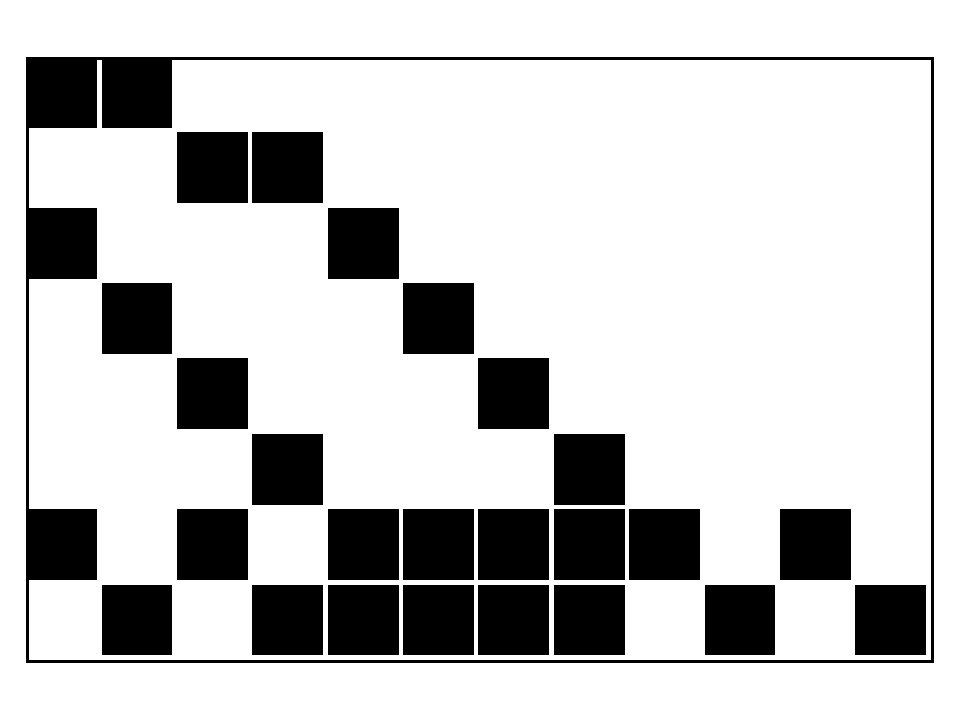
\includegraphics[width=0.85\linewidth]{AIRLIFT_1}
	\caption{AIRLIFT\_1: Extensive form constraint matrix plot}
	\label{fig:airlift_sparsity}
\end{figure}
\subsubsection{\airlift: Mathematical formulation}

\begin{subequations} \label{airlift:formulation}
	\begin{align}
	(\airlift)\ \textrm{min}\ &\sum_{i\in A}\sum_{j\in R} c_{ij}x_{ij}+\sum_{s\in\mathcal{S}}\PP(s)\Bigg[ \sum_{i\in A}\sum_{j\in R}\sum_{k\in R\backslash \{j\} }\left( \gamma_{ijk}-c_{ij}\frac{\alpha_{ijk}}{a_{ij}} \right)\chi_{ijk}^s \nonumber \\ 
	&\qquad\qquad\qquad\qquad\qquad\qquad\qquad\qquad+\sum_{j\in R}\left( c_j^+ y_j^{+s}+c_j^- y_j^{-s} \right)\Bigg]\label{airlift:obj} \\
	\textrm{s.t.}\ & \sum_{j\in R}a_{ij}x_{ij}\le F_i,\quad\forall i\in A,	\label{airlift:b}\\
	&\sum_{k\in R\backslash\{j\}}\alpha_{ijk}\chi_{ijk}^s\le a_{ij}x_{ij},\quad\forall i\in A,\ \forall j\in R,\ \forall s\in\mathcal{S}, \label{airlift:c}\\
	&\sum_{i\in A}b_{ij}x_{ij}-\sum_{i\in A}\sum_{k\in R\backslash\{j\}}b_{ij}\left(\frac{\alpha_{ijk}}{a_{ij}}\right)\chi_{ijk}^s + \sum_{i\in A}\sum_{k\in R\backslash\{j\}}b_{ij}\chi_{ikj}^s \nonumber \\
	&\qquad\qquad\qquad\qquad\qquad\quad+ y_j^{+s} - y_j^{-s} = d_j^s,\quad \forall j\in R,\ \forall s\in\mathcal{S}, \label{airlift:d}\\
	&x_{ij}\in\mathbb{Z}_+,\quad\forall i\in A,\ \forall j\in R, \\
	&\chi_{ijk}^s\in\mathbb{Z}_+,\quad\forall i\in A,\ \forall j\in R,\ \forall k\in R\backslash\{j\},\ \forall s\in\mathcal{S}, \\
	& y_j^{+s},y_j^{-s}\ge 0,\quad\forall j\in R,\ \forall s\in\mathcal{S}.
	\end{align}
\end{subequations}

\begin{table}[H]
	\caption{Notations for \airlift}
	\label{airlift:notation}
	\resizebox{\textwidth}{!}
	{
%		{@{}llp{3in}}
		\begin{tabular}{ll}
			\toprule
			\multicolumn{2}{l}{\textbf{Index sets:}} \\
			$A$ & index set of aircraft types ($i,k\in A$)\\ 
			$R$ & index set of flying routes ($j\in R$)\\ 
			$\mathcal{S}$ & index set of scenarios ($s\in \mathcal{S}$) \\ \midrule
			\multicolumn{2}{l}{\textbf{Parameters:}} \\
			$F_i$ & the maximum number of flying hours for aircraft of type $i$ available during the month\\
			$a_{ij}$ & number of hours that aircraft type $i$ requires to fly an initially assigned route $j$  \\
			$\alpha_{ijk}$ & number of hours that a re-scheduled aircraft of type $i$ requires to fly route $k$ where the initially assigned route was $j$ ($\alpha_{ijk}\ge a_{ik}$)\\
			$b_{ij}$ & carrying capacity of a flight of an aircraft type $i$ on route $j$\\
			$c_{ij}$ & cost per flight of aircraft type $i$ initially assigned to and flown on route $j$ ($c_{ij}\ge 0$)\\
			%$\gamma_{ijk} $& cost per flight of aircraft type $i$ assigned to route $k$ that uses hours made available by canceling flights on route $j$ ($\gamma_{ijk}\ge c_{ik}$)\\			
			$\gamma_{ijk} $& cost per flight of aircraft of type $i$ whose flying route is re-assigned from $j$ to $k$ ($\gamma_{ijk}\ge c_{ik}$)\\			
			$c_j^+$ & unit cost of meeting demand by commercial transport on route $j$\\
			$c_j^-$ & unit penalty cost of unused capacity on route $j$\\
			$d_j^s$ & total demand for route $j$ under scenario $s$ \\
			$\PP(s)$ & \textrm{the probability of occurence of scenario $s$} \\ \midrule
			\multicolumn{2}{l}{\textbf{Decision variables:}} \\
			$x_{ij}$ (1st-stage) & number of flights of aircraft type $i$ initially assigned to route $j$ \\
			$\chi_{ijk}^s$ (2nd-stage) & number re-scheduled flights of aircraft type $i$ from route $j$ to $k$ \\ 
			$y_j^{+s}$ (2nd-stage) & amount of demand carried by commercial transportation on route $j$ under scenario $s$\\
			$y_j^{-s}$ (2nd-stage) & amount of unused capacity on route $j$ under scenario $s$\\
			\bottomrule
		\end{tabular}
	}
\end{table} 

\subsubsection{\airlift: Data generation}
The original reference \cite{journal:MW1969} provides a numerical example with $|A|=2$ and $|R|=2$ (Table \ref{AIRLIFT:numeric}). 

\begin{table}[H]
	\caption{\airlift: Numerical data in \cite{journal:MW1969}}
	\label{AIRLIFT:numeric}
	\centering
	\resizebox{\textwidth}{!}{%
		\begin{tabular}{cccccccccccc}
			\hline
			\multirow{2}{*}{\begin{tabular}[c]{@{}c@{}}Aircraft \\ type $(i)$\end{tabular}} & \multicolumn{2}{c}{$a_{ij}$ (hours)} & \multicolumn{2}{c}{$b_{ij}$ (tons)} & \multicolumn{2}{c}{$c_{ij}$ (dollars)} & $\alpha_{ijk}-a_{ij}$ (hours) & $\gamma_{ijk}-c_{ij}$ (dollars) & \multicolumn{2}{c}{$c_j^+$ (dollars)}       & $c_j^-$ (dollars)\$ \\ \cline{2-12} 
			& $j=1$             & $j=2$            & $j=1$            & $j=2$            & $j=1$              & $j=2$             & $\forall (j,k)$               & $\forall (j,k)$                 & $j=1$                & $j=2$                & $j=1,2$             \\ \hline
			1                                                                               & 24                & 14               & 50               & 75               & 7200               & 6000              & 5                             & 1000                            & \multirow{2}{*}{500} & \multirow{2}{*}{250} & \multirow{2}{*}{0}  \\
			2                                                                               & 49                & 29               & 20               & 20               & 7200               & 4000              & 7                             & 1500                            &                      &                      &                     \\ \hline
		\end{tabular}%
	}
\end{table}
According to the original reference, demand on each route is lognormally distributed with mean and standard deviation pairs (1000, 50) and (1500, 300). To get the desired result, we generate random numbers from the following lognormal distributions:
\begin{align*}
d_1^s&=Lognormal(\mu=6.906,\ \sigma=0.05),\quad\forall s\in\mathcal{S},\\
d_2^s&=Lognormal(\mu=7.2936,\ \sigma=0.198),\quad\forall s\in\mathcal{S}.
\end{align*}

\subsection{\dcap: Dynamic capacity planning with stochastic demand} \label{DCAP}
\dcap\ is the problem of determining a capacity expansion schedule for a set of resources, and the assignment of resource capacity to task with stochastic requirement over a multi-period planning horizon. We refer to the main reference \cite{journal:AG2004}.

Fig. \ref{fig:dcap_sparsity} shows the sparsity pattern presents in extensive form \dcap\ (single scenario).
\begin{figure}[H]
	\centering
	
\includegraphics[width=\linewidth]{DCAP_3_3_3_1}
	\caption{DCAP\_3\_3\_3\_1: Extensive form constraint matrix plot}
	\label{fig:dcap_sparsity}
\end{figure}
%In \texttt{SIPLIB}, 12 instances are available in \texttt{SMPS} format with the largest instance comprises of 500 scenarios correspond to the size of 9,012 rows and 18,018 columns. 

%\dcap\ is a problem of deciding the capacity expansion schedule for $m$ resources over $T$ time periods in order to satisfy the processing requirements of $n$ tasks.
\subsubsection{\dcap: Mathematical formulation}
We consider the problem of deciding the capacity expansion schedule for $|R|$ resources over $|T|$ time periods to satisfy the processing requirements of $|N|$ tasks where $R$, $T$, and $N$ denote set of resources, set of time periods, and set of tasks, respectively. We define decision variables: the first-stage continuous variable $x_{it}$ for the capacity acquisition of resource $i$ in period $t$ and the second-stage binary variable $y_{ijt}^s$ to indicate whether resource $i$ is assigned to task $j$ in period $t$ under scenario $s$. Additional first-stage binary variable $u_{it}$ is for logical constraint whether or not we decided to acquire more capacity of resource $i$ in period $t$. Hence, for all resource $i\in R$ and time $t\in T$, $u_{it}=1$ if $x_{it}>0$, $u_{it}=0$ otherwise. 

Under the definition of the decision variables, the extensive form of \dcap\ is written below and the summarized notation is available in Table \ref{dcap:notation}.

\begin{subequations} \label{dcap:formulation}
	\begin{align}
	(\dcap)\ \textrm{min}\ &\sum_{t\in T}\sum_{i\in R}\left(\alpha_{it}x_{it}+\beta_{it}u_{it}\right)+\sum_{s\in\mathcal{S}}\PP(s)\sum_{t\in T}\sum_{i\in R\cup\{0\}}\sum_{j\in N}c_{ijt}^{s}y_{ijt}^s	\label{dcap:obj} \\
	\textrm{s.t.}\ & x_{it}\le \textrm{M}u_{it},\quad\forall i\in R,\ \forall t\in T,	\label{dcap:b}\\
	&\sum_{j\in N}d_{jt}^s y_{ijt}^s\le\sum_{\tau=1}^{t}x_{i\tau},\quad\forall i\in R,\ \forall t\in T,\ \forall s\in\mathcal{S},\label{dcap:c}\\
	&\sum_{i\in R\cup \{0\}}y_{ijt}^s=1,\quad\forall j\in N,\ \forall t\in T,\ \forall s\in\mathcal{S}, \label{dcap:d} \\
	&x_{it}\ge 0,\quad\forall i\in R,\ \forall t\in T,\label{dcap:e} \\
	&u_{it}\in\{0,1\}, \quad\forall i\in R,\ \forall t\in T,\label{dcap:f}\\
	&y_{ijt}^s\in\{0,1\},\quad\forall i\in R\cup\{0\},\ \forall j\in N,\ \forall t\in T,\ \forall s\in\mathcal{S},\label{dcap:g}
	\end{align}
\end{subequations}
The objective function (\ref{dcap:obj}) is to minimize total expected cost for the capacity expansion schedule. The first double summation denotes the expansion cost for resource $i$ in period $t$ where $\alpha_{it}$ and $\beta_{it}$ are the variable and fixed cost, respectively. The second term in the objective function represents the expected assignment cost in period $t$ over all scenario $s\in\mathcal{S}$. Note that a dummy resource $i=0$ is included with infinite capacity. The cost $c_{0jt}^s$ denotes the penalty of failing to assign a resource to task $j$. The dummy resource enforces the \textit{complete recourse property}, which ensures that there is a feasible second-stage assignment in all periods and all scenarios for any capacity acquisition schedule \cite{journal:AG2004}. Constraint (\ref{dcap:b}) is the logical constraint containing a suitably large value M (we set M=1 in \siplibtwo\ to follow the original implementation in \siplib\, although it does not seem to be large enough) to define the cost for capacity expansion. Constraint (\ref{dcap:c}) reflects that the processing requirement of all tasks assigned to a resource in any period cannot exceed the installed capacity in that period under all scenarios. Constraint (\ref{dcap:d}) guarantees that each task needs to be assigned to exactly one resource in each period under all scenarios. Finally, constraints (\ref{dcap:e})-(\ref{dcap:g}) restrict the space from which the variables take values.

\begin{table}[H]
	\caption{Notations for \dcap}
	\label{dcap:notation}
	\resizebox{\textwidth}{!}
	{
		\begin{tabular}{ll}
			\toprule
			\multicolumn{2}{l}{\textbf{Index sets:}} \\
			$R$ & index set of resources ($i\in R\cup\{0\}$ where $0$ is a dummy resource with infinite capacity) \\ 
			$N$ & index set of tasks ($j\in N$)\\ 
			$T$ & index set of time periods ($t\in T$)\\
			$\mathcal{S}$ & index set of scenarios ($s\in \mathcal{S}$) \\ \midrule
			\multicolumn{2}{l}{\textbf{Parameters:}} \\
			$\alpha_{it}$ & variable cost for expanding capacity of resource $i$\\ 
			$\beta_{it}$ & fixed cost for expanding capacity of resource $i$ \\ 
			$c_{ijt}^{s}$ & cost of processing task $j$ using resource $i$ in period $t$ under scenario $s$ \\ 
			$d_{jt}^s$	& processing requirement for task $j$ in period $t$ under scenario $s$		\\
			$\PP(s)$ & \textrm{the probability of occurence of scenario $s$} \\ \midrule
			\multicolumn{2}{l}{\textbf{Decision variables:}} \\
			$x_{it}$ (1st-stage) & capacity acquisition amount of resource $i$ in period $t$ \\ 
			$u_{it}$ (1st-stage)& 1 if capacity of resource $i$ is expanded in period $t$, 0 otherwise \\ 
			$y_{ijt}^s$ (2nd-stage)& 1 if resource $i$ is assigned to task $j$ in period $t$ under scenario $s$, 0 otherwise\\
			\bottomrule
		\end{tabular}
	}
\end{table} 

\subsubsection{\dcap: Data generation} \label{subsubsec:dcap_data_gen}
There are four factors that define the instance of \dcap: $|R|$, $|N|$, $|T|$, and $|\mathcal{S}|$. Once we decide the factors, the instance is named by DCAP\_$|R|$\_$|N|$\_$|T|$\_$|\mathcal{S}|$. Let $U$ be a continuous uniform random variable: $U\sim Unif(0,1)$. Then, the parameters are generated as follows:
\begin{align*}
	\alpha_{it}&=5U+5,\quad\forall i\in R,\ \forall t\in T, \\
	\beta_{it} &=40U+10,\quad\forall i\in R,\ \forall t\in T, \\
	c_{ijt}^s  &=5U+5,\quad\forall i\in R,\ \forall j\in N,\ \forall t\in T,\ \forall s\in\mathcal{S}, \\
	c_{0jt}^s  &=500U+500,\quad\forall j\in N,\ \forall t\in T,\ \forall s\in\mathcal{S}, \\
	d_{jt}^s   &=U+0.5,\quad\forall j\in N,\ \forall t\in T,\ \forall s\in\mathcal{S}.
\end{align*}

\subsection{\mptsps: Mutli-path traveling salesman problem with stochastic travel times} \label{MPTSPs}
\mptsps\ is a variant of the travelling salesman problem (TSP) where a set of paths exists between any two nodes and each path is characterized by a random travel time. 

In \siplib, only limited data (e.g., number of nodes, coordinates of nodes, generated travel times) are provided and no \smps\ file is available. We mainly refer to \cite{journal:PGM2017} for deriving the mathematical formulation. Due to the malfunction of subtour breaking constraints in the reference model, we refer to another paper \cite{journal:LSD1990} to contain working subtour-breaking constraint.

Fig. \ref{fig:mptsps_sparsity} shows the sparsity pattern presents in extensive form \mptsps\ (single scenario).
\begin{figure}[]
	\centering
	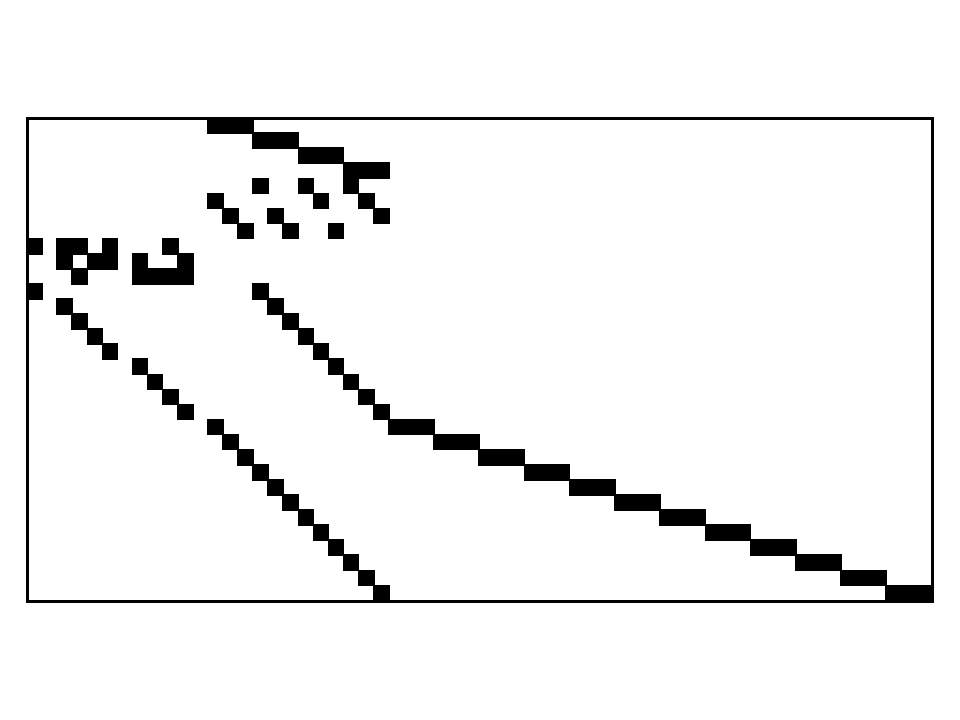
\includegraphics[width=\linewidth]{MPTSPs_D0_4_1}
	\caption{MPTSPs\_D0\_4\_1: Extensive form constraint matrix plot}
	\label{fig:mptsps_sparsity}
\end{figure}

 %Combining the two references, we construct the forthcoming single commodity flow-based formulation \mptsps\ that is used for \siplibtwo. 
\subsubsection{\mptsps: Mathematical formulation}
We consider a two-stage SIP with recourse. The travel time oscillation $e_{ij}^k$ by using path $k$ between nodes $i$ and $j$. We present each realization (scenario) of random travel time oscillation by $e_{ijk}^{s}$ where $s$ indicates the scenario. In \mptsps\, at the first stage, the decision-maker does not have any information about the travel time oscillation. The tour paths among the nodes, however, should be determined before the complete information is available. The first stage decision variable $y_{ij}$ is represented by the selection of nodes $i$ and $j$ to be visited in a tour. In the second stage where the random travel time $c_{ijk}^{s}$ are available, the paths $k$ between each couple of nodes $i$ and $j$ under scenario $s$, $x_{ijk}^{s}$ can be calculated. 

Let $N$ and $K_{ij}$, respectively, be the finite set of nodes of the graph and the set of paths between the pair of nodes $i,j\in N$. We denote with $\mathcal{S}$ the set of scenarios with associated equally distributed probability of each scenario $\PP(s)$, i.e., $\PP(s)\equiv 1/|\mathcal{S}|$. Each path $k\in K_{ij}$ between nodes $i,j\in N$ is characterized by a non-negative estimation of the mean unit travel time $\bar{c}_{ij}$ and a non-negative unit random travel time $c_{ijk}^{s}$ under the scenario $s\in S$. Let $e_{ijk}^{s}\equiv c_{ijk}^{s}-\bar{c}_{ij}$ be the error on the travel time estimated for the path $k\in K_{ij}$ under time scenario $s\in S$.

The first stage binary variables $y_{ij}=1$ if node $j\in N$ is visited right after node $i\in N$, 0 otherwise. The second stage binary variables $x_{ijk}^{s}=1$ if path $k\in K_{ij}$ between nodes $i,j\in N$ is selected at the second stage, 0 otherwise. We have one more set of first stage variables $\phi_{ij}$ which is introduced to break the subtours \cite{journal:LSD1990}. The non-negative continuous variables $\phi_{ij}$ describe the flow of a single commodity to node 1 from every other nodes (without loss of generality, 1 is the starting node). 

The extensive form of \mptsps\ is as follows and the notations used are summarized in Table \ref{mptsps:notation}.
\begin{subequations} \label{mptsps:formulation}
	\begin{align}
	(\mptsps)\ \textrm{min}\ &\sum_{i\in N}\sum_{j\in N\backslash\{i\}}\bar{c}_{ij}y_{ij}+\sum_{s\in \mathcal{S}}\PP(s)\sum_{i\in N}\sum_{j\in N\backslash\{i\}}\sum_{k\in K_{ij}}e_{ijk}^{s}x_{ijk}^{s} \label{mptsps:obj} \\ 
	\textrm{s.t.}\ &\sum_{j\in N\backslash\{i\}}y_{ij}=1,\quad\forall i\in N, \label{mptsps:con1} \\ 
	&\sum_{i\in N\backslash\{j\}}y_{ij}=1,\quad\forall j\in N,\label{mptsps:con2} \\ 
	&\sum_{j\in N}\phi_{lj}-\sum_{i\in N\backslash\{1\}}\phi_{il}=1,\quad\forall l\in N\backslash\{1\}, \label{mptsps:con3}  \\ 
	&\phi_{ij}\le \left(|N|-1\right)y_{ij},\quad\forall i\in N\backslash\{1\},\ \forall j\in N\backslash\{i\}, \label{mptsps:con4} \\ 
	&\sum_{k\in K_{ij}}x_{ijk}^{s}=y_{ij},\quad\forall i\in N,\ \forall j\in N\backslash\{i\},\ \forall s\in \mathcal{S}, \label{mptsps:con5} \\ 
	&y_{ij}\in \{0,1\},\quad \forall i\in N,\ \forall j\in N\backslash\{i\}, \label{mptsps:con6} \\ 
	&\phi_{ij} \ge 0, \quad \forall i\in N\backslash\{1\},\ \forall j\in N. \label{mptsps:con7} \\
	&x_{ijk}^{s}\in\{0,1\},\quad\forall i\in N,\ \forall j\in N\backslash\{i\},\ \forall k\in K_{ij},\ \forall s\in \mathcal{S}, \label{mptsps:con8} 
	\end{align}
\end{subequations}
The first sum in the objective function (\ref{mptsps:obj}) represents the first stage travel cost, while the second sum represents the recourse action, consisting in choosing the best path $k\in K_{ij}$ under scenario $s\in\mathcal{S}$. The constraints (\ref{mptsps:con1}) and (\ref{mptsps:con2}) form the assignment constraints and ensure that each node is visited only once. Given the fixed values of $y_{ij}$, constraint (\ref{mptsps:con3}) and (\ref{mptsps:con4}) form a network flow problem, and therefore the $\phi_{ij}$ values will be integer. In case the solutions of the above formulation contain at least one subtour, the constraints (\ref{mptsps:con3}) and (\ref{mptsps:con4}) are violated. Moreover, no tour can exist that does not contain node 1 by the two constraints. For more explanation on the subtour breaking mechanism accompanied with rigorous proof, refer to \cite{GG1978}. The constraint (\ref{mptsps:con5}) guarantees that path $k$ between nodes $i$ and $j$ can be chosen at stage 2 only if nodes $i$ and $j$ were part of the tour fixed at stage 1. Finally, the constraints (\ref{mptsps:con6})-(\ref{mptsps:con8}) restrict the space from which the variables take values.

\begin{table}[H]
	\caption{Notations for \mptsps}
	\label{mptsps:notation}
	\resizebox{\textwidth}{!}
	{
		\begin{tabular}{ll}
			\toprule
			\multicolumn{2}{l}{\textbf{Index sets:}} \\
			$N$ & \textrm{index set of nodes ($i,j,l\in N$)} \\ 
			$K_{ij}$ & \textrm{index set of paths between nodes $i$ and $j$ ($k\in K_{ij}$)} \\ 
			$\mathcal{S}$ & \textrm{index set of scenarios ($s\in \mathcal{S}$)}\\ \midrule
			\multicolumn{2}{l}{\textbf{Parameters:}} \\
			$c_{ijk}^{s}$ & \textrm{unit random travel time of path $k$ between nodes $i,j$ under scenario $s$} \\ 
			$\bar{c}_{ij}$ & \textrm{estimation of the mean unit travel time (expectation of $c_{ijk}^{s}$ over all $s$ and $k$)} \\ 
			$e_{ijk}^{s}$ & \textrm{the error on the travel time on estimated for arc $(i,j)$ and path $k$ under scenario $s$} \\ 
			$\PP(s)$ & \textrm{the probability of occurence of scenario $s$} \\  \midrule
			\multicolumn{2}{l}{\textbf{Decision variables:}} \\
			$\phi_{ij}$ (1st-stage) & \textrm{the nonnegative real-valued flow on arc $(i,j)$}\\
			$y_{ij}$ (1st-stage)& \textrm{1 if path $k$ between nodes $i,j\in N$ is selected at the second-stage, 0 otherwise} \\  
			$x_{ijk}^{s}$ (2nd-stage) & \textrm{1 if node $j$ is visited just after node $i$, 0 otherwise} \\ 
			\bottomrule
		\end{tabular}
	}
\end{table} 


\subsubsection{\mptsps: Data generation} \label{mptsps:datagen}
We follow the scenario generation methods described through the references \cite{journal:MPT2014,journal:PGM2017,journal:TPP2017}. For \mptsps\, there are three mainly distinguished characteristics for each instance: the nodes partition strategy ($D\in\{D0,D1,D2,D3\}$, explanation on each strategy is forthcoming), the number of nodes ($|N|\in\{2,3,\ldots\}$), and the number of scenarios ($|\mathcal{S}|\in\{1,2,\ldots\}$). Another important charicteristic $|K_{ij}|\in\{1,2,3,\ldots\}$ is the number of paths for each edge which is fixed by 3 as a default following \cite{journal:TPP2017}. Once we decide $D$, $|N|$, and $|S|$ by, each instance is named by MPTSPs\_$D$\_$|N|$\_$|\mathcal{S}|$.

The nodes are distributed in a circle with radius equal to $r$ km. We use Cartesian coordinate system where the geometric center of the circle is $(r,r)$. The nodes are distinguished by two subsets: \textit{central} and \textit{suburban}. If the Euclidean distance between a node and the geometric center is less than or equal to the half of the radius ($r/2$), then the node is of \textit{central} type. Otherwise, if the Euclidean distance is greater than the half of the radius, the node is of \textit{suburban} type. Each arc between any two nodes $i$ and $j$ is either \textit{homogeneous} or \textit{heterogeneous}. If the two nodes are of the same type of node, i.e., both are \textit{central} or both are \textit{suburban}, the type of the arc is \textit{homogeneous}. Otherwise, the type of the arc is \textit{heterogeneous}. Later, the travel time of each path between two nodes are affected by the type of arc. 

The nodes are generated by one of the following distribution strategies:
\begin{itemize}
	\item $D0$: All the nodes are \textit{central}.
	\item $D1$: All the nodes are \textit{suburban}.
	\item $D2$: 3/4 of the nodes are \textit{central} and the remaining 1/4 are \textit{suburban}.
	\item $D3$: 1/2 of the nodes are \textit{central} and the remaining 1/2 are \textit{suburban}.
\end{itemize}

Given $D,|N|$ and $|\mathcal{S}|$, the next procedure can be summarized as follows:
\begin{enumerate}
	\item Generate $|N|$ nodes based on the predetermined strategy $D$. Then, the nodes are generated by acceptance-rejection procedure with uniform random number generation. Again following \cite{journal:TPP2017}, we fix $r=7$\textit{km}. 
	\item Calculate Euclidean distances between the nodes ($EC_{ij}$).
	\item We guess and fix the deterministic velocity profile by 40\textit{km/h} for the \textit{central} nodes and 80\textit{km/h} for the \textit{suburban} nodes: $v_{cntr}=40$ and $v_{sbrb}=80$.
	\item Generate random travel times ($c_{ijk}^{s}$) for each scenario $s$.
	\begin{itemize}
		\item The velocity for traveling arc $(i,j)$ is affected by its arc type.
		%\item Each arc has $|K_{ij}|$ paths (we have fixed it $|K_{ij}|=3$ for all $i,j$).
		\item If the arc is \textit{homogeneous}, the random travel time of all the paths are generated only based on the corresponding velocity profile.
		\item If the arc is \textit{heterogeneous}, $\ceil*{\frac{|K_{ij}|}{3}}$ paths are generated based on $v_{cntr}=40$ and the remaining paths are generated based on $v_{sbrb}=80$. 
		\item The velocities are distributed by $Unif(\frac{v}{2},2v)$ for $v=v_{cntr},v_{sbrb}$.
		\item In summary, if the arc $(i,j)$ is \textit{homogeneous}, 
		\begin{align*}
		c_{ijk}^{s}\sim\left\{ \begin{array}{ll} \frac{EC_{ij}}{Unif(\frac{v_{cntr}}{2},2v_{cntr})} & \textrm{if $i,j$ are both \textit{central},} \\
		\frac{EC_{ij}}{Unif(\frac{v_{sbrb}}{2},2v_{sbrb})} & \textrm{if $i,j$ are both \textit{suburban},}	\end{array} \right.\ \forall k\in K_{ij}.
		\end{align*}
		\item Otherwise, if $(i,j)$ is \textit{heterogeneous},
		\begin{align*}
		c_{ijk}^{s}\sim\left\{ \begin{array}{ll} \frac{EC_{ij}}{Unif(\frac{v_{cntr}}{2},2v_{cntr})} & \textrm{for $k\in\left\{1,\ldots,\ceil*{\frac{|K_{ij}|}{3}}\right\}$,} \\
		\frac{EC_{ij}}{Unif(\frac{v_{sbrb}}{2},2v_{sbrb})} & \textrm{for $k\in\left\{\ceil*{\frac{|K_{ij}|}{3}}+1,\ldots,|K_{ij}|\right\}$.}	\end{array} \right.
		\end{align*}
	\end{itemize}
	\item Finally, we multiply 3600 for each component of $c_{ijk}^{s}$ to convert the unit from \textit{hours} to \textit{seconds}.
\end{enumerate}


\subsection{\sdcp: Stochastic data center placement} \label{SDCP}
The stochastic data center placement (SDCP) problem is to find the optimal placement of data centers (as dispatchable loads) that minimizes the expected total electricity dispatch cost over stochastic wind power generation scenarios. We refer to \cite{journal:KYZC2017} for mathematical models. For model parameters, we use Western Electricity Coordinating Council data set (WECC \cite{web:wecc}) interconnected with California ISO Open Access Same-Time Information System (CAISO) as in the reference. 

Fig. \ref{fig:sdcp_sparsity} shows the sparsity pattern presents in extensive form \sdcp\ (single scenario).
\begin{figure}[H]
	\centering
	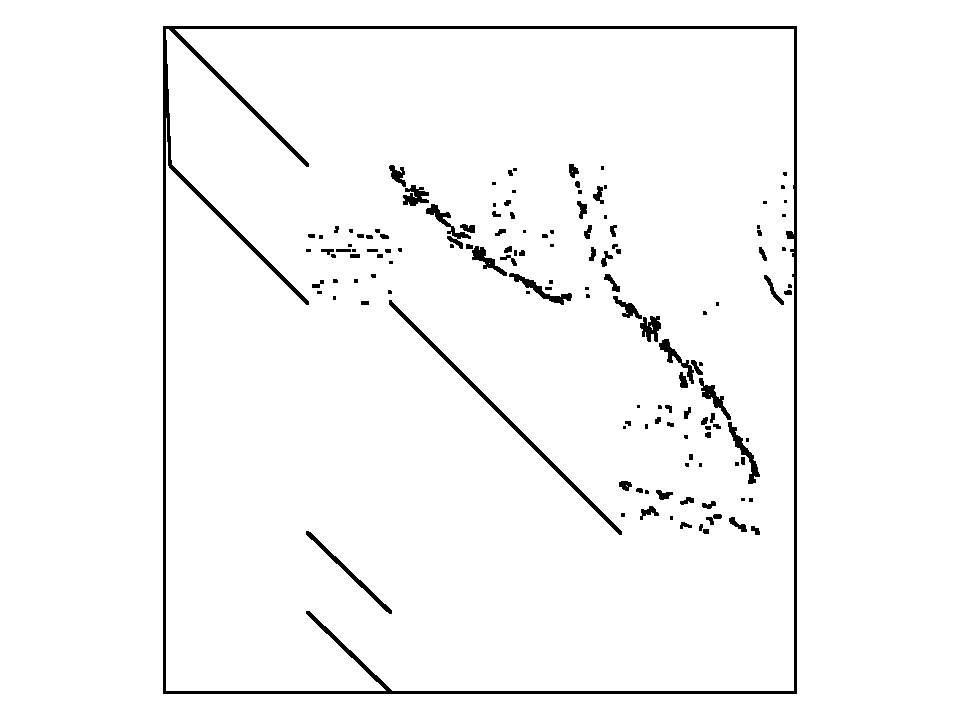
\includegraphics[width=\linewidth]{SDCP_5_10_FallWD_1}
	\caption{SDCP\_5\_10\_FallWD\_1: Extensive form constraint matrix plot}
	\label{fig:sdcp_sparsity}
\end{figure}

\subsubsection{\sdcp: Mathematical formulation}
In \sdcp, we make a here-and-now decision on the number and locations of data centers to be installed at location (bus) $n\in N$ at the first stage. In the second stage, the minimal cost recourse decision to dispatch loads and electricity is made considering wind power generation scenarios. The dispatching decision involves flows, angles, supply, loads, and spillages.

Using the notation in Table \ref{sdcp:notation}, the extensive form of \sdcp\ can be stated as in the following model \ref{sdcp:formulation}.
\begin{subequations} \label{sdcp:formulation}
	\begin{align}
	(\sdcp)\ \textrm{min}\ &\sum_{s\in\mathcal{S}}\PP(s)\sum_{t\in T} 
	\Bigg[\sum_{g\in G}C_g p_{gts} + \sum_{\lambda\in \mathcal{L}} C^{\mathcal{L}}x_{\lambda ts}^{\mathcal{L}} \nonumber \\&\qquad\qquad\qquad\qquad\qquad + \sum_{\iota\in \mathcal{I}} C^{\mathcal{I}}x_{\iota ts}^{\mathcal{I}} + \sum_{\rho\in \mathcal{R}} C^{\mathcal{R}}x_{\rho ts}^{\mathcal{R}} + \sum_{\omega\in \mathcal{W}} C^{\mathcal{W}}x_{\omega ts}^{\mathcal{W}} \Bigg]
	\label{sdcp:obj}\\
	\textrm{s.t.}\ &  \textrm{(First-stage constraints)} \nonumber\\
	&\sum_{n\in N} d_n \le K,\label{sdcp:b}\\
	&\textrm{(Second-stage constraints)} \nonumber\\
	&u_{nts} \le Ud_n,\quad\forall n\in N,\ \forall t\in T,\ \forall s\in\mathcal{S},\label{sdcp:c}\\
	&\sum_{l\in L_n^+}f_{lts}-\sum_{l\in L_n^-}f_{lts}+\sum_{g\in G_n}p_{gts}+\sum_{\iota\in IG_n^\mathcal{I}}\left(IC_{\iota t}^\mathcal{I}-x_{\iota ts}^\mathcal{I}\right)\nonumber\\
	&+\sum_{\omega\in IG_n^\mathcal{W}}\left(IC_{\omega ts}^\mathcal{W}-x_{\omega ts}^\mathcal{W}\right)
	+\sum_{\rho\in IG_n^\mathcal{R}}\left(IC_{\rho t}^\mathcal{R}-x_{\rho ts}^\mathcal{R}\right)
	-u_{nts} \nonumber\\
	&=\sum_{\lambda\in IG_n^\mathcal{L}}\left(IC_{\lambda t}^\mathcal{L}-x_{\lambda ts}^\mathcal{L}\right),\quad\forall n\in N,\ \forall t\in T,\ \forall s\in\mathcal{S},\label{sdcp:d}\\
	&f_{lts}=B_l\left(  \theta_{n_1 ts}-\theta_{n_2 ts}  \right),\quad\forall l\equiv (n_1, n_2)\in L,\ t\in T, s\in\mathcal{S},\label{sdcp:e}\\
	&-R_g^- \le p_{gts}-p_{g,t-1,s} \le R_g^+ ,\quad\forall g\in G,\ \forall t\in T,\ \forall s\in\mathcal{S},\label{sdcp:f}\\
	&  \textrm{(First-stage variable bounds)} \nonumber\\
	&d_n \in \mathbb{Z}_+,\quad \forall n\in N,\label{sdcp:g}\\
	&  \textrm{(Second-stage variable bounds)} \nonumber\\
	&u_{nts}\ge 0,\quad\forall n\in N,\ \forall t\in T,\ \forall s\in\mathcal{S},\label{sdcp:h}\\
	&-360\le\theta_{nts}\le 360,\quad\forall n\in N,\ \forall t\in T,\ \forall s\in\mathcal{S},\label{sdcp:i}\\
	&-TC_l\le f_{lts}\le TC_l,\quad\forall l\in L,\ \forall t\in T,\ \forall s\in\mathcal{S},\label{sdcp:j}\\
	&0\le p_{gts}\le P_g^+,\quad\forall g\in G,\ \forall t\in T\cup\{0\},\ \forall s\in\mathcal{S},\label{sdcp:k}\\
	&0\le x_{\lambda ts}^\mathcal{L}\le IC_{\lambda t}^\mathcal{L},\quad\forall \lambda\in \mathcal{L},\ \forall t\in T,\ \forall s\in\mathcal{S},\label{sdcp:l}\\
	&0\le x_{\iota ts}^\mathcal{I}\le IC_{\iota t}^\mathcal{I},\quad\forall \iota \in \mathcal{I},\ \forall t\in T,\ \forall s\in\mathcal{S},\label{sdcp:m}\\
	&0\le x_{\rho ts}^\mathcal{R} \le IC_{\rho t}^\mathcal{R},\quad\forall \rho\in\mathcal{R},\ \forall t\in T,\ \forall s\in\mathcal{S},\label{sdcp:n}\\
	&0\le x_{\omega ts}^\mathcal{W}\le IC_{\omega ts}^W,\quad\forall \omega\in\mathcal{W},\ \forall t\in T,\ \forall s\in\mathcal{S}.\label{sdcp:o}
	\end{align}	
\end{subequations}
The objective function (\ref{sdcp:obj}) is to minimize expected total dispatch costs. Constraints (\ref{sdcp:b}) is for the first-stage that represents the limitation of budget to install data centers. Constraint (\ref{sdcp:c}) sets the upper limit ($U$ for each data center) of the dispatchable loads from bus $n$. Constraint (\ref{sdcp:d}) guarantees the power flow balance of the network. Constraint (\ref{sdcp:e}) determines the best phase angle difference between two buses $n_1$ and $n_2$ on the line to minimize the power loss during transmission based on the Kirchhoff's law. Constraint (\ref{sdcp:f}) restricts ramping up/down capacity between two successive time slots. Constraints (\ref{sdcp:g})-(\ref{sdcp:o}) define the types and bounds for decision variables.

\begin{table}[H]
	\centering
	\caption{Notations for \sdcp}
	\label{sdcp:notation}
	\resizebox{\textwidth}{!}
	{
		\begin{tabular}{ll}
			\toprule
			\multicolumn{2}{l}{\textbf{Index sets:}} \\
			$\mathcal{S}$ & index set of scenarios ($s\in\mathcal{S}$) 		\\ 		
			$N$ & index set of all buses ($n\in N$)\\
			$T$ & index set of all time periods ($t\in T$)\\
			$L$ & index set of all transmission lines ($l\in L$) \\
			$\mathcal{L}$ & index set of all loads ($\lambda \in \mathcal{L}$)\\
			$\mathcal{I}$ & index set of all import points ($\iota\in \mathcal{I}$)\\
			$\mathcal{R}$ & index set of all non-wind renewable generators ($\rho\in \mathcal{R}$)\\
			$\mathcal{W}$ & index set of all wind generators ($\omega\in \mathcal{W}$)\\
			$G$ & index set of all generators ($g\in G$)\\
			\multicolumn{2}{l}{\textbf{(mapping sets)}} \\
			$G_n$ & index set of generators that are located in bus $n$ ($g\in G_n$)\\
			$IG_n^\mathcal{L}$ & index set of loads (or demand) that bus $n$ can supply ($\lambda\in IG_n^\mathcal{L}$)\\
			$IG_n^\mathcal{I}$ & index set of import points that can supply bus $n$ ($\iota\in IG_n^\mathcal{I}$) \\
			$IG_n^\mathcal{R}$ & index set of non-wind renewable generators that can supply bus $n$ ($\rho\in IG_n^\mathcal{R}$) \\
			$IG_n^\mathcal{W}$ & index set of wind generators that can supply bus $n$ ($\omega\in IG_n^\mathcal{W}$)\\
			$L_n^{+}$ & index set of outgoing transmission lines from bus $n$ ($l\in L_n^+$)\\
			$L_n^{-}$ & index set of incoming transmission lines to bus $n$ ($l\in L_n^-$)\\ \midrule
			\multicolumn{2}{l}{\textbf{Parameters:}} \\
			$\PP(s)$	&probability of occurence for scenario $s$\\
			$K$	& Maximum number of data centers \\
			$U$ & Dispatchable load capacity per data center \\
			\multicolumn{2}{l}{\textbf{(cost)}} \\
			$C_g$ & marginal generation cost of generator $g$	\\
			$C^\mathcal{L}$ & marginal load shedding cost of loads in $\mathcal{L}$	\\
			$C^\mathcal{I}$ & marginal spillage cost of import points in $\mathcal{I}$ \\
			$C^\mathcal{R}$ & marginal spillage cost of non-wind  renewable generators in $\mathcal{R}$ \\ 
			$C^\mathcal{W}$ & marginal spillage cost of wind generators in $\mathcal{W}$ \\
			\multicolumn{2}{l}{\textbf{(capacity)}} \\
			$B_{l}$ & susceptance of line $l$ under scenario $s$\\
			$TC_l$ & capacity of transmission line $l$\\
			$P_{g}^+$ & maximum generation capacity of generator $g$\\
			$R_{g}^+$ & ramping up capacity of generator $g$\\
			$R_{g}^-$ & ramping down capacity of generator $g$\\
			\multicolumn{2}{l}{\textbf{(supply/demand)}} \\
			$IC_{\lambda t}^\mathcal{L}$ & demand at load $\lambda$\\
			$IC_{\iota t}^\mathcal{I}$ & generation from import point $\iota$\\
			$IC_{\rho t}^\mathcal{R}$ & generation from renewable generator $\rho$\\
			$IC_{\omega ts}^\mathcal{W}$ & generation from wind generator $\omega$ under scenario $s$\\ \midrule
			\multicolumn{2}{l}{\textbf{Decision variables:}} \\
			$d_n$ (1st-stage) 	& (integer) number of dispatchable loads installed at bus $n$\\
			$u_{nts}$ (2nd-stage)	&	(continuous) load dispatching amount served at bus $n$ at time $t$ under scenario $s$\\
			$\theta_{gts}$ (2nd-stage)	&	(continuous) phase angle of generator $g$ at time $t$ under scenario $s$\\
			$f_{lts}$ (2nd-stage)	&	(continuous) power flow on line $l$ at time $t$ under scenario $s$\\
			$p_{gts}$ (2nd-stage)	&	(continuous) generation of generator $g$ at time $t$ under scenario $s$\\
			$x_{\lambda ts}^\mathcal{L}$	(2nd-stage) & (continuous) load shedding at load $\lambda$ at time $t$ under scenario $s$	\\
			$x_{\iota ts}^\mathcal{I}$	(2nd-stage) &	(continuous) spillage for import point $\iota$ at time $t$ under scenario $s$\\
			$x_{\rho ts}^\mathcal{R}$ (2nd-stage)	& (continuous) spillage for non-wind renewable generator $\rho$ at time $t$ under scenario $s$  	\\
			$x_{\omega ts}^\mathcal{W}$ (2nd-stage)	& (continuous) spillage for wind generator $\omega$ at time $t$ under scenario $s$ 	\\
			\hline
		\end{tabular}
	}
\end{table}

\subsubsection{\sdcp: Data generation}
Each \sdcp\ instance has four user-specifiable parameters: $K$, $P$, $D$, and $|\mathcal{S}|$. $K$ is the maximum number of installable data centers, $P$ is the wind penetration level (\%), $D$ is the season-day type which is one of FallWD, FallWE, WinterWD, WinterWE, SpringWD, SpringWE, SummerWD, SummerWE, and $|\mathcal{S}|$ is the number of scenarios. Once the four parameters are decided, the instance is named by SDCP\_$K$\_$P$\_$D$\_$|\mathcal{S}|$. For the default setting, we recommend to use $K=5$ and $P=10$.

For model parameters, we use a reduced model of the CAISO to follow the reference \cite{journal:KYZC2017}. The model includes a sparse representation of the entire WECC western interconnect outside of California. 
Based on the WECC, set cardinalities in \sdcp\ are as follows.
\begin{align*}
|N|&=225 \\
|T|&=24 \\
|L|&=375 \\
|\mathcal{L}|&=40\\
|\mathcal{I}|&=5\\
|\mathcal{R}|&=11\\
|\mathcal{W}|&=5\\
|G|&=130
\end{align*}

The marginal cost parameters for additional sources (load, import, non-wind renewable, wind) are fixed by
\begin{align*}
C^\mathcal{L}&=1000,\\
C^\mathcal{I}&=1000,\\
C^\mathcal{R}&=2000,\\
C^\mathcal{W}&=100.
\end{align*}
The dispatchable load capacity per data center ($U$) is fixed by 200 MWh.

Unlike other problems where stochastic data is generated while \julia\ script is running, we pre-generate and provide up to 1,000 wind power production profiles for each $D$ type. This data is included in ``\texttt{$\sim$/Siplib/src/problems/SCDP/data/WIND}'' folder and used to generate the stochastic wind data $IC_{\omega ts}^\mathcal{W}$. Hence, the number of scenarios that can be considered in an instance is limited to 1,000, which we think is large enough for computational experimental purpose.

\subsection{\sizes: Selection of an optimal subset of sizes} \label{SIZES}
\sizes\ is a simplified version of the cutting-stock problem with multi-period stochastic demand. We only consider the two-periods model to follow \cite{journal:JSW1999}. The first period demand is deterministic and the demand for the second period is stochastic. We refer to the mathematical formulation in \cite{journal:JSW1999} to construct \jumpmodel. Due to some unclear explanations (or typo), we slightly modify the formulation and use it for \siplibtwo.


Fig. \ref{fig:sizes_sparsity} shows the sparsity pattern presents in extensive form \sizes\ (single scenario).
\begin{figure}[H]
	\centering
	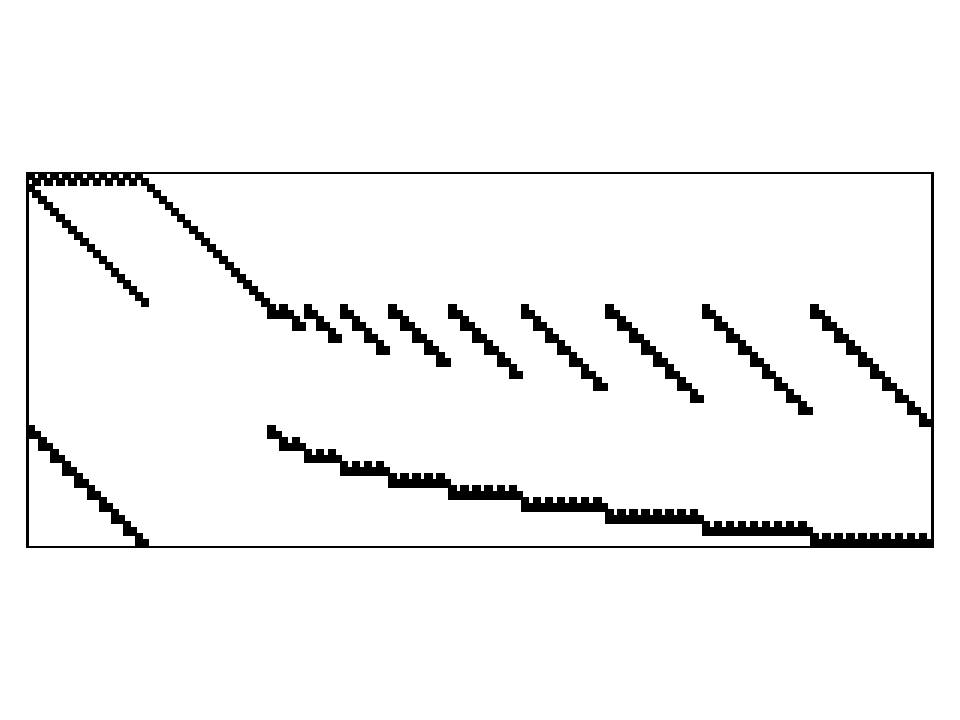
\includegraphics[width=\linewidth]{SIZES_1}
	\caption{SIZES\_1: Extensive form constraint matrix plot}
	\label{fig:sizes_sparsity}
\end{figure}
%In \siplib, only three instances are available in \smps\ files. 

\subsubsection{\sizes: Mathematical formulation}
Suppose a product is available in a finite number $|N|$ of sizes where 1 is the index of the smallest size and $|N|$ is the index of the largest size. Further, suppose size $i$ is substitutable for size $j$ if $i>j$, i.e., larger-sized items may fulfill demand for smaller sizes. Unlike typical cutting-stock problem, an item cannot be substituted into several pieces. 
Let $p_i$ be the unit production cost for size $i$. Generally $p_i>p_j$ for $i>j$. Let $f$ be the fixed setup cost for producing units of any size and $r$ be the unit penalty cost of meeting demand for size $j$ with a larger size $i$. Let $d_{jt}^s$ be the stochastic demand for size $j$ at time $t$ under scenario $l$. Let $c_t^l$ be the stochastic production capacity at time $t$ under scenario $s$. $\PP(s)$ is the equiprobable probability of occurence for scenario $s$.
We introduce three decision variables. The first-stage integer variable $y_{it}$ is the number of units of sizes $i$ produced at time $t$. Another first-stage variable $z_it$ is a binary variable that denotes whether or not we produce size $i$ item at time $t$ under scenario $l$. The second-stage integer variable $x_{ijt}^s$ denotes the number of units of size $i$ cut to meet demand for smaller size $j$ at time $t$ under scenario $s$. For $x_{ijt}^s$ with $i=j$, we use it to indicate that items of length index $i$ are to be used without cutting at time $t$ under scenario $s$.
Based on the above definitions, \sizes\ can be formulated by the following extensive form.

%\begin{subequations}
%	\begin{align}
%	(\texttt{SIZES})\ \textrm{min}\ &\sum_{t\in T}\sum_{i\in N} p_i y_{it} + \sum_{l\in \mathcal{L}} \PP(l)\sum_{t\in T}\left(\sum_{i\in N} sz_{it}^l+r\sum_{i\in N\backslash\{1\}}\sum_{j=1}^{i-1}x_{ijt}^l\right) \label{sizes:obj}\\
%	\textrm{s.t.}\ &\sum_{i\in N}y_{it}\le c_{t}^l,\quad \forall t\in T,\ \forall l\in \mathcal{L}, \label{sizes:b}\\
%	&\sum_{i=j}^{|N|} x_{ijt}^l \ge d_{jt}^l,\quad\forall j\in N,\ \forall t\in T,\  \forall l\in \mathcal{L},\label{sizes:c}\\
%	&\sum_{t'=1}^{t}\sum_{j=1}^{i}x_{ijt'}^l\le\sum_{t'=1}^{t}y_{it'}, \quad\forall i\in N,\ \forall t\in T,\ \forall l\in \mathcal{L},\label{sizes:d}\\
%	&y_{it}\le c_{t}^l z_{it}^l,\quad\forall i \in N,\ \forall t\in T,\ \forall l\in \mathcal{L},\label{sizes:e}\\
%	&y_{it}\in\mathbb{Z}_+,\quad \forall j\in N,\ \forall t\in T,\label{sizes:f}\\
%	&x_{ijt}^l\in\mathbb{Z}_+,\quad\forall i\in N,\ \forall j\in N,\ \forall t\in T,\ \forall l\in \mathcal{L},\label{sizes:g}\\
%	&z_{it}^l\in\{0,1\},\quad\forall i\in N,\ \forall t\in T,\ \forall l\in \mathcal{L}.\label{sizes:h}
%	\end{align}
%\end{subequations}

\begin{subequations} \label{sizes:formulation}
	\begin{align}
	(\sizes)\ \textrm{min}\ &\sum_{t\in T}\sum_{i\in N} \left(fz_{it} + p_i y_{it} \right) + 
	\sum_{s\in \mathcal{S}} \PP(s)\sum_{t\in T}\sum_{i\in N\backslash\{1\}}\sum_{j=1}^{i-1}rx_{ijt}^s \label{sizes:obj}\\
	\textrm{s.t.}\ &\sum_{i\in N}y_{it}\le c_{t},\quad \forall t\in T, \label{sizes:b}\\
	&y_{it}\le c_{t} z_{it},\quad\forall i \in N,\ \forall t\in T,\label{sizes:c}\\
	&\sum_{t'=1}^{t}\sum_{i=j}^{|N|} x_{ijt'}^s \ge d_{jt}^s,\quad\forall j\in N,\ \forall t\in T,\  \forall s\in \mathcal{S},\label{sizes:d}\\
	&\sum_{t'=1}^{t}\sum_{j=1}^{i}x_{ijt'}^s\le\sum_{t'=1}^{t}y_{it'}, \quad\forall i\in N,\ \forall t\in T,\ \forall s\in \mathcal{S},\label{sizes:e}\\
	&y_{it}\in\mathbb{Z}_+,\quad \forall j\in N,\ \forall t\in T,\label{sizes:f}\\
	&z_{it}\in\{0,1\},\quad\forall i\in N,\ \forall t\in T,\label{sizes:g}\\
	%&x_{ijt}^s\in\mathbb{Z}_+,\quad\forall i\in N,\ \forall j\in N,\ \forall t\in T,\ \forall s\in \mathcal{S}.\label{sizes:h} \\
	&x_{ijt}^s\in\mathbb{Z}_+,\quad\forall (i,j:i\ge j)\in N\times N,\ \forall t\in T,\ \forall s\in \mathcal{S}.\label{sizes:h}
	\end{align}
\end{subequations}

The first sum of the objective function (\ref{sizes:obj}) is the costs for producing items for all time periods (fixed + variable costs). The second term corresponds to the expectation of the penalty costs for substituting items. Constraint (\ref{sizes:b}) ensures the production for each period cannot exceed the capacity under all scenarios. Constraint (\ref{sizes:c}) is the logical constraint for the cost expression. (\ref{sizes:d}) guarantees the demand for each item can be met for all time periods and for all scenarios. Notice that constraint (\ref{sizes:d}) means the demand can be met by the items that are produced in the previous periods as well. Constraint (\ref{sizes:e}) enforces the supply limit. Constraints (\ref{sizes:f})-(\ref{sizes:h}) are binary or integer restrictions of the decision variables.

\begin{table}[H]
	\caption{Notations for \sizes}
	\label{sizes:notation}
	\resizebox{\textwidth}{!}
	{
		\begin{tabular}{ll}
			\toprule
			\multicolumn{2}{l}{\textbf{Index sets}} \\
			$N$ & \textrm{index set of items ($i,j\in N$)} \\ 
			$T$ & \textrm{index set of time periods ($t\in T$)} \\ 
			$\mathcal{S}$ & \textrm{index set of scenarios ($s\in\mathcal{S}$)}\\ \midrule
			\multicolumn{2}{l}{\textbf{Parameters}} \\
			$p_{i}$ & unit production cost for item $i$\\
			$f$	& fixed setup cost for producing any item\\
			$r$ & unit cutting cost\\ 
			$c_{t}$ & production capacity at time $t$\\
			$d_{it}^s$ &	demand for item $i$ at time $t$ under scenario $s$\\
			$\PP(s)$ & the probability of occurence of scenario $s$\\ \midrule
			\multicolumn{2}{l}{\textbf{Decision variables}} \\
			$y_{it}$ (1st-stage)  & number of units of size $i$ produced at time $t$ \\
			$z_{it}$ (1st-stage)& 1 if we produce size $i$ at time $t$, 0 otherwise\\
			$x_{ijt}^s$ (2nd-stage) & number of units of size $i$ cut to meet demand for smaller size $j$ at time $t$ under scenario $s$\\ 
			\bottomrule
		\end{tabular}
	}
\end{table} 

%\begin{table}[H]
%	\caption{Notations for \texttt{SIZES}}
%	\label{sizes:notation}
%	\resizebox{\textwidth}{!}
%	{
%		\begin{tabular}{ll}
%			\toprule
%			\multicolumn{2}{l}{\textbf{Index sets}} \\
%			$N$ & \textrm{index set of items ($i,j\in N$)} \\ 
%			$T$ & \textrm{index set of time periods ($t\in T$)} \\ 
%			$\mathcal{L}$ & \textrm{index set of scenarios ($l\in\mathcal{L}$)}\\ \midrule
%			\multicolumn{2}{l}{\textbf{Parameters}} \\
%			$d_{it}^l$ &	demand for item $i$ at time $t$ under scenario $l$\\
%			$p_{i}$ & unit production cost for item $i$\\
%			$s$	& setup cost for producing any item\\
%			$r$ & unit cutting cost\\ 
%			$c_{t}^l$ & production capacity at time $t$ under scenario $l$\\
%			$\PP(l)$ & the probability of occurence of scenario $l$\\ \midrule
%			\multicolumn{2}{l}{\textbf{Decision variables}} \\
%			$y_{it}$ ($1^{\textrm{st}}$ stage)  & number of units of size $i$ produced at time $t$ \\
%			$x_{ijt}^l$ ($2^{\textrm{nd}}$ stage) & number of units of size $i$ cut to meet demand for smaller size $j$ at time $t$ under scenario $l$\\ 
%			$z_{it}^l$ ($2^{\textrm{nd}}$ stage)& 1 if we produce size $i$ at time $t$ under scenario $l$, 0 otherwise\\
%			\bottomrule
%		\end{tabular}
%	}
%\end{table} 

\subsubsection{\sizes: Data generation}
Instances of \sizes\ are generated based on the one-period data given in Table \ref{sizes:data}. Note that although the table includes sleeve length data, we do not use this information for \sizes\ since this is not a typical cutting stock problem. Following \cite{journal:JSW1999}, we set the stochastic parameter $c_t^s=200,000$ to be deterministic for all $t\in T$ and $s\in\mathcal{S}$, hence only the demand parameter ($d_i^s$) is stochastic throughout the scenarios. The stochastic demand data is generated based on Table \ref{sizes:data}. First, we decide the number of scenarios to be generated by $|\mathcal{S}|$. Then, the demand data is specified by a vector of multipliers: one multiplier for each scenario that is multiplied times the demand vector from Table \ref{sizes:data}. For example, if $|\mathcal{S}|=3$, the instance is defined by $(0.7,1,1.3)$. Or if $|\mathcal{S}|=5$, the instance is defined by $(0.6,0.8,1,1.2,1.4)$. Since \siplib\ provides instances with $|\mathcal{S}|\le 20$, we recommend the users to use \siplibtwo\ to only generate instances with $|\mathcal{S}| \ge 20$. In \siplibtwo\, the multiplier vector is defined by the equally split set of subintervals between $[0.5,1.5]$, e.g., when $|\mathcal{S}|=20$, the multiplier vector is $(0.5,0.55,0.6,\ldots,1.4,1.45,1.5)$. With larger value of $|\mathcal{S}|$, we will have vector with finer granularity. To generate more random instances, the demand vector is multiplied by a continuous random number $U$ that is uniformly distributed in $(0.5,1.5)$. After that, the instance is named by SIZES\_$|\mathcal{S}|$.

\begin{table}[]
	\centering
	\caption{Base data for \sizes\ scenarios \cite{journal:JSW1999}}
	\label{sizes:data}
	\begin{tabular}{cccc}
		\hline
		$i$  & sleeve length & unit production cost ($p_i$) & demand ($d_i$) \\ \hline
		1  & 25            & 0.748                & 2500   \\
		2  & 30            & 0.7584               & 7500   \\
		3  & 35            & 0.7688               & 12500  \\
		4  & 40            & 0.7792               & 10000  \\
		5  & 45            & 0.7896               & 35000  \\
		6  & 50            & 0.8                  & 25000  \\
		7  & 55            & 0.8014               & 15000  \\
		8  & 60            & 0.8208               & 12500  \\
		9  & 65            & 0.8312               & 12500  \\
		10 & 70            & 0.8416               & 5000   \\ \hline
		\multicolumn{4}{c}{unit cutting cost ($u$): \$0.008}     \\
		\multicolumn{4}{c}{setup cost ($f$): \$453}              \\ 
		\multicolumn{4}{c}{production capacity ($c_t$): 200,000} \\ \hline
	\end{tabular}
\end{table}

\subsection{\smkp: Stochastic multiple knapsack problem} \label{SMKP}
\smkp\ is a class of stochastic multiple binary knapsack problems. Unlike typical knapsack problems where the objective is to maximize total profits under the restriction of the weight capacity of each knapsack, \smkp\ is to minimize total weights while satisfying a certain required profit for each knapsack. 

\siplib\ provides 30 instances of \smkp\ in total. The first-stage problems contain 240 binary variables and 50 knapsack constraints. The second-stage problems have 120 binary variables and 5 knapsack constraints. Each instance has 20 scenarios. 
We mainly refer to \cite{journal:AAD2014}.% for writing \texttt{Julia} script for \siplibtwo\ and explain the model throughout the following subsections.

Fig. \ref{fig:smkp_sparsity} shows the sparsity pattern presents in extensive form \smkp\ (single scenario).
\begin{figure}[H]
	\centering
	
\includegraphics[width=\linewidth]{SMKP_50_1}
	\caption{SMKP\_50\_1: Extensive form constraint matrix plot}
	\label{fig:smkp_sparsity}
\end{figure}

\subsubsection{\smkp: Mathematical formulation}
We have three types of items $x$, $z$, and $y$ where the first two types are of the first-stage and the last one is of the second-stage with stochastic scenarios. For each type, we have $|I|$ number of items where $I$ is the index set of the items. Hence, we define the binary variables $x_i$, $z_i$, and $y_i^s$ which are equal to 1 if the $i^{\mathrm{th}}$ item is decided to be included ($s$ denotes scenario so only appears in $y$-type variables). We consider two types of knapsacks: one associated with $x$-type and $z$-type items (say \texttt{xz}-knapsack) and the other one with $x$-type and $y$-type items (say \texttt{xy}-knapsack). \texttt{xz}-knapsacks are indexed by $j\in J$ and \texttt{xy}-knapsacks are indexed by $k\in K$.  Each knapsack has its own minimum level of profit that should be satisfied by the items of the associated types, e.g., the profit of the $j^{\mathrm{th}}$ \texttt{xz}-type knapsack is calculated based on the inclusion or exclusion of $x$-type and $z$-type items and should satisfy a certain requirement $b_j$. Bear in mind that the inclusion or exclusion of a certain item $i$ affects all the associated knapsacks.
 
Each parameter $c_i$, $d_i$, and $q_i^s$ denotes the gain of weight when including items of type $x$, $z$, and $y$, respectively. Here, $c_i$ and $d_i$ are deterministic and $q_i^s$ is stochastic. Parameters $a_{ji}$, $e_{ji}$, $t_{ki}$, and $w_{ki}$ are all deterministic and denote the profits for including items in the knapsacks. The RHS parameters $b_j$ and $h_k$ are the minimum levels of profit requirements for \texttt{xz}-knapsacks and \texttt{xy}-knapsacks, respectively.

The extensive form of \smkp\ is as follows and the notations used are summarized in Table \ref{smkp:notation}.
\begin{subequations} \label{smkp:formulation}
	\begin{align}
	(\smkp)\ \textrm{min}\ &\sum_{i \in I}\left(c_i x_i + d_i z_i\right) + \sum_{s\in\mathcal{S}}\PP(s)\sum_{i\in I}q_i^s y_i^s \label{smkp:obj}\\
	\textrm{s.t.}\ &  \sum_{i\in I}a_{ji}x_{i} + \sum_{i \in I}e_{ji}z_i\ge b_j,\quad\forall j\in J, \label{smkp:b}\\
	&  \sum_{i\in I} t_{ki}x_i + \sum_{i\in I}w_{ki} y_i^s\ge h_k,\quad\forall k\in K,\ \forall s\in\mathcal{S}, \label{smkp:c}\\
	&  x_i\in\{0,1\},\quad\forall i\in I, \label{smkp:d}\\
	&  z_i\in\{0,1\},\quad\forall i\in I, \label{smkp:e}\\
	&  y_i^s\in\{0,1\},\quad\forall i\in I,\ \forall s\in \mathcal{S}. \label{smkp:f}
	\end{align}
\end{subequations}

The objective (\ref{smkp:obj}) is to minimize the expected value of the total weights. Constraint (\ref{smkp:b}) ensures the minimum levels of profit requirements for all \texttt{xz}-knapsacks are satisfied. Constraint (\ref{smkp:c}) guarantees the minimum levels of profit requirements are satisfied for all \texttt{xy}-knapsacks under every scenario. Constraints (\ref{smkp:d})-(\ref{smkp:f}) are binary restriction of the decision variables.

\begin{table}[H]
	\caption{Notations for \smkp}
	\label{smkp:notation}
	\resizebox{\textwidth}{!}
	{
		\begin{tabular}{ll}
			\toprule
			\multicolumn{2}{l}{\textbf{Index sets:}} \\
			$I$ &  index set of items for each type ($i\in I$)\\ 
			$J$ &  index set of \texttt{xz}-knapsacks ($j \in J$)\\ 
			$K$ &  index set of \texttt{xy}-knapsacks ($k \in K$)\\
			$\mathcal{S}$ & index set of scenarios ($s\in \mathcal{S}$)\\ \midrule
			\multicolumn{2}{l}{\textbf{Parameters:}} \\
			$c_{i}$ 	& weight of the $i^{\mathrm{th}}$ $x$-type item 		\\ 
			$d_{i}$ 	& weight of the $i^{\mathrm{th}}$ $z$-type item  		\\ 
			$q_{i}^{s}$ & weight of the $i^{\mathrm{th}}$ $y$-type item under scenario $s$ 		\\ 
			$a_{ji}$	& profit of the $j^{\mathrm{th}}$ \texttt{xz}-knapsack for including $i^{\mathrm{th}}$ $x$-type item		\\
			$e_{ji}$	& profit of the $j^{\mathrm{th}}$ \texttt{xz}-knapsack for including $i^{\mathrm{th}}$ $z$-type item		\\
			$t_{ki}$	& profit of the $k^{\mathrm{th}}$ \texttt{xy}-knapsack for including $i^{\mathrm{th}}$ $x$-type item	\\
			$w_{ki}$	& profit of the $k^{\mathrm{th}}$ \texttt{xy}-knapsack for including $i^{\mathrm{th}}$ $y$-type item		\\
			$b_j$		& minimum required profit for the $j^{\mathrm{th}}$ \texttt{xz}-knapsack		\\
			$h_k$		& minimum required profit for the $k^{\mathrm{th}}$ \texttt{xy}-knapsack		\\
			$\PP(s)$ 	& \textrm{the probability of occurence of scenario $s$} \\ \midrule
			\multicolumn{2}{l}{\textbf{Decision variables:}} \\
			$x_{i}$ (1st-stage) & 1 if the $i^{\mathrm{th}}$ $x$-type item is decided to be included, 0 otherwise \\ 
			$z_{i}$ (1st-stage) & 1 if the $i^{\mathrm{th}}$ $z$-type item is decided to be included, 0 otherwise \\ 
			$y_{i}^s$ (2nd-stage)& 1 if the $i^{\mathrm{th}}$ $y$-type item is decided to be included under scenario $s$, 0 otherwise  \\
			\bottomrule
		\end{tabular}
	}
\end{table} 

\subsubsection{\smkp: Data generation}
There are two factors that define the instance of \smkp: $|I|$ and $|\mathcal{S}|$. The sizes for another sets are fixed by $|J|=50$ and $|K|=5$ following \cite{journal:AAD2014}. Once we decide the factors $|I|$ and $|\mathcal{S}|$, each instance is named by SMKP\_$|I|$\_$|\mathcal{S}|$. Again directly following \cite{journal:AAD2014}, we randomly generate the parameters. Let $U$ be a discrete uniform random variable: $U\sim Unif[1,100]$. Then, the parameters are generated as follows:
\begin{align*}
c_i		&=	U,\quad\forall i\in I, \\
d_i		&=	U,\quad\forall i\in I, \\
q_i^s	&= 	U,\quad\forall i\in I,\ \forall s\in\mathcal{S},\\
a_{ji}	&=	U,\quad\forall j\in J,\ \forall i\in I, \\
e_{ji}	&=	U,\quad\forall j\in J,\ \forall i\in I, \\
t_{ki}	&=	U,\quad\forall k\in K,\ \forall i\in I, \\
w_{ki}	&=	U,\quad\forall k\in K,\ \forall i\in I,  \\
b_j		&=	\frac{3}{4}\sum_{i\in I}\left(a_{ji}+e_{ji}\right),\quad\forall j\in J, \\
h_k		&=	\frac{3}{4}\sum_{i\in I}\left(t_{ji}+w_{ji}\right),\quad\forall k\in K. 
\end{align*}

\subsection{\sslp: Stochastic server location problem} \label{SSLP}
\sslp\ is a class of problem that finds the optimal location of servers and the optimal allocation of clients to servers which maximizes the expected net income under uncertain presents of clients. \sslp\ finds applications in a variety of domains such as network design for electric power, internet services, telecommunications, and water distribution. \siplib\ provides 12 instances with varying number of clients, server locations, and scenarios in \smps\ format. The largest instance includes 10 server locations, 50 clients, and 2,000 scenarios which corresponds to 120,001 constraints, 1,000,010 binary variables, and 20,000 continuous variables. We refer to \cite{journal:NS2005} for mathematical formulation and data generation forthcoming through the following subsections.

Fig. \ref{fig:sslp_sparsity} shows the sparsity pattern presents in extensive form \sslp\ (single scenario).
\begin{figure}[]
	\centering
	
\includegraphics[width=\linewidth]{SSLP_4_4_1}
	\caption{SSLP\_4\_4\_1: Extensive form constraint matrix plot}
	\label{fig:sslp_sparsity}
\end{figure}

\subsubsection{\sslp: Mathematical formulation}
Let $I$, $J$, $Z$, and $\mathcal{S}$ be index sets for the clients, servers, zones, and scenarios. For $i\in I$, $j\in J$, $z\in Z$, and $s\in\mathcal{S}$, we define the notations in Table \ref{sslp:notation}.

Suppose that we place a server at location $j$. Then, the allocation costs $c_j$ and the server will provide capacity to serve up to $u$ amount of resource to clients. The revenue earned by serving client $i$ from location $j$ is denoted by $q_{ij}$. We have also a shortage cost (penalty) $q_{0j}$ for each unit of demand that remains unserved among the clients assigned to server $j$. If client $i$ is served by a server at location $j$, it uses $d_{ij}$ units of resource from the server. We allow only one server to be installed at each location and each client can only be served by one server. There is a requirement that a minimum number of servers to be located in a zone $z$, and is denoted by $w_z$. 

The first-stage binary variables $x_j$ decide whether or not a server is located at location $j$. The second-stage binary variables $y_{ij}^s$ are referred to as recourse decision under scenario $s$ and associated with the decision on serving client $i$ by server $j$. The variables $y_{ij}^s$ will be implemented in the future, when scenario $s$ is finally observed.

Based on the above, the extensive form of \sslp\ can be stated as follows:
\begin{subequations} \label{sslp:formulation}
	\begin{align}
	(\sslp)\ \textrm{min}\ &	\sum_{j\in J}c_j x_j - \sum_{s\in\mathcal{S}}\PP(s)\left(\sum_{i\in I}\sum_{j\in J}q_{ij}^s y_{ij}^s - \sum_{j\in J}q_{0j}^s y_{0j}^s \right) \label{sslp:obj} \\ 
	\textrm{s.t.}\ &\sum_{j\in J}x_j\le v,\label{sslp:b}\\ 
	&\sum_{j\in J_z}x_j\ge w_z,\quad\forall z\in Z,\label{sslp:c}\\
	&\sum_{i\in I}d_{ij}y_{ij}^s - y_{0j}^s\le ux_j,\quad\forall j\in J,\ \forall s\in\mathcal{S}, \label{sslp:d} \\
	&\sum_{j\in J}y_{ij}^s=h_i^s,\quad\forall i\in I,\ \forall s\in \mathcal{S}, \label{sslp:e}\\
	&x_j\in\{0,1\},\quad\forall j\in J,\label{sslp:f}\\
	&y_{ij}^s\in\{0,1\},\quad\forall i\in I,\ j\in J,\ s\in\mathcal{S}, \label{sslp:g}\\
	&y_{0j}^s\ge 0,\quad\forall j\in J,\ \forall s\in\mathcal{S} \label{sslp:h}.
	\end{align}
\end{subequations}
The objective function (\ref{sslp:obj}) is to maximize total expected revenue of locating servers and serving customers by the servers. Constraint (\ref{sslp:b}) satisfies the requirement that only up to a total of $v$ available servers can be installed. The zonal requirements that specify how many servers are needed in each zone are given by constraint (\ref{sslp:c}). Constraint (\ref{sslp:d}) ensures that a server located at site $j$ can serve only up to its capacity $u$. The variable $y_{0j}^s$ is introduced in the constraint (\ref{sslp:d}) to accomodate any overflows that are not served due to limitations in server capacity. These overflows result in a loss of revenue at a rate of $q_{0j}^s$. The inclusion of an artificial variable may allow a client to be assigned to servers that are not located. However, penalty costs associated with such an assignment may result in such high costs as to preclude it in an optimal solution, unless server capacity is so limited that some clients have to be turned away \cite{journal:NS2005}. Constraint (\ref{sslp:e}) guarantees that each client is served by only one server. Constraint (\ref{sslp:f}) and (\ref{sslp:g}) are binary restrictions on the decision variables. Finally, constraint (\ref{sslp:h}) is the non-negativity requirement on the overflow variables.
\begin{table}[H]
	\caption{Notations for \sslp}
	\label{sslp:notation}
	\resizebox{\textwidth}{!}
	{
		\begin{tabular}{ll}
			\toprule
			\multicolumn{2}{l}{\textbf{Index sets:}} \\
			$J$ 		  & index set of server locations ($j\in J$)\\ 
			$I$ 		  & index set of clients ($i\in I$)  \\ 
			$Z$ 		  & index set of zones ($z\in Z$) \\
			$\mathcal{S}$ & index set of scenarios ($s\in \mathcal{S}$)	\\ \midrule
			\multicolumn{2}{l}{\textbf{Parameters:}} \\
			$c_j$		& cost of locating a server at location $j$	\\
			$q_{ij}^s$	& revenue from client $i$ being served by server at location $j$ under scenario $s$	\\
			$q_{0j}^s$	& rate of revenue loss for overflows that are not served due to limited server capacity under scenario $s$	\\
			$d_{ij}$	& resource demand of client $i$ from server at location $j$	\\
			$u$			& server capacity	\\
			$v$			& upper bound on the total number of servers that can be located	\\
			$w_z$		& minimum number of servers to be located in zone $z$	\\
			$J_z$		& subset of server locations that belong to zone $z$	\\
			$h_i^s$		& 1 if client $i$ is present under scenario $s$, 0 otherwise	\\
			$\PP(s)$ 	& probability of occurence for scenario $s$\\ \midrule
			\multicolumn{2}{l}{\textbf{Decision variables:}} \\
			$x_j$ (1st-stage)  	 & 1 if a server is located at site $j$, 0 otherwise \\
			$y_{ij}^s$ (2nd-stage) & 1 if client $i$ is served by a server at location $j$ under scenario $s$, 0 otherwise\\
			$y_{0j}^s$ (2nd-stage) & non-negative amount of overflows that are not served due to limitations in server $j$'s capacity	\\
			\bottomrule
		\end{tabular}
	}
\end{table} 

\subsubsection{\sslp: Data generation}
For each instance of \sslp\, we determine the number of potential server locations $|J|$, the number of clients $|I|$, and the number of scenarios $|\mathcal{S}|$. Then, the instance is named by SSLP\_$|J|$\_$|I|$\_$|\mathcal{S}|$. The client-server revenue are set to be 1 per unit of client demand. Some of deterministic parameters are randomly generated from the discrete uniform distribution while scenario data are generated from the Bernoulli distribution. In summary, the parameters are generated as follows:
\begin{align*}
c_j	&=Unif[40,80],\quad\forall j\in J,\\
d_{ij}	&= Unif[0,25],\quad\forall i\in I,\ \forall j\in J,\\
h_i^s	&= Bernoulli(0.5),\quad\forall i\in I,\ \forall s\in \mathcal{S},\\
q_{ij}^s	&= d_{ij},\quad\forall i\in I,\ \forall j\in J,\ \forall s\in\mathcal{S},\\
q_{0j}^s	&=	1000,\quad\forall j\in J,\ \forall s\in\mathcal{S},\\
v 		&= |J|	\\
u	&= \frac{3}{2}\times\frac{\sum_{i\in I}\sum_{j\in J}d_{ij}}{|J|} 
\end{align*}
Note that the zonal data is omitted due to the lack of available information. Hence, constraint (\ref{sslp:c}) does not appear in \siplibtwo\ instances. Note also that constraint (\ref{sslp:b}) is redundant since we set $v=|J|$. We include this redundant constraint to follow the former \siplib\ implementation although it seems like a bug.

\subsection{\suc: Stochastic unit commitment problem} \label{SUC}
The unit commitment (UC) problem is a production cost model (PCM) that plans power system operations over an extended time horizon. \suc\ is a stochastic version of UC for studying the impact of incorporating highly uncertain power generation of large-scale wind turbines with transmission constraints and system component failures. We refer to \cite{journal:PO2013} for mathematical models. For model parameters, we use Western Electricity Coordinating Council data set (WECC \cite{web:wecc}) interconnected with California ISO Open Access Same-Time Information System (CAISO) as in the reference. 

Fig. \ref{fig:suc_sparsity} shows the sparsity pattern presents in extensive form \suc\ (single scenario).
\begin{figure}[H]
	\centering
	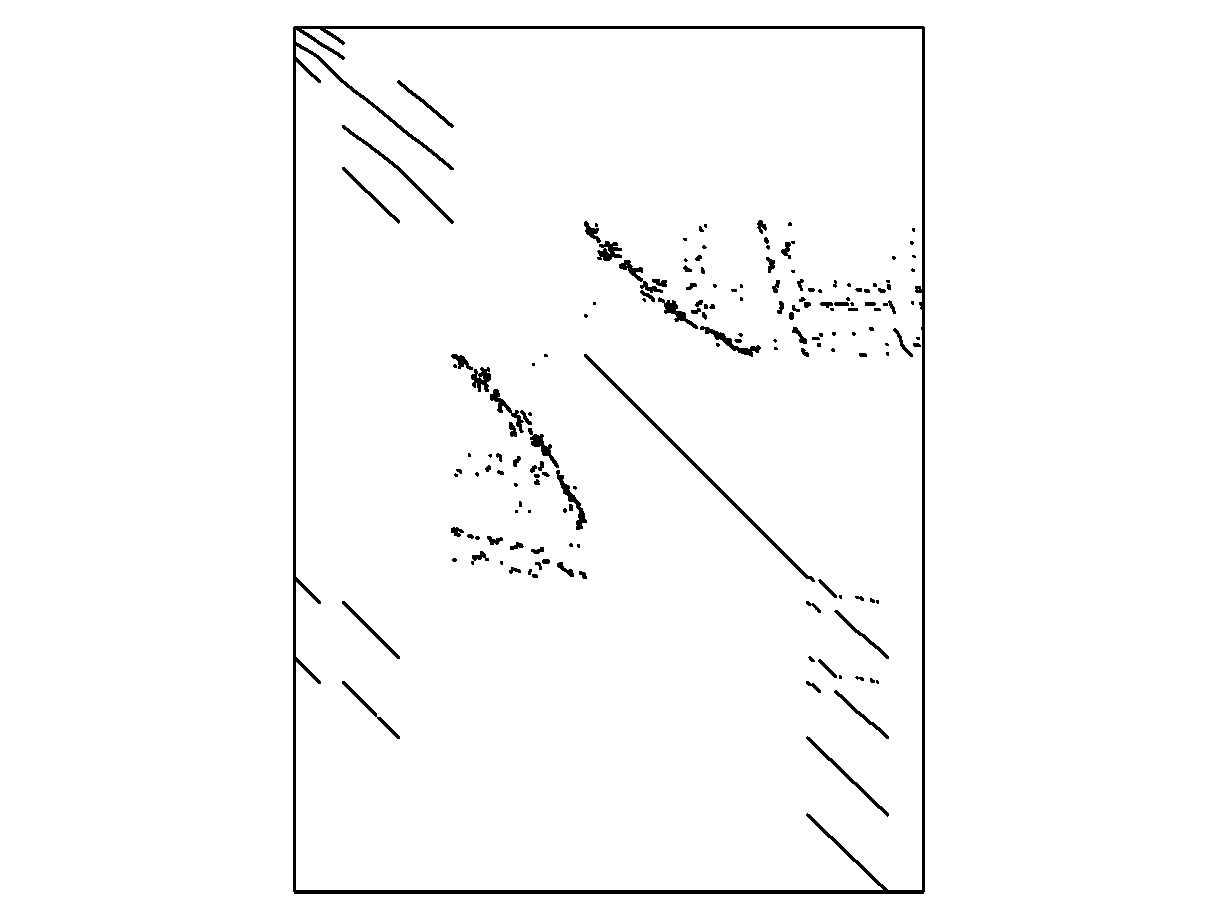
\includegraphics[width=\linewidth]{SUC_FallWD_1}
	\caption{SUC\_FallWD\_1: Extensive form constraint matrix plot}
	\label{fig:suc_sparsity}
\end{figure}

\subsubsection{\texttt{SUC}: Mathematical formulation}
In \suc, we make commitment decision on slow generators in the first stage. In the second stage, the commitment decisions of fast generators, wind generators, and non-wind renewable generators, shedding decisions of loads, and import decisions from other points are determined. In addition, phase angle for each transmission line is decided in the second stage. In \suc, we also consider ramping constraints, transmission line capacity constraints, phase angle constraints, and minimum up/down time constraints. We assume the piecewise linear convex cost function for the power generation.

Using the notation in Table \ref{SUC:notation}, the extensive form of \suc\ can be stated as in the following model \ref{SUC:formulation}.
\begin{subequations} \label{SUC:formulation}
	\begin{align}
	(\suc)\ \textrm{min}\ &\sum_{g\in G_s}\sum_{t \in T}\left(K_g w_{gt}+S_g z_{gt}\right) \nonumber \\	
	&+ \sum_{s\in\mathcal{S}}\PP(s)\sum_{t\in T} 
	\Bigg[	 \sum_{g\in G_f} \left(K_g u_{gts}+S_g v_{gts}\right) + \sum_{g\in G}C_g p_{gts} + \sum_{\lambda\in \mathcal{L}} C^{\mathcal{L}}x_{\lambda ts}^{\mathcal{L}} \nonumber \\&\qquad\qquad\qquad\qquad\qquad\quad  + \sum_{\iota\in \mathcal{I}} C^{\mathcal{I}}x_{\iota ts}^{\mathcal{I}} + \sum_{\rho\in \mathcal{R}} C^{\mathcal{R}}x_{\rho ts}^{\mathcal{R}} + \sum_{\omega\in \mathcal{W}} C^{\mathcal{W}}x_{\omega ts}^{\mathcal{W}} \Bigg]
	\label{SUC:obj}\\
	\textrm{s.t.}\ &  \textrm{(First-stage constraints)} \nonumber\\
	&\sum_{q=t-UT_g+1}^t z_{gq}\le w_{qt},\quad\forall g\in G_s,\ \forall t\ge UT_g,	\label{SUC:b}\\
	&\sum_{q=t+1}^{t+DT_g} z_{gq}\le 1-w_{gt},\quad\forall g\in G_s,\ \forall t\le |T|-DT_g,\label{SUC:c}\\
	&z_{gt}\ge w_{gt}-w_{g,t-1},\quad\forall g\in G_s,\ \forall t\in T,\label{SUC:d}\\
	&  \textrm{(Second-stage constraints)} \nonumber\\
	&  \sum_{q=t-UT_g+1}^t v_{gqs}\le u_{qts},\quad\forall g\in G_f,\ \forall t\ge UT_g,\ \forall s\in\mathcal{S},\label{SUC:e}\\
	&\sum_{q=t+1}^{t+DT_g} v_{gqs}\le 1-u_{gts},\quad\forall g\in G_f,\ \forall t\le |T|-DT_g,\ \forall s\in\mathcal{S},\label{SUC:f}\\
	&v_{gts}\ge u_{gts}-u_{g,t-1,s},\quad\forall g\in G_f,\ \forall t\in T,\ \forall s\in\mathcal{S},\label{SUC:g}\\
	&\sum_{l\in L_n^-}f_{lts}+\sum_{g\in G_n} p_{gts}+\sum_{\lambda\in IG_n^\mathcal{L}}x_{\lambda ts}^\mathcal{L} +\sum_{\omega\in IG_n^\mathcal{W}} IC_{\omega ts}^\mathcal{W} \nonumber \\ 
	&= D_{nt}+\sum_{l\in L_n^+}f_{lts}+\sum_{\iota\in IG_n^\mathcal{I}}x_{\iota ts}^\mathcal{I} + \sum_{\rho\in IG_n^\mathcal{R}} x_{\rho ts}^\mathcal{R} +\sum_{\omega\in IG_n^\mathcal{W}} x_{\omega ts}^\mathcal{W}, \nonumber \\
	&\qquad\qquad\qquad\qquad\qquad\qquad\qquad\qquad\qquad\forall n\in N,\ \forall t\in T,\ \forall s\in\mathcal{S},\label{SUC:h}\\
	&f_{lts}=B_l\left(  \theta_{n_1 ts}-\theta_{n_2 ts}  \right),\quad\forall l\equiv (n_1, n_2)\in L,\ t\in T, s\in\mathcal{S},\label{SUC:i}\\
	&P_g^- w_{gt} \le p_{gts} \le P_g^+ w_{gt},\quad\forall g\in G_s,\ \forall t\in T\cup\{0\},\ \forall s\in\mathcal{S},\label{SUC:j}\\
	&P_g^- u_{gts} \le p_{gts} \le P_g^+ u_{gts},\quad\forall g\in G_f,\ \forall t\in T\cup\{0\},\ \forall s\in\mathcal{S},\label{SUC:k}\\
	&-R_g^- \le p_{gts}-p_{g,t-1,s} \le R_g^+ ,\quad\forall g\in G,\ \forall t\in T,\ \forall s\in\mathcal{S},\label{SUC:l}\\
	&  \textrm{(First-stage variable bounds)} \nonumber\\
	&w_{gt}\in\{0,1\},\quad\forall g\in G_s,\ \forall t\in T\cup\{0\},\label{SUC:m}\\
	& 0\le z_{gt}\le 1,\quad\forall g\in G_s,\ \forall t\in T,\label{SUC:n}\\
	&  \textrm{(Second-stage variable bounds)} \nonumber\\
	&u_{gts}\in\{0,1\},\quad\forall g\in G_f,\ \forall t\in T\cup\{0\},\ \forall s\in\mathcal{S},\label{SUC:o}\\
	&0\le v_{gts}\le 1,\quad\forall g\in G_f,\ \forall t\in T,\ \forall s\in\mathcal{S},\label{SUC:p}\\
	&-360\le\theta_{nts}\le 360,\quad\forall n\in N,\ \forall t\in T,\ \forall s\in\mathcal{S},\label{SUC:q}\\
	&-TC_l\le f_{lts}\le TC_l,\quad\forall l\in L,\ \forall t\in T,\ \forall s\in\mathcal{S},\label{SUC:r}\\
	&p_{gts}\ge 0,\quad\forall g\in G,\ \forall t\in T\cup\{0\},\ \forall s\in\mathcal{S},\label{SUC:s}\\
	&0\le x_{\lambda ts}^\mathcal{L}\le IC_{\lambda t}^\mathcal{L},\quad\forall \lambda\in \mathcal{L},\ \forall t\in T,\ \forall s\in\mathcal{S},\label{SUC:t}\\
	&0\le x_{\iota ts}^\mathcal{I}\le IC_{\iota t}^\mathcal{I},\quad\forall \iota \in \mathcal{I},\ \forall t\in T,\ \forall s\in\mathcal{S},\label{SUC:u}\\
	&0\le x_{\rho ts}^\mathcal{R} \le IC_{\rho t}^\mathcal{R},\quad\forall \rho\in\mathcal{R},\ \forall t\in T,\ \forall s\in\mathcal{S},\label{SUC:v}\\
	&0\le x_{\omega ts}^\mathcal{W}\le IC_{\omega t}^W,\quad\forall \omega\in\mathcal{W},\ \forall t\in T,\ \forall s\in\mathcal{S}.\label{SUC:w}
	\end{align}	
\end{subequations}

The objective function (\ref{SUC:obj}) is to minimize expected operating costs. Constraints (\ref{SUC:b})-(\ref{SUC:d}) are for the first-stage so constraints for the slow generators. Constraint (\ref{SUC:b}) and (\ref{SUC:c}) represent the minimum up/down time of the slow generators. The transition rule for slow generator start-up variables is imposed by constraint (\ref{SUC:d}).  Constraints (\ref{SUC:e})-(\ref{SUC:g}) are stochastic version of the constraints (\ref{SUC:b})-(\ref{SUC:d}) so represent the minimum up/down time and the transition rule of the fast generators. Constraint (\ref{SUC:h}) requires balancing the amount of power that flows in and out of each bus. Constraint (\ref{SUC:i}) represents a linearized, lossless model of the power flow equations (Kirchhoff's law) according to which the power flow on a line $l$ is proportional to the phase angle difference between the two end buses of the line. Constraints (\ref{SUC:j}) and (\ref{SUC:k}) restrict minimum/maximum capacity limits for both slow and fast generators. Constraint (\ref{SUC:l}) represents ramping restriction on the rate of change of generator output. Constraints (\ref{SUC:m})-(\ref{SUC:w}) define the types and bounds for decision variables.
\begin{table}[H]
	\centering
	\caption{Notations for \suc}
	\label{SUC:notation}
	\resizebox{\textwidth}{!}
	{
		\begin{tabular}{ll}
			\toprule
			\multicolumn{2}{l}{\textbf{Index sets:}} \\
			$\mathcal{S}$ & index set of scenarios ($s\in\mathcal{S}$) 		\\ 		
			$N$ & index set of all buses ($n\in N$)\\
			$T$ & index set of all time periods ($t\in T$)\\
			$L$ & index set of all transmission lines ($l\in L$) \\
			$\mathcal{L}$ & index set of all loads ($\lambda \in \mathcal{L}$)\\
			$\mathcal{I}$ & index set of all import points ($\iota\in \mathcal{I}$)\\
			$\mathcal{R}$ & index set of all non-wind renewable generators ($\rho\in \mathcal{R}$)\\
			$\mathcal{W}$ & index set of all wind generators ($\omega\in \mathcal{W}$)\\
			$G$ & index set of all generators ($g\in G$)\\
			$G_s$ & index set of slow generators ($g\in G_s$)\\
			$G_f$ & index set of fast generators ($g\in G_f$)\\
			\multicolumn{2}{l}{\textbf{(mapping sets)}} \\
			$G_n$ & index set of generators that are located in bus $n$ ($g\in G_n$)\\
			$IG_n^\mathcal{L}$ & index set of loads that bus $n$ can supply ($\lambda\in IG_n^\mathcal{L}$)\\
			$IG_n^\mathcal{I}$ & index set of import points that can supply bus $n$ ($\iota\in IG_n^\mathcal{I}$) \\
			$IG_n^\mathcal{R}$ & index set of non-wind renewable generators that can supply bus $n$ ($\rho\in IG_n^\mathcal{R}$) \\
			$IG_n^\mathcal{W}$ & index set of wind generators that can supply bus $n$ ($\omega\in IG_n^\mathcal{W}$)\\
			$L_n^{+}$ & index set of outgoing transmission lines from bus $n$ ($l\in L_n^+$)\\
			$L_n^{-}$ & index set of incoming transmission lines to bus $n$ ($l\in L_n^-$)\\ \midrule
			\multicolumn{2}{l}{\textbf{Parameters:}} \\
			$\PP(s)$	&probability of occurence for scenario $s$\\
			\multicolumn{2}{l}{\textbf{(cost)}} \\
			$K_g$ & fixed commitment cost of generator $g$ \\
			$S_g$ & fixed startup cost of generator $g$\\
			$C_g$ & marginal generation cost of generator $g$	\\
			$C^\mathcal{L}$ & marginal shedding cost of loads in $\mathcal{L}$	\\
			$C^\mathcal{I}$ & marginal spillage cost of import points in $\mathcal{I}$ \\
			$C^\mathcal{R}$ & marginal spillage cost of non-wind  renewable generators in $\mathcal{R}$ \\ 
			$C^\mathcal{W}$ & marginal spillage cost of wind generators in $\mathcal{W}$ \\
			\multicolumn{2}{l}{\textbf{(capacity)}} \\
			$B_{l}$ & susceptance of line $l$ under scenario $s$\\
			$TC_l$ & capacity of transmission line $l$\\
			$P_{g}^+$ & maximum generation capacity of generator $g$\\
			$P_{g}^-$ & minimum generation capacity of generator $g$ \\
			$R_{g}^+$ & ramping up capacity of generator $g$\\
			$R_{g}^-$ & ramping down capacity of generator $g$\\
			$UT_{g}$ & minimum up time of generator $g$\\
			$DT_{g}$ & minimum down time of generator $g$\\
			\multicolumn{2}{l}{\textbf{(supply/demand)}} \\
			$D_{nt}$ & net demand in bus $n$ at time $t$ \\
			$IC_{\lambda t}^\mathcal{L}$ & demand from load $\lambda$\\
			$IC_{\iota t}^\mathcal{I}$ & generation from import point $\iota$\\
			$IC_{\rho t}^\mathcal{R}$ & generation from renewable generator $\rho$\\
			$IC_{\omega ts}^\mathcal{W}$ & generation from wind generator $\omega$ under scenario $s$\\ \midrule
			\multicolumn{2}{l}{\textbf{Decision variables:}} \\
			$w_{gt}$ (1st-stage) 	& (binary) commitment of slow generator $g$ at time $t$\\
			$z_{gt}$ (1st-stage)	&	(continuous) start-up of slow generator $g$ at time $t$\\
			$u_{gts}$ (2nd-stage)	&	(binary) commitment of fast generator $g$ at time $t$ under scenario $s$\\
			$v_{gts}$ (2nd-stage)	&	(continuous) startup of fast generator $g$ at time $t$ under scenario $s$\\
			$\theta_{gts}$ (2nd-stage)	&	(continuous) phase angle of generator $g$ at time $t$ under scenario $s$\\
			$f_{lts}$ (2nd-stage)	&	(continuous) power flow on line $l$ at time $t$ under scenario $s$\\
			$p_{gts}$ (2nd-stage)	&	(continuous) production of generator $g$ at time $t$ under scenario $s$\\
			$x_{\lambda ts}^\mathcal{L}$	(2nd-stage) & (continuous) shedding from load $\lambda$ at time $t$ under scenario $s$	\\
			$x_{\iota ts}^\mathcal{I}$	(2nd-stage) &	(continuous) spillage for import point $\iota$ at time $t$ under scenario $s$\\
			$x_{\rho ts}^\mathcal{R}$ (2nd-stage)	& (continuous) spillage for non-wind renewable generator $\rho$ at time $t$ under scenario $s$  	\\
			$x_{\omega ts}^\mathcal{W}$ (2nd-stage)	& (continuous) spillage for wind generator $\omega$ at time $t$ under scenario $s$ 	\\
			\hline
		\end{tabular}
	}
\end{table}

\subsubsection{\suc: Data generation}
Each \suc\ instance has two user-specifiable parameters: $D$, and $|\mathcal{S}|$. $D$ is the season-day type which is one of FallWD, FallWE, WinterWD, WinterWE, SpringWD, SpringWE, SummerWD, SummerWE, and $|\mathcal{S}|$ is the number of scenarios. Once the two parameters are decided, the instance in named by SUC\_$D$\_$|\mathcal{S}|$. 

For model parameters, we use a reduced model of the CAISO to follow the reference \cite{journal:PO2013}. The model includes a sparse representation of the entire WECC western interconnect outside of California. 
Based on the WECC, set cardinalities in \suc\ are as follows.
\begin{align*}
|N|&=225 \\
|T|&=24 \\
|L|&=375 \\
|\mathcal{L}|&=40\\
|\mathcal{I}|&=5\\
|\mathcal{R}|&=11\\
|\mathcal{W}|&=5\\
|G|&=130\\
|G_s|&=40\\
|G_f|&=90
\end{align*}

The marginal cost parameters for additional sources (load, import, non-wind renewable, wind) are fixed by
\begin{align*}
C^\mathcal{L}&=5000,\\
C^\mathcal{I}&=C^\mathcal{R}=C^\mathcal{W}=0,
\end{align*}
which means the cost of shedding any load $\lambda$ is 5,000 \$/MWh and no penalty cost for spilling the import, non-wind renewable, and wind sources.

The demand data $D_{nt}$ is assumed to be constant over all scenarios and generated based on the load, import, and non-wind renewable source data as follows.
\begin{align*}
D_{nt}=\sum_{n\in N} \sum_{t\in T}\left(  \sum_{\lambda\in IG_n^\mathcal{L}}IC_{\lambda t}^\mathcal{L} - \sum_{\iota\in IG_n^\mathcal{I}}IC_{\iota t}^\mathcal{I} - \sum_{\rho\in IG_n^\mathcal{R}}IC_{\rho t}^\mathcal{R}    \right),\quad\forall n\in N,\ \forall t\in T.
\end{align*}

Unlike other problems where stochastic data is generated while \julia\ script is running, we pre-generate and provide up to 1,000 wind power production profiles for each day type. This data is included in ``\texttt{$\sim$/Siplib/src/problems/SUC/data/WIND}'' folder and used to generate the stochastic parameter $IC_{\omega ts}^\mathcal{W}$. Hence, the number of scenarios that can be considered in an instance is limited to 1,000, which we think is large enough regarding the intrinsic large-scale size of the problem \suc.
\pagebreak

% general sparsity (fully cardinality based)
\section{Block-wise sparsity based on set cardinality} \label{sec:sparsity}
In this section, we provide block-wise size information as well as the sparsity. Block A is only related with the 1st stage, Block W is only related with the 2nd stage, and Block T is related with both stages. For graphical representation, please refer to Figure \ref{fig:stagewise_sparsity}. Based on this information, one can easily derive the sparsity of the coefficient matrix in extensive form as well.
% DCAP
% Please add the following required packages to your document preamble:
% \usepackage{booktabs}
\begin{table}[h]
	\centering
	\caption{\texttt{DCAP}: fully set cardinality based sparsity information}
	\label{table:sparsity_DCAP}
	\begin{tabular}{@{}lcccc@{}}
		\toprule
		\multicolumn{1}{c}{Block} & \#row    & \#col    & \#nonzero           & Sparsity                   \\ \midrule
		A (1st stage)             & $RT$     & $2RT$    & $2RT$               & $\frac{1}{RT}$             \\
		W (2nd stage)             & $(R+N)T$ & $(1+R)T$ & $NRT+(R+1)NT$       & $\frac{1+2R}{T(R+N)(1+R)}$ \\
		T (complicating)          & $(R+N)T$ & $2RT$    & $\frac{1}{2}T(T+1)$ & $\frac{1+T}{4T(R+N)}$      \\ \bottomrule
	\end{tabular}
\end{table}


% DCLP


% MPTSPs
% Please add the following required packages to your document preamble:
% \usepackage{booktabs}
\begin{table}[h]
	\centering
	\caption{\texttt{MPTSPs}: fully set cardinality based sparsity information}
	\label{table:sparsity_MPTSPs}
	\begin{tabular}{@{}lcccc@{}}
		\toprule
		\multicolumn{1}{c}{Block} & \#row    & \#col     & \#nonzero      & Sparsity                \\ \midrule
		A (1st stage)             & $N(N+1)$ & $2N(N-1)$ & $2(3N-2)(N-1)$ & $\frac{3N-2}{(N+1)N^2}$ \\
		W (2nd stage)             & $N(N-1)$ & $KN(N-1)$ & $N(N-1)$       & $\frac{1}{KN(N-1)}$     \\
		T (complicating)          & $N(N-1)$ & $2N(N-1)$ & $3N(N-1)$      & $\frac{3}{2N(N-1)}$     \\ \bottomrule
	\end{tabular}
\end{table}


% SIZES
% Please add the following required packages to your document preamble:
% \usepackage{booktabs}
\begin{table}[h]
	\centering
	\caption{\texttt{SIZES}: fully set cardinality based sparsity information}
	\label{table:sparsity_SIZES}
	\begin{tabular}{@{}lcccc@{}}
		\toprule
		\multicolumn{1}{c}{Block} & \#row    & \#col    & \#nonzero                 & Sparsity             \\ \midrule
		A (1st stage)             & $T(N+1)$ & $2NT$    & $3NT$                     & $\frac{3}{2T(N+1)}$ \\
		W (2nd stage)             & $2NT$    & $N(N+1)$ & $\frac{1}{2}NT(T+1)(N+1)$ & $\frac{T+1}{4N}$    \\
		T (complicating)          & $2NT$    & $2NT$    & $\frac{1}{2}NT(T+1)$      & $\frac{T+1}{8NT}$   \\ \bottomrule
	\end{tabular}
\end{table}


% SMKP
% Please add the following required packages to your document preamble:
% \usepackage{booktabs}
\begin{table}[h]
	\centering
	\caption{\texttt{SMKP}: fully set cardinality based sparsity information}
	\label{table:sparsity_SMKP}
	\begin{tabular}{@{}lcccc@{}}
		\toprule
		\multicolumn{1}{c}{Block} & \#row & \#col & \#nonzero & Sparsity \\ \midrule
		A (1st stage)             & $J$   & $2I$  & $2IJ$     & $1$     \\
		W (2nd stage)             & $K$   & $I$   & $IK$      & $1$     \\
		T (complicating)          & $K$   & $2I$  & $IK$      & $0.5$   \\ \bottomrule
	\end{tabular}
\end{table}

% SSLP
% Please add the following required packages to your document preamble:
% \usepackage{booktabs}
\begin{table}[h]
	\centering
	\caption{\texttt{SSLP}: fully set cardinality based sparsity information}
	\label{table:sparsity_SSLP}
	\begin{tabular}{@{}lcccc@{}}
		\toprule
		\multicolumn{1}{c}{Block} & \#row & \#col    & \#nonzero & Sparsity                   \\ \midrule
		A (1st stage)             & $1$   & $J$      & $J$       & $1$                       \\
		W (2nd stage)             & $I+J$ & $(1+I)J$ & $(1+2I)J$ & $\frac{1+2I}{(I+J)(1+I)}$ \\
		T (complicating)          & $I+J$ & $J$      & $J$       & $\frac{1}{1+J}$           \\ \bottomrule
	\end{tabular}
\end{table}


\begin{table}[H]
	\centering
	\caption{\texttt{SUC}: fully set cardinality based sparsity information}
	\label{table:sparsity_SUC}
	\begin{threeparttable}
		\resizebox{\textwidth}{!}{%
		\begin{tabular}{@{}lcccc@{}}
			\toprule
			\multicolumn{1}{c}{Block} & \#row                                                                & \#col                                                 & \#nonzero                                                                                                                                                 & Sparsity \\ \midrule
			A (1st stage)             & $\sum_{g\in G_s}\left( 3T-UT_g -DT_g +1\right)$                      & $G_s (2T+1)$                                          & $3G_s T + \sum_{g\in G_s} \left(   \sum_{t=UT_g}^|T| \left(1+UT_g \right)   + \sum_{t=1}^{|T|-DT_g} \left(1+DT_g \right)    \right)$                      & -        \\
			W (2nd stage)             & \multicolumn{1}{l}{$2G+(N+L+4G)T$}                                   & \multicolumn{1}{l}{$G_f +G+(2G_f +G+N+L+\mathcal{L}$} & \multicolumn{1}{l}{$\sum_{g\in G_f} \left(   \sum_{t=UT_g}^|T| \left(1+UT_g \right)   + \sum_{t=1}^{|T|-DT_g} \left(1+DT_g \right)    \right)$}           & -        \\
			& \multicolumn{1}{r}{$+\sum_{g\in G_f}\left( 3T-UT_g -DT_g +1\right)$} & $+\mathcal{I}+\mathcal{R}+\mathcal{W})T$              & $+ T\sum_{n\in N}\left(      L_n^- + L_n^ + G_n + IG_n^\mathcal{L} + IG_n^\mathcal{I} + IG_n^\mathcal{I} + IG_n^\mathcal{R} + IG_n^\mathcal{W}   \right)$ &          \\
			&                                                                      &                                                       & $+T(6G+5G_f +3L) + 2(G+G_f)$                                                                                                                              &          \\
			T (complicating)          & $2G_s (T+1)$                                                         & $G_s (2T+1)$                                          & $2G_s (T+1)$                                                                                                                                              & -        \\ \bottomrule
		\end{tabular}%
		}
		\begin{tablenotes}
			\small
			\item We skip sparsity equation for \texttt{SUC} due to the limited space.
		\end{tablenotes}
	\end{threeparttable}
\end{table}
\pagebreak

% MIPLIB 2010 constraint type legend
\begin{table}[h]
	\centering
	\caption{Constraint type legend \cite{MIPLIB}}
	\label{table:constraint_type}
	\begin{tabular}{@{}lll@{}}
		\toprule
		Type           & Description        & Constraint form                                                                                           \\ \midrule
		\texttt{AGG} & Aggregation        & $a_i x_i+a_k x_k=b,\ x_i , x_k$ int. or cont., $a_i , a_k , b \in \mathbb{R}$                  \\
		\texttt{VBD} & Variable bound     & $x_i \le a_k x_k + b$ or $x_i\ge a_k x_k + b$, $x_i, x_k$ int. or cont., $a_k, b\in\mathbb{R}$ \\
		\texttt{PAR} & Set partition      & $\sum x_i = 1,$ $x_i$ binary                                                                   \\
		\texttt{PAC} & Set packing        & $\sum x_i \le 1,$ $x_i$ binary                                                                 \\
		\texttt{COV} & Set cover          & $\sum x_i \ge 1,$ $x_i$ binary                                                                 \\
		\texttt{CAR} & Cardinality        & $\sum x_i = b,$ $x_i$ binary, $b\in\mathbb{N}$                                                 \\
		\texttt{EQK} & Equality knapsack  & $\sum a_i x_i = b,$ $x_i$ binary, $a_i , b\in\mathbb{N}$                                       \\
		\texttt{BIN} & Bin packing        & $\sum a_i x_i  + a_k x_k \le a_k,$ $x_i$ binary, $a_i , a_k\in\mathbb{N}$                      \\
		\texttt{IVK} & Invariant knapsack & $\sum x_i \le b,$ $x_i$ binary, $b\in\mathbb{N}$                                               \\
		\texttt{KNA} & Knapsack           & $a_i x_i \le b$, $x_i$ binary, $a_i,b\in\mathbb{N}$                                            \\
		\texttt{IKN} & Integer knapsack   & $a_i x_i \le b$, $x_i\ge 0$ integer, $a_i,b\in\mathbb{N}$                                      \\
		\texttt{M01} & Mixed binary       & $\sum a_i x_i + \sum p_j s_j \le$ or $=b$, $x_i$ binary, $s_j$ cont., $a_i, p_j\in\mathbb{R}$  \\
		\texttt{GEN} & General            & All other constraint types                                                                     \\ \bottomrule
	\end{tabular}
\end{table}
\pagebreak

% references
% BibTeX users please use one of
\bibliographystyle{spbasic}      % basic style, author-year citations
%\bibliographystyle{spmpsci}      % mathematics and physical sciences
%\bibliographystyle{spphys}       % APS-like style for physics
%\bibliography{}   % name your BibTeX data base
\begin{thebibliography}{9} 
	\bibitem{web:SIPLIB1}
	S. Ahmed, R. Garcia, N. Kong, L. Ntaimo, G. Parija, F. Qiu, S. Sen. SIPLIB: A Stochastic Integer Programming Test Problem Library. http://www.isye.gatech.edu/~sahmed/siplib, 2015.
	\bibitem{web:SPS}
	SPS: Stochastic Programming Society (https://stoprog.org/what-stochastic-programming).
	\bibitem{book:BL2011}
	Introduction to Stochastic Programming, J. R. Birge, F. Louveaus.
	\bibitem{journal:AG2004}
	S. Ahmed and R. Garcia. "Dynamic Capacity Acquisition and Assignment under Uncertainty," Annals of Operations Research, vol.124, pp. 267-283, 2003.
	\bibitem{journal:KZ2015}
	Kibaek Kim and Victor M. Zavala. "Algorithmic Innovations and Software for the Dual Decomposition Method applied to Stochastic Mixed-Integer Programs" Mathematical Programming Computation, 2015.
	\bibitem{journal:WWH2012}
	J.-P. Watson, D. L. Woodruff, and W. E. Hart, PySP: modeling and solving stochastic programs in Python, Mathematical Programming Computation, 2012.
	\bibitem{web:SMI}
	SMI - Stochastic Modeling Interface. https://github.com/coin-or/Smi
	\bibitem{journal:BEKS2017}
	Julia: A Fresh Approach to Numerical Computing. Jeff Bezanson, Alan Edelman, Stefan Karpinski and Viral B. Shah (2017) SIAM Review, 59: 65–98.
	\bibitem{web:JuMP}
	JuMP - Julia for Mathematical Optimization, https://jump.readthedocs.io/en/latest/index.html
	\bibitem{web:StructJuMP}
	StructJuMP - Parallel algebraic modeling framework for block structured optimization models in Julia, https://github.com/StructJuMP/StructJuMP.jl
	\bibitem{journal:MPT2014}
	F. Maggioni, G. Perboli, and R. Tadei, The multi-path traveling salesman problem with stochastic travel socts: Building realistic instances for city ligistics applications, Transportation Research Procedia, 2014
	\bibitem{journal:PGM2017}
	G. Perboli, L. Gobbato, and F. Maggioni, A progressive hedging method for the multi-path travelling salesman problem with stochastic travel times, IMA Journal of Management Mathematics, 2017
	\bibitem{journal:TPP2017}
	R. Tadei, G. Perboli, and F. Perfetti, The multi-path traveling salesman problem with stochastic travel costs, EURO Journal on Transportation and Logistics, 2017
	\bibitem{journal:LSD1990}
	Andre Langevin, Francois Soumis, and Jacques Desrosiers, Classification of travelling salesman problem formulations, Operations Research Letters, 1990
	\bibitem{journal:JSW1999}
	Soheila Jorjani, Carlton H. Scott, and David L. Woodruff, Selection of an optimal subset of sizes, International Journal of Production Research, 1999	
	\bibitem{journal:GG1978}
	B. Gavish and S.C. Graves, The travelling salesman problem and related problems, Working paper GR-078-78, Operations Research Center, Massachusetts Institute of Technology, 1978
	\bibitem{journal:AAD2014}
	Gustavo Angulo, Shabbir Ahmed, and Santanu S. Dey, Improving the integer L-shaped method, 2014.
	\bibitem{journal:PO2013}
	Anthony Papavasiliou and Shmuel S. Oren, Multiarea stochastic unit commitment for high wind penetration in a transmission constrained network, Operations Research, 2013
	\bibitem{journal:KYZC2017}
	Kibaek Kim, Fan Yang, Victor M. Zavala, and Andrew A. Chien, Data centers as dispatchable loads to harness stranded power, IEEE Transactions on sustainable energy, 2017
	\bibitem{journal:NS2005}
	Lewis Ntaimo and Suvrajeet Sen, The million-variable ``March'' for stochastic combinatorial optimization, Journal of Global Optimization, 2005
	\bibitem{MIPLIB}
	Koch et al., MIPLIB 2010, Mathmatical Programming Computation, 2011
	\bibitem{journal:LLMS2014}
	Lee, C., Liu, C., Mehrotra, S., Shahidehpour, M, Modeling transmission line constraints in two-stage robust unit commitment problem, IEEE Transactions on Power Systems, 2014
	\bibitem{SMPS}
	J. R. Birge, M. A. H. Demster, H. I. Gassman, E. A. Gunn, A. J. King, S. W. Wallace, A Standard Input Format for Multiperiod Stochastic Linear Programs, International Institute for Applied Systems Analysis, 1987.
	\bibitem{POSTS}
	Derek Holmes and John Birge, A portable stochastic programming test set (POSTS), http://users.iems.northwestern.edu/~jrbirge/html/dholmes/post.html, 1993.
	\bibitem{POSTSresults}
	Derek Holmes and John Birge, Computational Results (POSTS), http://users.iems.northwestern.edu/~jrbirge/html/dholmes/POSTresults.html
	\bibitem{AF2004}
	K. A. Ariyawansa and Andrew J. Felt, On a new collection of stochastic linear programming test problems, INFORMS Journal on Computing, 2004.
\end{thebibliography} % This will be replaces by a bibtex format file later.

\end{document}


